\documentclass[../notes.tex]{subfiles}

\pagestyle{main}
\renewcommand{\chaptermark}[1]{\markboth{\chaptername\ \thechapter\ (#1)}{}}
\stepcounter{chapter}

\begin{document}




\chapter{Molecular Orbitals and Pericyclic Reactions}
\setcounter{section}{9}
\section{Molecular Orbital Theory - 1}
\begin{itemize}
    \item \marginnote{9/27:}See Georgia's notes on Canvas (also included below).
\end{itemize}

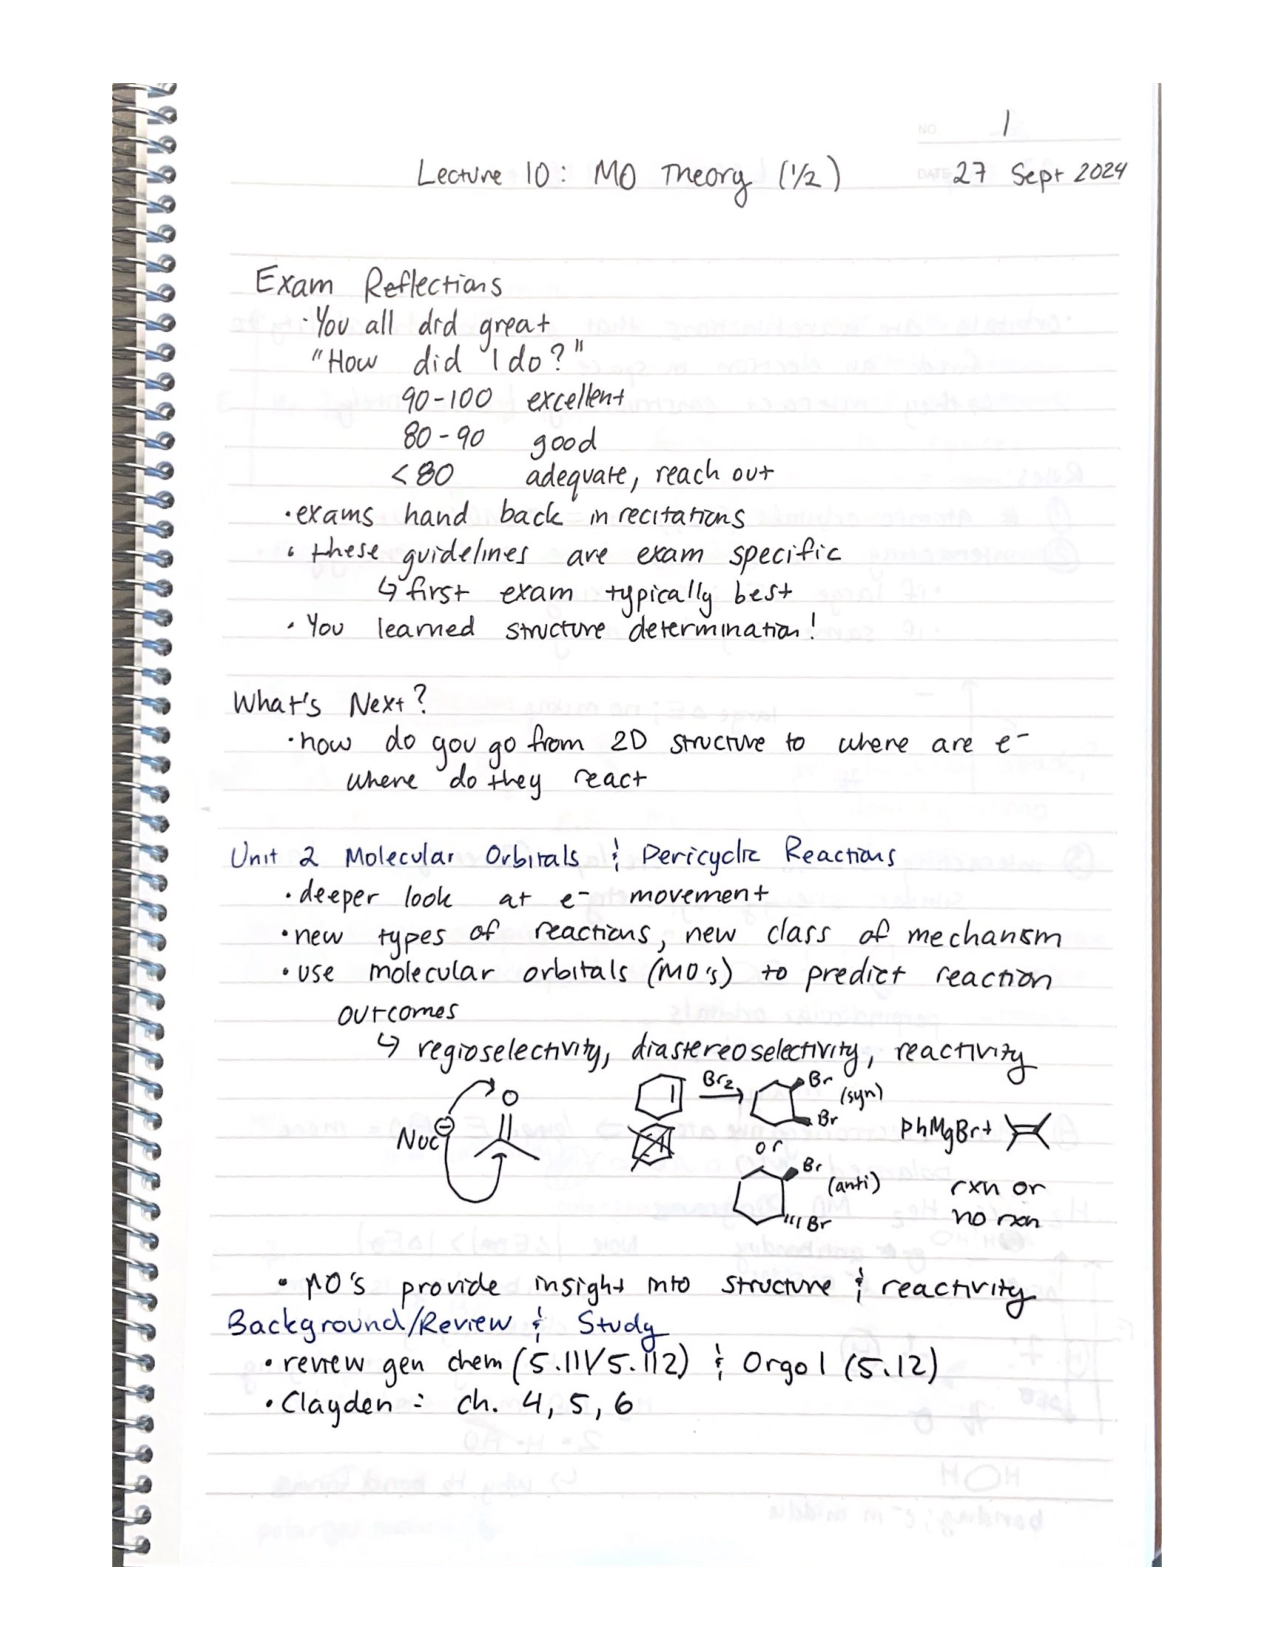
\includepdf[pages=-]{BlackboardPics/L10/L10Notes-Eastham.pdf}



\section{Molecular Orbital Theory - 2}
\begin{itemize}
    \item \marginnote{9/30:}Lecture 10 recap: What MO theory can explain.
    \begin{figure}[h!]
        \centering
        \footnotesize
        \setchemfig{atom sep=1.4em}
        \begin{subfigure}[b]{0.33\linewidth}
            \centering
            \schemestart
                \chemfig{@{N}\charge{30=$\ominus$}{Nuc}}
                \arrow{0}
                \chemfig{-[:30]@{C}(=[2]@{O}O)-[:-30]}
            \schemestop
            \chemmove{
                \draw [curved arrow={11pt}{1pt},gray,densely dashed] (N) to[out=30,in=150] (O);
                \draw [curved arrow={11pt}{2pt}] (N) to[out=30,in=-100,in looseness=1.5] (C);
            }
            \vspace{3.9em}
            \caption{A regioselective reaction.}
            \label{fig:MOexplainsa}
        \end{subfigure}
        \begin{subfigure}[b]{0.32\linewidth}
            \centering
            \setchemfig{autoreset cntcycle=false}
            \schemestart
                \chemfig{*6(--=---)}
                \arrow(c1--c23){0}[,1.5]
                \subscheme{
                    \chemfig{*6(--(<Br)-(<Br)---)}
                    \arrow(c2--c3){0}[-90,0.5]
                    \chemfig{*6(--(<:Br)-(<Br)---)}
                }
            \schemestop
            \chemmove{
                \draw ([xshift=9pt]c1.east) -- node[above]{\ce{Br2}} ($(c1)!0.5!(c23)$) coordinate (c25) -- (c25 |- c2) -- ([xshift=-9pt]c2.west);
                \draw (c25) -- (c25 |- c3) -- ([xshift=-9pt]c3.west);
                \node [magenta] at (cyclecenter2) {X};
                \node [magenta] at (cyclecenter3) {$\checkmark$};
            }
            \caption{A diasterioselective reaction.}
            \label{fig:MOexplainsb}
        \end{subfigure}
        \begin{subfigure}[b]{0.33\linewidth}
            \centering
            \schemestart
                \chemfig{PhMgBr}
                \arrow{0}[,0.1]\+{,,1em}
                \chemfig{-[:60](-[:120])=(-[:60])-[:-60]}
                \arrow(c1--c23){0}
                \subscheme{
                    \chemfig{rxn}
                    \arrow(c2--c3){0}[-90,0.5]
                    \chemfig{{no\ rxn}}
                }
            \schemestop
            \chemmove{
                \draw ([xshift=9pt]c1.east) -- ($(c1)!0.6!(c23)$) coordinate (c25) -- (c25 |- c2) -- ([xshift=-9pt]c2.west);
                \draw (c25) -- (c25 |- c3) -- ([xshift=-9pt]c3.west);
                \node [magenta,above] at (c2.north) {X};
                \node [magenta,below] at (c3.south) {$\checkmark$};
            }
            \vspace{3.65em}
            \caption{An unreactive mixture.}
            \label{fig:MOexplainsc}
        \end{subfigure}\\[2em]
        \setchemfig{atom sep=3em}
        \begin{subfigure}[b]{0.33\linewidth}
            \centering
            \vspace{1em}
            \schemestart
                \chemfig{@{N}\charge{30=$\ominus$}{Nuc}}
                \arrow{0}[-35,0.6]
                \chemfig{@{C}C(<:[:160]R)(<[:-160]R)-@{O}O}
            \schemestop
            \chemmove{
                \filldraw [thick,draw=orx,fill=white,rotate around={ 17:(C)}] ($(C)+(0.0018,0.2)$) to[bend right=120,looseness=900] ($(C)+(-0.0018,0.2)$) -- cycle;
                \filldraw [thick,draw=orx,fill=ory  ,rotate around={-17:(C)}] ($(C)+(0.0018,-0.2)$) to[bend left=120,looseness=900] ($(C)+(-0.0018,-0.2)$) -- cycle;
                \filldraw [thick,draw=orx,fill=ory  ,rotate around={-17:(O)}] ($(O)+(0.0018,0.2)$) to[bend right=120,looseness=500] ($(O)+(-0.0018,0.2)$) -- cycle;
                \filldraw [thick,draw=orx,fill=white,rotate around={ 17:(O)}] ($(O)+(0.0018,-0.2)$) to[bend left=120,looseness=500] ($(O)+(-0.0018,-0.2)$) -- cycle;
                % 
                \draw [curved arrow={11pt}{4em}] (N) to[out=30,in=107,in looseness=3] (C);
            }
            \vspace{1.7em}
            \caption{MO explanation.}
            \label{fig:MOexplainsd}
        \end{subfigure}
        \begin{subfigure}[b]{0.32\linewidth}
            \centering
            \vspace{1.6em}
            \schemestart
                \chemfig{@{N}\charge{30=$\ominus$}{Br}}
                \arrow{0}[50,0.6]
                \chemfig{*3([:-30]@{C1}(-R)-(-R)-@{Br}\charge{[extra sep=5pt]90=$\oplus$}{Br}-[@{3}])}
            \schemestop
            \chemmove{
                \filldraw [thick,draw=orx,fill=ory,rotate around={-30:(C1)}] ($(C1)+(0.0018,0)$) to[bend left=120,looseness=920] ($(C1)+(-0.0018,0)$) -- cycle;
                \draw [thick,draw=orx,rotate around={-30:(C1)}] ($(C1)+(0.0018,0)$) to[bend right=120,looseness=460] ($(C1)+(-0.0018,0)$) -- cycle;
                \filldraw [thick,draw=orx,fill=ory,rotate around={-30:(Br)}] ($(Br)+(0.0018,-0.2)$) to[bend left=120,looseness=300] ($(Br)+(-0.0018,-0.2)$) -- cycle;
                \draw [thick,draw=orx,rotate around={-30:(Br)}] ($(Br)+(0.0018,0.2)$) to[bend right=120,looseness=600] ($(Br)+(-0.0018,0.2)$) -- cycle;
                % 
                \draw [curved arrow={8pt}{3.5em}] (N) to[out=30,in=-110,in looseness=2] (C1);
                \draw [curved arrow={4pt}{1pt}] (3) to[bend left=70,looseness=2.2] (Br);
            }
            \caption{MO explanation.}
            \label{fig:MOexplainse}
        \end{subfigure}
        \begin{subfigure}[b]{0.33\linewidth}
            \centering
            \begin{tikzpicture}
                \draw (-0.5,2) -- ++(-0.5,0) node[left,align=right]{$\pi^*$\\LUMO};
                \draw (0.5,0) -- node{\Large$\upharpoonleft$\hspace{-1mm}$\downharpoonright$} ++(0.5,0) node[right,align=left]{\ce{Ph-}\\HOMO};
                \draw [<->] (0,0) -- node[right]{$\Delta E$} (0,2);
            \end{tikzpicture}
            \caption{MO explanation.}
            \label{fig:MOexplainsf}
        \end{subfigure}
        % \begin{tikzpicture}[remember picture,overlay]
        %     \draw (-15,3.4) -- ++(15,0);
        % \end{tikzpicture}
        \caption{MO theory explains these phenomena.}
        \label{fig:MOexplains}
    \end{figure}
    \begin{itemize}
        \item Regioselectivity.
        \begin{itemize}
            \item Consider a nucleophile adding into a carbonyl (Figure \ref{fig:MOexplainsa}).
            \begin{itemize}
                \item Experimentally, we observe that the nucleophile attacks the carbon atom (magenta arrow) instead of the oxygen atom (grey dashed arrow).
            \end{itemize}
            \item To understand why, we must consider the carbonyl's molecular orbitals (Figure \ref{fig:MOexplainsd}).
            \begin{itemize}
                \item Specifically, we must consider the carbonyl's LUMO, since this will be the MO that interacts with the nucleophile's HOMO. Here, the LUMO is the carbonyl's $\pi^*$-orbital.
                \item The carbonyl's LUMO has big lobes on carbon and small lobes on oxygen; in other words, this LUMO is \textbf{polarized} toward carbon.
                \item The difference in lobe size explains why the nucleophile attacks carbon instead of oxygen.
            \end{itemize}
        \end{itemize}
        \item Diastereoselectivity.
        \begin{itemize}
            \item Consider the bromination of an alkene (Figure \ref{fig:MOexplainsb}).
            \begin{itemize}
                \item Experimentally, we observe that the \emph{anti} adduct is formed instead of the \emph{syn} adduct.
            \end{itemize}
            \item To understand why, we consider the MOs of the bromonium ion intermediate (Figure \ref{fig:MOexplainse}).
            \begin{itemize}
                \item For the same reason as before, we must consider the bromonium ion's LUMO. Here, the LUMO is the \ce{C-Br} $\sigma^*$-orbital.
                \item The bromonium ion's LUMO has its largest lobe behind carbon.
                \item Thus, this is the lobe that will be attacked by the \ce{Br-} nucleophile. Such an attack is called a "backside attack" and induces the \emph{anti} product.
            \end{itemize}
        \end{itemize}
        \item Reactivity.
        \begin{itemize}
            \item Consider a Grignard reagent adding into an olefin (Figure \ref{fig:MOexplainsc}).
            \begin{itemize}
                \item Experimentally, we observe no reaction here.
            \end{itemize}
            \item To understand why, we must consider the relative energies of the reacting MOs (Figure \ref{fig:MOexplainsf}).
            \begin{itemize}
                \item Essentially, the alkene's LUMO (a $\pi^*$-orbital) is much higher in energy than the phenyl anion's HOMO. Thus, the $\Delta E$ gap is too big, i.e., there is a lack of energy symmetry.
                \item Therefore, by Rule 3 from Lecture 10, no reaction occurs.
            \end{itemize}
        \end{itemize}
    \end{itemize}
    \pagebreak
    \item Today: More MO theory.
    \item Lecture outline.
    \begin{itemize}
        \item The B\"{u}rgi-Dunitz angle.
        \item Hyperconjugation.
        \item The anomeric effect.
        \item Stereoelectronic effects and the rate of reaction.
    \end{itemize}
    \item \textbf{B\"{u}rgi-Dunitz angle}: The angle at which nucleophiles typically add to carbonyls. \emph{Given by} \ang{107}.
    \begin{figure}[h!]
        \centering
        \footnotesize
        \setchemfig{atom sep=3em}
        \begin{subfigure}[b]{0.3\linewidth}
            \centering
            \schemestart
                \chemfig{@{C}C(<:[:160]R)(<[:-160]R)(-[:107,,,,<-]@{N}Nuc)=@{O}O}
            \schemestop
            \chemmove{
                \pic [draw,-,shorten <=4pt,shorten >=2pt,angle eccentricity=1.6,angle radius=6mm,pic text={\ang{107}}] {angle=O--C--N};
            }
            \vspace{2.5em}
            \caption{Definition.}
            \label{fig:BDanglea}
        \end{subfigure}
        \begin{subfigure}[b]{0.3\linewidth}
            \centering
            \vspace{1em}
            \schemestart
                \chemfig{@{N}\charge{[extra sep=2.2em]-73=$\ominus$}{Nuc}}
                \arrow{0}[-72,1.2]
                \chemfig{@{C}C(<:[:160]R)(<[:-160]R)-[@{1}]@{O}O}
            \schemestop
            \chemmove{
                \filldraw [thick,draw=orx,fill=white,rotate around={ 17:(C)}] ($(C)+(0.0018,0.2)$) to[bend right=120,looseness=900] ($(C)+(-0.0018,0.2)$) -- cycle;
                \filldraw [thick,draw=orx,fill=ory  ,rotate around={-17:(C)}] ($(C)+(0.0018,-0.2)$) to[bend left=120,looseness=900] ($(C)+(-0.0018,-0.2)$) -- cycle;
                \filldraw [thick,draw=orx,fill=ory  ,rotate around={-17:(O)}] ($(O)+(0.0018,0.2)$) to[bend right=120,looseness=500] ($(O)+(-0.0018,0.2)$) -- cycle;
                \filldraw [thick,draw=orx,fill=white,rotate around={ 17:(O)}] ($(O)+(0.0018,-0.2)$) to[bend left=120,looseness=500] ($(O)+(-0.0018,-0.2)$) -- cycle;
                % 
                \draw [thick,draw=orx,rotate around={17:(N)}] ($(N)+(0.0018,-0.2)$) to[bend left=120,looseness=900] ($(N)+(-0.0018,-0.2)$) -- cycle;
                % 
                \draw (C) ++(107:1.3) -- node[right]{\scriptsize Yes!} ++(107:-0.2);
                \draw (C) ++(-107:1.3) -- node[right]{\scriptsize Yes!} ++(-107:-0.2);
                \draw (C) ++(180:1.3) node[left,align=center]{\scriptsize No!\\(*)} -- ++(180:-0.2);
                % 
                \draw (O) ++(73:0.94) -- node[right]{\scriptsize No!} ++(73:-0.2);
                \draw (O) ++(-73:0.94) -- node[right]{\scriptsize No!} ++(-73:-0.2);
                % 
                \draw (1) ++(-90:0.4) node[below]{\scriptsize No!} -- ++(-90:-0.2);
            }
            \vspace{2.5em}
            \caption{Effective overlap.}
            \label{fig:BDangleb}
        \end{subfigure}
        \caption{B\"{u}rgi-Dunitz angle.}
        \label{fig:BDangle}
    \end{figure}
    \begin{itemize}
        \item This is the angle between the new \ce{C-Nuc} bond and the carbonyl's $\sigma$-plane (Figure \ref{fig:BDanglea}).
        \item Nucleophiles attack at this angle because it's the location of the $\pi^*$-lobe on carbon (Figure \ref{fig:MOexplainsd}).
        \item Let's elaborate a bit on Figure \ref{fig:MOexplainsd} now (Figure \ref{fig:BDangleb}).
        \begin{itemize}
            \item Once again, consider the carbonyl $\pi^*$-orbital (its LUMO) and its "butterfly" lobes.
            \item The nucleophile must approach the $\pi^*$-orbital with the right symmetry. This is why we see its HOMO's lobe approach the carbon atom's $\pi^*$-lobe dead-on at exactly the right angle.
            \begin{itemize}
                \item This angle leads to efficient overlap, and hence an effective sharing of electron density.
                \item This is an example of Rule 3 from Lecture 10.
            \end{itemize}
            \item Are there any other locations at which we can add into the carbonyl?
            \begin{itemize}
                \item We can also add into the shaded carbon $\pi^*$-lobe on the other side of the $\sigma$-plane by reversing the shading of the nucleophile's lobe!
                \item However, any other angle of attack will \emph{not} work.
                \item Note (*): A backside attack is good for interacting with the $\sigma^*$-orbital, but bad for interacting with the $\pi^*$-orbital that we need for carbonyl chemistry.
            \end{itemize}
        \end{itemize}
    \end{itemize}
    \item \textbf{Hyperconjugation}: The mixing of filled and empty orbitals to stabilize a system.
    \item Example (from 5.12): Stabilizing carbocations.
    \begin{figure}[H]
        \centering
        \footnotesize
        \setchemfig{atom sep=3em}
        \begin{subfigure}[b]{0.3\linewidth}
            \centering
            \chemfig{@{C1}\charge{[extra sep=2em]90=$\oplus$}{C}(<:[:160]R)(<[:-160]R)-@{C2}C(<:[:20]H)(<[:-20]H)-[@{1}2]@{H}H}
            \chemmove{
                \draw [thick,orx] ($(C1)+(0.0018,0.2)$) to[bend right=120,looseness=900] ($(C1)+(-0.0018,0.2)$) -- cycle;
                \filldraw [thick,draw=orx,fill=ory] ($(C1)+(0.0018,-0.2)$) to[bend left=120,looseness=900] ($(C1)+(-0.0018,-0.2)$) -- cycle;
                % 
                \draw [thick,orx] (H) circle (2mm);
                \draw [thick,orx] (1) ellipse (1.7mm and 3.4mm);
                \filldraw [thick,draw=orx,fill=ory] ($(C2)+(0.0018,-0.2)$) to[bend left=130,looseness=500] ($(C2)+(-0.0018,-0.2)$) -- cycle;
                % 
                \draw [curved arrow={7pt}{8pt}] ([yshift=6mm]C2.center) to[bend right=35,looseness=1.3] ([yshift=6mm]C1.center);
            }
            \vspace{3.74em}
            \caption{$1^\circ$ carbocation.}
            \label{fig:hyperconjugationCCa}
        \end{subfigure}
        \begin{subfigure}[b]{0.3\linewidth}
            \centering
            \chemfig{@{C1}\charge{[extra sep=2em]90=$\oplus$}{C}(<:[:155,1.4]R_2@{C2}C-[@{2}2,,2]@{H2}H)(<[:-130,1.2]R_2@{C3}C-[@{3}2,,2]@{H3}H)-[,1.2]@{C4}CR_2-[@{4}2]@{H4}H}
            \chemmove{
                \draw [thick,orx] ($(C1)+(0.0018,0.2)$) to[bend right=120,looseness=900] ($(C1)+(-0.0018,0.2)$) -- cycle;
                \filldraw [thick,draw=orx,fill=ory] ($(C1)+(0.0018,-0.2)$) to[bend left=120,looseness=900] ($(C1)+(-0.0018,-0.2)$) -- cycle;
                % 
                \draw [thick,orx] (H2) circle (2mm);
                \draw [thick,orx] (2) ellipse (1.7mm and 3.4mm);
                \filldraw [thick,draw=orx,fill=ory] ($(C2)+(0.0018,-0.2)$) to[bend left=130,looseness=500] ($(C2)+(-0.0018,-0.2)$) -- cycle;
                % 
                \draw [thick,orx] (H3) circle (2mm);
                \draw [thick,orx] (3) ellipse (1.7mm and 3.4mm);
                \filldraw [thick,draw=orx,fill=ory] ($(C3)+(0.0018,-0.2)$) to[bend left=130,looseness=500] ($(C3)+(-0.0018,-0.2)$) -- cycle;
                % 
                \draw [thick,orx] (H4) circle (2mm);
                \draw [thick,orx] (4) ellipse (1.7mm and 3.4mm);
                \filldraw [thick,draw=orx,fill=ory] ($(C4)+(0.0018,-0.2)$) to[bend left=130,looseness=500] ($(C4)+(-0.0018,-0.2)$) -- cycle;
                % 
                \draw [curved arrow={7pt}{8pt}] ([yshift=6mm]C4.center) to[bend right=35,looseness=1.3] ([yshift=6mm]C1.center);
                \draw [curved arrow={7pt}{10pt}] ([yshift=6mm]C2.center) to[bend left=30,looseness=1.2] ([yshift=6mm]C1.center);
                \draw [curved arrow={7pt}{6pt}] ([yshift=6mm]C3.center) to[bend right=20,looseness=1.1] ([xshift=-1mm,yshift=6mm]C1.center);
            }
            \vspace{1.5em}
            \caption{$3^\circ$ carbocation.}
            \label{fig:hyperconjugationCCb}
        \end{subfigure}
        % \begin{tikzpicture}[remember picture,overlay]
        %     \draw (-10,2.2) -- ++(15,0);
        % \end{tikzpicture}
        \caption{Hyperconjugation stabilizes carbocations.}
        \label{fig:hyperconjugationCC}
    \end{figure}
    \begin{itemize}
        \item Consider a primary ($1^\circ$) carbocation (Figure \ref{fig:hyperconjugationCCa}).
        \begin{itemize}
            \item In a carbocation, the positively charged carbon localizes its lack of electron density to an empty $p$-orbital.
            \item However, adjacent to this empty $p$-orbital is a full $\sigma$-orbital, namely, the adjacent \ce{C-H} bond. Moreover, this bond has the right \emph{geometry} to donate into the empty $p$-orbital.
            \item Thus, the $\sigma$-orbital of the \ce{C-H} bond will donate electron density into the empty $p$-orbital, delocalizing both positive and negative charges and thereby stabilizing the system.
        \end{itemize}
        \item We denote hyperconjugation interactions using a special \textbf{notation}; the particular hyperconjugation in Figure \ref{fig:hyperconjugationCC} is denoted $\sigma_{\ce{CH}}\to p_{\ce{C}}$.\footnote{This is pronounced "sigma \ce{C-H} to $p$ C donation" or (very explicitly) "sigma see aech to pee see donation."}
        \item In a tertiary ($3^\circ$) carbocation, we get electron donation from \emph{three} adjacent $\sigma_{\ce{CH}}$ orbitals.
        \begin{itemize}
            \item These \emph{three} stabilizing interactions explain why $3^\circ$ carbocations are more stable than $1^\circ$ ones!
            \item Such effects are also why more substituted cations are more stable in general.
        \end{itemize}
    \end{itemize}
    \item \textbf{Hyperconjugation notation}: The concise method for denoting a certain hyperconjugative orbital interaction. \emph{Given by}
    \begin{equation*}
        \text{orbital\textsubscript{atoms}} \to \text{orbital\textsubscript{atoms}}
    \end{equation*}
    \begin{itemize}
        \item The arrow means "donates into."
        \begin{itemize}
            \item Indeed, we always write the filled orbital first (before the arrow) and the empty orbital second (after the arrow).
        \end{itemize}
        \item Possible orbitals: $\sigma,\sigma^*,\pi,\pi^*,p,n$.
        \begin{itemize}
            \item Note that $n$ denotes a \underline{n}onbonding lone pair.
        \end{itemize}
    \end{itemize}
    \item \textbf{Anomeric effect}: The tendency of heteroatom substituents adjacent to heteroatoms in cyclohexane derivatives to prefer the axial orientation.
    \item Let's break this rather complicated definition down through an example.
    \begin{figure}[H]
        \centering
        \footnotesize
        \setchemfig{fixed length=false}
        \begin{subfigure}[b]{0.49\linewidth}
            \centering
            \schemestart
                \chemfig{?-[:20](-[2,,,,white]\phantom{H})-[:-50](-[:20]OMe)-[:170]-[:-160]-[:130]?}
                \arrow(.-13--.-167){<<->}
                \chemfig{?(-[2]@{H1}H)-[:-20]-[:10](-[2]@{O}OMe)-[:-130]-[:160](-[2,,,,ovbnd]@{H2}H)-[:-170]?}
            \schemestop
            \chemmove{
                \draw [-,cyan,thick] ([xshift=2pt,yshift=2pt]H1.50) to[out=-40,in=40] ([xshift=2pt,yshift=-2pt]H1.-50);
                \draw [-,cyan,thick] ([xshift=2pt,yshift=2pt]H2.50) to[out=-40,in=40] ([xshift=2pt,yshift=-2pt]H2.-50);
                \draw [-,cyan,thick] ([xshift=-2pt,yshift=2pt]O.130) to[out=-140,in=140] ([xshift=-2pt,yshift=-2pt]O.-130);
            }
            \caption{Sterics win in methoxycyclohexane.}
            \label{fig:anomerica}
        \end{subfigure}
        \begin{subfigure}[b]{0.49\linewidth}
            \centering
            \schemestart
                \chemfig{?-[:20]-[:-50](-[:20]OMe)-[:170]O-[:-160]-[:130]?(-[2,,,,white]\phantom{OMe})}
                \arrow(.-10--.-170){<->>}
                \chemfig{?-[:-20]-[:10](-[2]OMe)-[:-130]O-[:160]-[:-170]?}
            \schemestop
            \caption{Anomeric wins in 2-methoxytetrahydropyran.}
            \label{fig:anomericb}
        \end{subfigure}\\[2em]
        \begin{subfigure}[b]{\linewidth}
            \centering
            \setchemfig{atom sep=3em}
            \schemestart
                \chemfig{?-[:20]-[:-50]@{C2}(-[:20]@{O2}O-[:-40])-[:170]@{O1}\charge{[extra sep=2.6em]90=\:}{\charge{[extra sep=2em]-50=\:}{O}}-[:-160]-[:130]?(-[2,,,,white]\phantom{O}-[:60,,,,white])}
                \arrow(.-10--.-170){<->>}[,2]
                \chemfig{?-[:-20]-[:10]@{C2b}(-[2]@{O2b}O-[:30])-[:-130]@{O1b}\charge{[extra sep=2.6em]-90=\:}{\charge{[extra sep=2.4em]20=\:}{O}}-[:160]-[:-170]?}
            \schemestop
            \chemmove{
                \draw [thick,orx,rotate around={-70:(C2)}] ($(C2)+(0.0018,0)$) to[bend left=120,looseness=920] ($(C2)+(-0.0018,0)$) -- cycle;
                \filldraw [thick,draw=orx,fill=ory,rotate around={-70:(C2)}] ($(C2)+(0.0018,0)$) to[bend right=120,looseness=460] ($(C2)+(-0.0018,0)$) -- cycle;
                \draw [thick,orx,rotate around={-70:(O2)}] ($(O2)+(0.0018,-0.2)$) to[bend left=120,looseness=300] ($(O2)+(-0.0018,-0.2)$) -- cycle;
                \filldraw [thick,draw=orx,fill=ory,rotate around={-70:(O2)}] ($(O2)+(0.0018,0.2)$) to[bend right=120,looseness=600] ($(O2)+(-0.0018,0.2)$) -- cycle;
                % 
                \draw [line width=3pt,white] ($(O1)+(0.0018,0.2)$) to[bend right=120,looseness=900] ($(O1)+(-0.0018,0.2)$) -- cycle;
                \draw [line width=3pt,white,rotate around={-140:(O1)}] ($(O1)+(0.0018,0.2)$) to[bend right=120,looseness=900] ($(O1)+(-0.0018,0.2)$) -- cycle;
                \fill [white] ($(O1)+(0.0018,0.2)$) to[bend right=120,looseness=400] ($(O1)+(-0.0018,0.2)$) -- cycle;
                \fill [white,rotate around={-140:(O1)}] ($(O1)+(0.0018,0.2)$) to[bend right=125,looseness=750] ($(O1)+(-0.0018,0.2)$) -- cycle;
                \draw [thick,orx] ($(O1)+(0.0018,0.2)$) to[bend right=120,looseness=900] ($(O1)+(-0.0018,0.2)$) -- cycle;
                \draw [thick,orx,rotate around={-140:(O1)}] ($(O1)+(0.0018,0.2)$) to[bend right=120,looseness=900] ($(O1)+(-0.0018,0.2)$) -- cycle;
                % 
                \draw [curved arrow={3.1em}{2.2em},gray,densely dashed] (O1) to[out=-45,in=10,looseness=3.5] (O2);
            }
            \chemmove{
                \draw [thick,orx] ($(C2b)+(0.0018,0)$) to[bend left=120,looseness=920] ($(C2b)+(-0.0018,0)$) -- cycle;
                \filldraw [thick,draw=orx,fill=ory] ($(C2b)+(0.0018,0)$) to[bend right=120,looseness=460] ($(C2b)+(-0.0018,0)$) -- cycle;
                \draw [thick,orx] ($(O2b)+(0.0018,-0.2)$) to[bend left=120,looseness=300] ($(O2b)+(-0.0018,-0.2)$) -- cycle;
                \filldraw [thick,draw=orx,fill=ory] ($(O2b)+(0.0018,0.2)$) to[bend right=120,looseness=600] ($(O2b)+(-0.0018,0.2)$) -- cycle;
                % 
                \draw [line width=3pt,white,rotate around={-70:(O1b)}] ($(O1b)+(0.0018,0.2)$) to[bend right=120,looseness=900] ($(O1b)+(-0.0018,0.2)$) -- cycle;
                \fill [white,rotate around={-70:(O1b)}] ($(O1b)+(0.0018,0.2)$) to[bend right=127,looseness=794] ($(O1b)+(-0.0018,0.2)$) -- cycle;
                \draw [thick,orx,rotate around={-70:(O1b)}] ($(O1b)+(0.0018,0.2)$) to[bend right=120,looseness=900] ($(O1b)+(-0.0018,0.2)$) -- cycle;
                \draw [thick,orx] ($(O1b)+(0.0018,-0.2)$) to[bend left=120,looseness=900] ($(O1b)+(-0.0018,-0.2)$) -- cycle;
                % 
                \draw [curved arrow={3.3em}{3.3em}] (O1b) to[out=-90,in=-90,looseness=4.5] (C2b);
            }
            \vspace{4em}
            \caption{MOs explain the anomeric effect.}
            \label{fig:anomericc}
        \end{subfigure}\\[2em]
        \begin{subfigure}[b]{0.37\linewidth}
            \centering
            \schemestart
                \chemfig{?-[:-20]-[:10](-[@{2}2]@{O2}OMe)-[@{1}:-130]@{O1}O-[:160]-[:-170]?}
                \arrow{<->}
                \chemfig{?-[:-20]-[:10](-[2,,,,white]\charge{135=$\ominus$}{O}Me)=^[:-130]\charge{-45=$\oplus$}{O}-[:160]-[:-170]?}
            \schemestop
            \chemmove{
                \draw [curved arrow={1pt}{2pt}] (O1) to[bend right=70,looseness=2.5] (1);
                \draw [curved arrow={2pt}{1pt}] (2) to[bend left=70,looseness=2.5] (O2);
            }
            \vspace{0.7em}
            \caption{Resonance explains the anomeric effect.}
            \label{fig:anomericd}
        \end{subfigure}
        \caption{Anomeric effect.}
        \label{fig:anomeric}
    \end{figure}
    \begin{itemize}
        \item In methoxycyclohexane, the methoxy group prefers to be equatorial to avoid 1,3-diaxial interactions (Figure \ref{fig:anomerica}).
        \begin{itemize}
            \item This leads to a $70:30$ distribution in favor of the equatorial conformer.
        \end{itemize}
        \item However, in 2-methoxytetrahydropyran, the methoxy group prefers to be \emph{axial} due to the anomeric effect (Figure \ref{fig:anomericb}).
        \begin{itemize}
            \item This \emph{also} leads to a $70:30$ distribution, but this time in favor of the axial conformer.
            \item Notice how this empirical observation reflects the definition of the anomeric effect: We have a heteroatom substituent (the methoxy group) adjacent to a heteroatom in cyclohexane (the oxygen in the six-membered ring), and it is prefering the axial orientation!
        \end{itemize}
        \item What causes the anomeric effect? Let's investigate the stabilization of the axial conformer further using molecular orbitals (Figure \ref{fig:anomericc}).
        \begin{itemize}
            \item In 2-methoxytetrahydropyran's equatorial conformation, we get poor overlap between the oxygen lone pair's orbital and the \ce{C-OMe} antibonding orbital. This poor overlap is due to the \emph{gauche} orientation of said orbitals.
            \item In 2-methoxytetrahydropyran's axial conformation, we get really nice overlap between the oxygen lone pair and the $\sigma^*$-orbital of the \ce{C-OMe} bond. This is because both orbitals have large lobes pointing axial down. Because of this favorable geometry, $n_{\ce{O}}\to\sigma_{\ce{CO}}^*$ hyperconjugation occurs.\footnote{Note that there is no particular reason why overlap with a $\sigma^*$-orbital, in particular, is stabilizing. Rather, the point is that we have a filled orbital (the lone pair) adjacent to an empty orbital (which just happens to be a $\sigma^*$ orbital), so hyperconjugation can occur to spread out the negative and positive charges. This delocalization --- like any --- is then inherently stabilizing.}
        \end{itemize}
        \item Another way of showing how the anomeric effect stabilizes the axial conformer is by using resonance diagrams (Figure \ref{fig:anomericd}).
        \begin{itemize}
            \item Indeed, starting from the typical picture, we can push the lone pair into an \ce{O=C} $\pi$-bond and formally break the \ce{C-OMe} $\sigma$-bond.
            \item The result is called a \textbf{no-bond resonance form}.
            \item Something should feel off to you here, though.
            \begin{itemize}
                \item When you learned to draw resonance structures, you learned that you can't break $\sigma$-bonds.
                \item However, we are now telling you that sometimes, you \emph{are} allowed to break $\sigma$-bonds. This is "next-level resonance structures."
            \end{itemize}
            \item Note that 2-methoxytetrahydropyran doesn't go all the way to the no-bond resonance form, but said resonance form \emph{is} a major contributor.
            \begin{itemize}
                \item This also means that the no-bond resonance form affects the reactivity of the molecule.
            \end{itemize}
        \end{itemize}
    \end{itemize}
    \item Both hyperconjugation and the anomeric effect fall under the broader category of \textbf{stereoelectronic effects}.
    \begin{itemize}
        \item Note that they are not the only examples of such effects, though.
    \end{itemize}
    \item \textbf{Stereoelectronic effect}: An effect on structure or reactivity of a molecule caused by the spatial orientation of its orbitals.
    \begin{itemize}
        \item We've previously learned that everything in Orgo can be explained by steric and electronic effects, but stereoelectronic effects are like a secret third option!
    \end{itemize}
    \item Let's now look at some more places where stereoelectronic effects crop up.
    \pagebreak
    \item Example: Hyperconjugation in noncationic species.
    \begin{figure}[H]
        \centering
        \footnotesize
        \begin{subfigure}[b]{0.4\linewidth}
            \centering
            \schemestart
                \chemname{\chemfig{H-[:-60](<:[:-150]H)(<[:-120]H)-(<:[:60]H)(<[:30]H)-[:-60]H}}{Staggered}
                \arrow{<<->}
                \chemname{\chemfig{H-[:-60](<:[:-150]H)(<[:-120]H)-(<[:-60]H)(<:[:-30]H)-[:60]H}}{Eclipsed}
            \schemestop
            \caption{Ethane's conformers.}
            \label{fig:ethaneStaggereda}
        \end{subfigure}
        \begin{subfigure}[b]{0.4\linewidth}
            \centering
            \chemfig[atom sep=3em]{@{H1}H-[@{1}:-60]@{C1}C-@{C2}C-[:-60]@{H2}H}
            \chemmove{
                \draw [thick,orx] (H1) circle (2mm);
                \draw [thick,orx,rotate around={30:(1)}] (1) ellipse (1.7mm and 3.4mm);
                \filldraw [thick,draw=orx,fill=ory,rotate around={30:(C1)}] ($(C1)+(0.0018,-0.2)$) to[bend left=130,looseness=500] ($(C1)+(-0.0018,-0.2)$) -- cycle;
                % 
                \draw [thick,orx] (H2) circle (2mm);
                \filldraw [thick,draw=orx,fill=ory,rotate around={30:(C2)}] ($(C2)+(0.0018,-0.2)$) to[bend left=120,looseness=730] ($(C2)+(-0.0018,-0.2)$) -- cycle;
                \draw [thick,orx,rotate around={30:(C2)}] ($(C2)+(0.0018,0.2)$) to[bend right=130,looseness=500] ($(C2)+(-0.0018,0.2)$) -- cycle;
                % 
                \draw [curved arrow={0pt}{1.6em}] ([xshift=-1pt,yshift=5mm]C1.north) to[bend left=30] ([yshift=2mm]C2.north);
            }
            \caption{$\sigma_{\ce{CH}}\to\sigma_{\ce{CH}}^*$ stabilization.}
            \label{fig:ethaneStaggeredb}
        \end{subfigure}
        \caption{Hyperconjugation stabilizes staggered ethane.}
        \label{fig:ethaneStaggered}
    \end{figure}
    \begin{itemize}
        \item We may have learned that ethane prefers the staggered conformer over the eclipsed conformer (Figure \ref{fig:ethaneStaggereda}) due to sterics.
        \begin{itemize}
            \item This is not true!
            \item We know this because \ce{H} is really tiny.
        \end{itemize}
        \item In fact, this preference is due to hyperconjugation, a stereoelectronic effect (Figure \ref{fig:ethaneStaggeredb}).
        \begin{itemize}
            \item Staggered ethane is stabilized by electron donation from the $\sigma$-bond of one \ce{C-H} bond into the adjacent, antiperiplanar \ce{C-H} bond's $\sigma^*$ orbital: $\sigma_{\ce{CH}}\to\sigma_{\ce{CH}}^*$.
            \item This is a small interaction, but it occurs six times, once for each \ce{C-H} $\sigma$-bond!
        \end{itemize}
        \item Takeaway: Electron delocalization is stabilizing, and more delocalization is more stabilizing.
    \end{itemize}
    \item Example: Stereoelectronic stabilization can accelerate reactions.
    \begin{figure}[H]
        \centering
        \footnotesize
        \chemnameinit{}
        \begin{subfigure}[b]{0.45\linewidth}
            \centering
            \schemestart
                \chemfig{*6(---(-Br)---)}
                \arrow{->[\ce{MeOH}]}[,1.2]
                \chemfig{*6(---(-OMe)---)}
            \schemestop
            \caption{S\textsubscript{N}1 without an adjacent heteroatom.}
            \label{fig:stereoelectronicRxna}
        \end{subfigure}
        \begin{subfigure}[b]{0.45\linewidth}
            \centering
            \schemestart
                \chemfig{*6(---(-Br)-O--)}
                \arrow{->[\ce{MeOH}]}[,1.2]
                \chemfig{*6(---(-OMe)-O--)}
            \schemestop
            \caption{S\textsubscript{N}1 with an adjacent heteroatom.}
            \label{fig:stereoelectronicRxnb}
        \end{subfigure}\\[2em]
        \begin{subfigure}[b]{\linewidth}
            \centering
            \schemestart
                \chemfig{*6(---(-[@{a1}]@{aBr}Br)---)}
                \arrow{->[][-\ce{Br-}]}[,1.2]
                \chemfig{*6(---@{bC}\charge{[extra sep=5pt]30=$\oplus$}{}---)}
                \arrow(--.-170){->[\chemfig{Me@{cO}\charge{90=\:}{O}H}]}[,1.2]
                \chemname{
                    \chemfig{*6(---(-@{dO}\charge{[extra sep=5pt]-90=$\oplus$}{O}(-[@{d1}2]@{dH}H)-[:-30])---)}
                }{Oxonium}
                \arrow(.-10--){->[\chemfig{@{eBr}\charge{45=$\ominus$}{Br}}]}[,1.2]
                \chemfig{*6(---(-OMe)---)}
            \schemestop
            \chemmove{
                \draw [curved arrow={2pt}{2pt}] (a1) to[bend left=70,looseness=2] (aBr);
                \draw [curved arrow={5pt}{10pt}] (cO) to[out=90,in=30,looseness=1.7] (bC);
                \draw [curved arrow={9pt}{1pt}] (eBr) to[out=45,in=0,looseness=1.7] (dH);
                \draw [curved arrow={2pt}{2pt}] (d1) to[bend right=70,looseness=2] (dO);
            }
            \caption{No heteroatom mechanism.}
            \label{fig:stereoelectronicRxnc}
        \end{subfigure}\\[2em]
        \begin{subfigure}[b]{\linewidth}
            \centering
            \schemestart
                \chemfig{*6(---(-[@{a1}]@{aBr}Br)-O--)}
                \arrow{->[][-\ce{Br-}]}[,1.2]
                \chemleft{[}
                    \subscheme{
                        \chemfig{*6(---\charge{[extra sep=5pt]30=$\oplus$}{}-[@{b1}]@{bO}\charge{90=\:}{O}--)}
                        \arrow{<->}
                        \chemfig{*6(-@{cC}--=\charge{[extra sep=5pt]90=$\oplus$}{O}--)}
                    }
                \chemright{]}
                \arrow[,1.2]
                \chemfig{...}
            \schemestop
            \chemmove{
                \draw [curved arrow={2pt}{2pt}] (a1) to[bend left=70,looseness=2] (aBr);
                \draw [curved arrow={5pt}{2pt}] (bO) to[out=90,in=60,looseness=3] (b1);
                \node [below=1mm] at (cC) {Oxocarbenium};
            }
            \vspace{1.2em}
            \caption{Possible heteroatom-promoted mechanism.}
            \label{fig:stereoelectronicRxnd}
        \end{subfigure}\\[2em]
        \begin{subfigure}[b]{\linewidth}
            \centering
            \schemestart
                \chemfig{*6(---(-[@{a2}]@{aBr}Br)-[@{a1}]@{aO}\charge{90=\:}{O}--)}
                \arrow{->[][-\ce{Br-}]}[,1.2]
                \chemfig{*6(---@{bC}=\charge{[extra sep=5pt]90=$\oplus$}{O}--)}
                \arrow(--.-160){->[\chemfig{Me@{cO}\charge{90=\:}{O}H}]}[,1.2]
                \chemfig{*6(---(-@{dO}\charge{[extra sep=5pt]-90=$\oplus$}{O}(-[@{d1}2]@{dH}H)-[:-30])-O--)}
                \arrow(.-20--){->[\chemfig{@{eBr}\charge{45=$\ominus$}{Br}}]}[,1.2]
                \chemfig{*6(---(-OMe)-O--)}
            \schemestop
            \chemmove{
                \draw [curved arrow={5pt}{2pt}] (aO) to[out=90,in=60,looseness=3] (a1);
                \draw [curved arrow={2pt}{2pt}] (a2) to[bend right=70,looseness=2] (aBr);
                \draw [curved arrow={5pt}{2pt}] (cO) to[out=90,in=30,looseness=1.7] (bC);
                \draw [curved arrow={9pt}{1pt}] (eBr) to[out=45,in=0,looseness=1.7] (dH);
                \draw [curved arrow={2pt}{2pt}] (d1) to[bend right=70,looseness=2] (dO);
            }
            \caption{Better heteroatom-promoted mechanism.}
            \label{fig:stereoelectronicRxne}
        \end{subfigure}
        \caption{Stereoelectronic effects accelerate reactions.}
        \label{fig:stereoelectronicRxn}
    \end{figure}
    \begin{itemize}
        \item Consider the S\textsubscript{N}1 substitution of bromocyclohexane to methoxycyclohexane (Figure \ref{fig:stereoelectronicRxna}), vs. the S\textsubscript{N}1 substitution of 2-bromotetrahydropyran to 2-methoxytetrahydropyran (Figure \ref{fig:stereoelectronicRxnb}).
        \item Which of these substitutions occurs faster?
        \item To answer this question, let's look at the mechanism of each (Figures \ref{fig:stereoelectronicRxnc}-\ref{fig:stereoelectronicRxnd}).
        \begin{itemize}
            \item Note that in Figure \ref{fig:stereoelectronicRxnc}, either bromide or another equivalent of methanol can do the final deprotonation of the \textbf{oxonium} ion.\footnote{Note that --- comparing the $\pKa$ of protonated methanol to \ce{HBr} --- methanol is actually almost a million times more basic than bromide. As such, for every one time bromide does the final deprotonation, methanol will do it to almost a million other oxonium intermediates. However, it can still be useful to think of bromide as \emph{formally} doing the final deprotonation so as to balance the reaction \ce{C6H11Br + CH3OH -> C6H11OCH3 + HBr}.}
            \item Note that in Figure \ref{fig:stereoelectronicRxnd}, the fact that the \textbf{oxocarbenium} ion obeys the octet rule implies that it is the more stable resonance structure.
        \end{itemize}
        \item In fact, the oxocarbenium ion is an example of oxygen stabilizing a carbocation through $n_{\ce{O}}\to p_{\ce{C}}$ hyperconjugation.
        \item This is one example of hyperconjugation in this reaction scheme, but there is another effect as well.
        \begin{itemize}
            \item In the original 2-bromotetrahydropyran molecule, the oxygen lone pair will also hyperconjugate into the \ce{C-Br} $\sigma^*$-orbital per the anomeric effect.
            \item In other words, \ce{O} mediates the departure of the leaving group through $n_{\ce{O}}\to\sigma_{\ce{CBr}}^*$ hyperconjugation.
        \end{itemize}
        \item Thus, since both hyperconjugative stabilizing effects can (and do!) happen, it is better to say mechanistically that the arrow pushing in the first step happens simultaneously (Figure \ref{fig:stereoelectronicRxne}).
        \begin{itemize}
            \item Indeed, the rule in arrow pushing is "make a bond, break a bond," so that's what we do.
        \end{itemize}
        \item We can now complete the mechanism for the heteroatom-promoted reaction (Figure \ref{fig:stereoelectronicRxne}).
        \begin{itemize}
            \item \ce{MeOH} adds into the $\pi^*$-orbital of the oxocarbenium (at the B\"{u}rgi-Dunitz angle!), also kicking electrons up to the oxygen in a concerted step.
            \item Then we get deprotonation again.
        \end{itemize}
        \item Now that we've got both mechanisms, let's consider the energy surface in order to compare the rates of reaction.
        \begin{itemize}
            \item Both reactions will have two-humped energy surfaces, befitting a mechanism with only one true catinoic intermediate.
            \item However, in the energy surface for the heteroatom-promoted reaction, $n_{\ce{O}}\to p_{\ce{C}}$ hyperconjugation will stabilize the intermediate and $n_{\ce{O}}\to\sigma_{\ce{CBr}}^*$ will stabilize the transition state of the first step, lowering its activation energy!
            \item Thus, the heteroatom-promoted S\textsubscript{N}1 is faster!
        \end{itemize}
        \item Takeaway: The overall reaction specifics depend on geometry and orbital overlap.
    \end{itemize}
\end{itemize}



\section{Pericyclics}
\begin{itemize}
    \item \marginnote{10/2:}Lecture 11 recap.
    \begin{itemize}
        \item Hyperconjugation involves the delocalization of electrons, and hence is stabilizing.
        \begin{itemize}
            \item This is a very common phenomenon, and it underlies most 5.12 reactions!
        \end{itemize}
        \item $\sigma_{\ce{CH}}\to p_{\ce{C}}$ hyperconjugation makes substituted cations more stable (see Figure \ref{fig:hyperconjugationCC}).
        \item $\sigma_{\ce{CH}}\to\sigma_{\ce{CH}}^*$ makes ethane more stable when staggered than eclipsed (see Figure \ref{fig:ethaneStaggeredb}).
        \item $n_{\ce{O}}\to\sigma_{\ce{CX}}^*$ stabilizes axially positioned heteroatom substituents with $\alpha$-heteroatoms in cyclohexane derivatives, per the anomeric effect (see Figure \ref{fig:anomericc}).
    \end{itemize}
    \item Today: Pericyclic reactions.
    \begin{itemize}
        \item They are cool because they couple MO theory to reactivity.
        \item This is a whole new class of reactions, and we will spend the rest of Unit 2 talking about them.
        \item Essentially, the rest of this unit looks like: "Here's a new reaction, and here's the MO picture underlying it."
    \end{itemize}
    \item \textbf{Pericyclic} (reaction): A reaction characterized by a \textbf{concerted} movement of electrons in a \textbf{cyclic} transition state.
    \item \textbf{Concerted} (reaction): A reaction in which all electron movements happen at the same time, i.e., all bonds break and form in the same step.
    \begin{itemize}
        \item There are no intermediates, and hence only a single "hump" in the energy diagram (Figure \ref{fig:concertedStepwiseNrga}).
        \item Concerted reactions contrast with \textbf{stepwise} reactions.
        \item Concerted reactions can be \textbf{synchronous} or \textbf{asynchronous}.
        \begin{itemize}
            \item Essentially, we ask, "Is the transition state symmetric? Are all bonds breaking and forming to the same extent at the same time, or are some bonds breaking/forming first with others breaking/forming later?"
            \item We touch on this concept to illustrate that even \emph{concerted} reactions can have subtle differences between them.
        \end{itemize}
    \end{itemize}
    \item \textbf{Stepwise} (reaction): A reaction that \emph{has} intermediates in its energy landscape.
    \begin{itemize}
        \item There \emph{are} intermediates, and hence multiple "humps" in the energy diagram (Figure \ref{fig:concertedStepwiseNrgb}).
    \end{itemize}
    \item To reiterate, concerted and stepwise reactions can be differentiated using their energy diagrams.
    \begin{figure}[h!]
        \centering
        \begin{subfigure}[b]{0.25\linewidth}
            \centering
            \begin{tikzpicture}[scale=2]
                \small
                \draw (0,1) -- (0,0) -- node[below]{\small Rxn coord $\to$} (1.2,0);
                \draw [grx,thick] (0.1,0.4)
                    to[out=0,in=180] (0.5,0.8)
                    to[out=0,in=180] (1,0.2)
                ;
            \end{tikzpicture}
            \caption{Concerted.}
            \label{fig:concertedStepwiseNrga}
        \end{subfigure}
        \begin{subfigure}[b]{0.25\linewidth}
            \centering
            \begin{tikzpicture}[scale=2]
                \small
                \draw (0,1) -- (0,0) -- node[below]{\small Rxn coord $\to$} (1.2,0);
                \draw [grx,thick] (0.1,0.4)
                    to[out=0,in=180] (0.35,0.8)
                    to[out=0,in=180] (0.5,0.6)
                    to[out=0,in=180] (0.65,0.7)
                    to[out=0,in=180] (1,0.2)
                ;
            \end{tikzpicture}
            \caption{Stepwise.}
            \label{fig:concertedStepwiseNrgb}
        \end{subfigure}
        \caption{Concerted vs. stepwise energy diagrams.}
        \label{fig:concertedStepwiseNrg}
    \end{figure}
    \begin{itemize}
        \item Example: S\textsubscript{N}2 reactions are concerted, and S\textsubscript{N}1 reactions are stepwise.
    \end{itemize}
    \item \textbf{Synchronous} (concerted reaction): All bond-making and -breaking occurs to an equal extent in the transition state.
    \item \textbf{Asynchronous} (concerted reaction): All bond-making and -breaking does \emph{not} occur to an equal extent in the transition state.
    \item \textbf{Cyclic} (transition state): A transition state in which all bonds that are being broken and made are connected in a ring.
    \begin{itemize}
        \item Important implication: This is not as complicated as it sounds; rather, it just means that when you draw your electron arrows, you draw them in a ring.
        \item See Figure \ref{fig:dielsAlder} for an example.
    \end{itemize}
    \pagebreak
    \item History of pericyclic reactions.
    \begin{itemize}
        \item MO theory was developed \emph{because} of pericyclic reactions.
        \begin{itemize}
            \item Essentially, pericyclic reactions used to be called "no mechanism" reactions since everything happened in one step.
            \item The extent to which organic chemists didn't understand how pericyclic reactions worked drove them to develop a theory that explained why they did.
        \end{itemize}
        \item Today, pericyclic reactions are credited with introducing quantum theory into organic chemistry.
        \begin{itemize}
            \item Before pericyclic reactions, organic chemists thought that they could explain everything they needed to with Lewis structures and arrow pushing mechanisms.
            \item However, after pericyclic reactions, it became clear to organic chemists that there \emph{was} value in keeping track of where all the electrons are actually located in MOs and such.
        \end{itemize}
    \end{itemize}
    \item We'll now do an overview of the different classes of pericyclic reactions, i.e., what we have to look forward to over the next couple of weeks.
    \begin{itemize}
        \item Types we'll discuss: \textbf{Cycloadditions}, \textbf{electrocyclizations}, and \textbf{sigmatropic rearrangements}.
        \item Specifically, we've got one lecture on each of these topics coming up (and then a couple others).
        \item As such, it's a good idea to get a general sense of these reactions now, but you don't need to think too much about them since you will get much more information in the coming days and weeks.
    \end{itemize}
    \item \textbf{Cycloaddition}: A pericyclic reaction in which two separate $\pi$-systems react to convert two $\pi$-bonds into two $\sigma$-bonds.
    \begin{itemize}
        \item Nomenclature: $[m+n]$, where $m$ and $n$ are the numbers of atoms in the two separate $\pi$-systems.
        \begin{itemize}
            \item To reiterate: One of the $\pi$-systems has $m$ atoms, and the other has $n$ atoms.
        \end{itemize}
        \item Example: We may speak of a "$[4+2]$ cycloaddition." This specific pericyclic reaction is also called the \textbf{Diels-Alder reaction}.
        \item The reverse reaction of a cycloaddition is called a \textbf{cycloreversion}.
    \end{itemize}
    \item \textbf{Diels-Alder reaction}: A $[4+2]$ cycloaddition.
    \begin{figure}[h!]
        \centering
        \footnotesize
        \schemestart
            \chemfig{*6([:-120]=-=)}
            \arrow{0}[,0.1]\+{,1em,0.7em}
            \chemfig{=[2]}
            \arrow
            \chemfig{*6([4]-[@{6},,,,opacity=0]=[@{1}]-[@{2}]=[@{3}]-[@{4},,,,opacity=0](=^[@{5}2]))}
            \arrow
            \chemleft{[}
                \chemfig{*6([4]@{C6}-[,,,,dashed]@{C1}-@{C2}-@{C3}-@{C4}-[,,,,dashed]@{C5}-)}
            \chemright{]^\ddagger}
            \arrow
            \chemfig{*6(-----=)}
        \schemestop
        \chemmove{
            \draw [curved arrow={4pt}{2pt}] (1) to[bend right=60,looseness=1.5] (6);
            \draw [curved arrow={4pt}{2pt}] (3) to[bend right=60,looseness=1.5] (2);
            \draw [curved arrow={4pt}{2pt}] (5) to[bend right=60,looseness=1.5] (4);
            % 
            \draw [-,dashed]
                ($(C1)+(-90:2.5pt)$) -- ($(C2)+(-30:2.5pt)$)
                ($(C2)+(-30:2.5pt)$) -- ($(C3)+( 30:2.5pt)$)
                ($(C3)+( 30:2.5pt)$) -- ($(C4)+( 90:2.5pt)$)
                ($(C5)+(150:2.5pt)$) -- ($(C6)+(-150:2.5pt)$)
            ;
        }
        \caption{Diels-Alder reaction.}
        \label{fig:dielsAlder}
    \end{figure}
    \begin{itemize}
        \item This is a really cool reaction --- one of the most powerful in organic chemistry, in fact.
        \item We'll spend the next two lectures talking about it!
        \item Note that the magenta electron arrows in Figure \ref{fig:dielsAlder} can go either counterclockwise \emph{or} clockwise.
        \begin{itemize}
            \item As long as they lead to the right product, you can draw either!
        \end{itemize}
    \end{itemize}
    \item \textbf{Cycloreversion}: A pericyclic reaction in which one system reacts to convert two $\sigma$-bonds back into two $\pi$-bonds in two separate $\pi$-systems.
    \begin{figure}[h!]
        \centering
        \footnotesize
        \schemestart
            \chemfig{*4(-[@{1}]-[@{2}]-[@{3}]-[@{4}])}
            \arrow
            \chemfig{=[2]}
            \+{,,0.7em}
            \chemfig{=[2]}
        \schemestop
        \chemmove{
            \draw [curved arrow={2pt}{2pt}] (1) to[bend left=45,looseness=1.5] (2);
            \draw [curved arrow={2pt}{2pt}] (3) to[bend left=45,looseness=1.5] (4);
        }
        \caption{A cycloreversion.}
        \label{fig:cycloreversion}
    \end{figure}
    \begin{itemize}
        \item Sometimes, we give cycloreversions special names.
        \item Example: We can call the reaction in Figure \ref{fig:cycloreversion} either a "$4\pi$ cycloreversion" or a "retro-$[2+2]$."
    \end{itemize}
    \pagebreak
    \item \textbf{Electrocyclization}: A pericyclic reaction in which one system reacts to convert one $\pi$-bond into one $\sigma$-bond, or vice versa.
    \begin{figure}[h!]
        \centering
        \footnotesize
        \begin{subfigure}[b]{0.45\linewidth}
            \centering
            \schemestart
                \chemfig{*6([:-120]=-=-=)}
                \arrow
                \chemfig{*6([:-120]=[@{1}]-[@{2}]=[@{3}]-[@{4}]=[@{5}]-[@{6},,,,opacity=0])}
                \arrow
                \chemfig{*6([:-120]-=-=--)}
            \schemestop
            \chemmove{
                \draw [curved arrow={4pt}{2pt}] (1) to[bend right=60,looseness=1.5] (6);
                \draw [curved arrow={4pt}{2pt}] (3) to[bend right=60,looseness=1.5] (2);
                \draw [curved arrow={4pt}{2pt}] (5) to[bend right=60,looseness=1.5] (4);
            }
            \caption{Converting $1\pi\to 1\sigma$ bond.}
            \label{fig:electrocyc6pa}
        \end{subfigure}
        \begin{subfigure}[b]{0.45\linewidth}
            \centering
            \schemestart
                \chemfig{*6([:-120]-[@{1}]=[@{2}]-[@{3}]=[@{4}]-[@{5}]-[@{6}])}
                \arrow
                \chemfig{*6([:-120]=-=-=)}
            \schemestop
            \chemmove{
                \draw [curved arrow={2pt}{2pt}] (6) to[bend right=60,looseness=1.5] (5);
                \draw [curved arrow={4pt}{2pt}] (4) to[bend right=60,looseness=1.5] (3);
                \draw [curved arrow={4pt}{2pt}] (2) to[bend right=60,looseness=1.5] (1);
            }
            \caption{Converting $1\sigma\to 1\pi$ bond.}
            \label{fig:electrocyc6pb}
        \end{subfigure}
        \caption{A forward and reverse $6\pi$ electrocyclization.}
        \label{fig:electrocyc6p}
    \end{figure}
    \begin{itemize}
        \item Nomenclature: $m\pi$, where $m$ is the number of electrons involved.
        \item Always ring-opening or ring-closing.
        \item Example: We may speak of a "$6\pi$ electrocyclization" (Figure \ref{fig:electrocyc6pa}).
        \begin{itemize}
            \item Notice how we go from 5 $\sigma$- and 3 $\pi$-bonds to 6 $\sigma$- and 2 $\pi$-bonds in Figure \ref{fig:electrocyc6pa}.
        \end{itemize}
        \item We can also go in reverse (Figure \ref{fig:electrocyc6pb}).
    \end{itemize}
    \item \textbf{Sigmatropic rearrangement}: A pericyclic reaction in which a $\sigma$-bond moves to the end of the $\pi$-system.
    \begin{figure}[h!]
        \centering
        \footnotesize
        \schemestart
            \chemfig{*6([:-120]\charge{90={\tiny\color{grx}$2$}}{}=\charge{150={\tiny\color{grx}$3$}}{}-\charge{-150={\tiny\color{grx}$4$}}{}=\charge{-90={\tiny\color{grx}$5$}}{}-[,,,,opacity=0]\charge{0={\tiny\color{grx}$1$}}{H}-\charge{30={\tiny\color{grx}$1$}}{}-)}
            \arrow
            \chemfig{*6([:-120]=[@{1}]-[@{2}]=[@{3}]-[@{4,0.8},,,,opacity=0]H-[@{5}]-[@{6}])}
            \arrow
            \chemfig{*6([:-120]\charge{90={\tiny\color{grx}$2$}}{}-\charge{150={\tiny\color{grx}$3$}}{}=\charge{-150={\tiny\color{grx}$4$}}{}-\charge{-90={\tiny\color{grx}$5$}}{}-\charge{0={\tiny\color{grx}$1$}}{H}-[,,,,opacity=0]\charge{30={\tiny\color{grx}$1$}}{}=)}
        \schemestop
        \chemmove{
            \draw [curved arrow={4pt}{2pt}] (1) to[bend right=60,looseness=1.5] (6);
            \draw [curved arrow={4pt}{2pt}] (3) to[bend right=60,looseness=1.5] (2);
            \draw [curved arrow={2pt}{2pt}] (5) to[bend right=60,looseness=1.5] (4);
        }
        \caption{A $[1,5]$ sigmatropic rearrangement.}
        \label{fig:sigmatrop15}
    \end{figure}
    \begin{itemize}
        \item Nomenclature: $[m,n]$, where $m$ and $n$ are the "numbers" of the atoms to which the two ends of the $\sigma$-bond moves.
        \begin{itemize}
            \item We'll dive into this nomenclature more in the lecture on sigmatropic rearrangements.
            \item In particular, we will discuss a very specific way of "numbering" the atoms in our starting material and product!
        \end{itemize}
        \item Example: We may speak of a "$[1,5]$ sigmatropic rearrangement" (Figure \ref{fig:sigmatrop15}).
        \begin{itemize}
            \item You can push the electron arrows either way, but Prof. Elkin likes to start with the $\sigma$-bond and move that to the end of the $\pi$-system.
            \item Observe that one end of the $\sigma$-bond (the side at the hydrogen) moved from atom 1 to atom 1, and the other end (the side at the carbon) moved from atom 1 to atom 5. This is related to the aforementioned "numbering."
        \end{itemize}
    \end{itemize}
    \item To reiterate from earlier, start familiarizing yourself with these types of reactions, but remember that we will go over these in more detail later in the course.
    \item Moving on, let's bring MOs back into the picture.
    \begin{figure}[h!]
        \centering
        \footnotesize
        \begin{subfigure}[b]{0.2\linewidth}
            \centering
            \chemfig{*6([:-120]=-=)}
            \caption{Top view.}
            \label{fig:butadieneMOsa}
        \end{subfigure}
        \begin{subfigure}[b]{0.2\linewidth}
            \centering
            \chemfig{@{C1}=[,0.8]@{C2}-[,1.1]@{C3}=[,0.8]@{C4}}
            \vspace{1.7em}
            \chemmove{
                \draw [thick,orx] ($(C1)+(0.0018,0)$) to[bend right=120,looseness=600] ($(C1)+(-0.0018,0)$) -- cycle;
                \filldraw [thick,draw=orx,fill=ory] ($(C1)+(0.0018,0)$) to[bend left=120,looseness=600] ($(C1)+(-0.0018,0)$) -- cycle;
                \draw [thick,orx] ($(C2)+(0.0018,0)$) to[bend right=120,looseness=600] ($(C2)+(-0.0018,0)$) -- cycle;
                \filldraw [thick,draw=orx,fill=ory] ($(C2)+(0.0018,0)$) to[bend left=120,looseness=600] ($(C2)+(-0.0018,0)$) -- cycle;
                \draw [thick,orx] ($(C3)+(0.0018,0)$) to[bend right=120,looseness=600] ($(C3)+(-0.0018,0)$) -- cycle;
                \filldraw [thick,draw=orx,fill=ory] ($(C3)+(0.0018,0)$) to[bend left=120,looseness=600] ($(C3)+(-0.0018,0)$) -- cycle;
                \draw [thick,orx] ($(C4)+(0.0018,0)$) to[bend right=120,looseness=600] ($(C4)+(-0.0018,0)$) -- cycle;
                \filldraw [thick,draw=orx,fill=ory] ($(C4)+(0.0018,0)$) to[bend left=120,looseness=600] ($(C4)+(-0.0018,0)$) -- cycle;
            }
            \caption{Side view.}
            \label{fig:butadieneMOsb}
        \end{subfigure}
        \caption{Two views of buta-1,3-diene.}
        \label{fig:butadieneMOs}
    \end{figure}
    \begin{itemize}
        \item Observe that the reactants in Figures \ref{fig:dielsAlder}, \ref{fig:electrocyc6p}, and \ref{fig:sigmatrop15} are all conjugated systems!
        \item Thus, they have $\pi$-MOs. Let's consider the diene from Figure \ref{fig:dielsAlder}, in particular.
        \item Looking at it from the side, we see that each $\pi$-bond is made up of two $p$-orbitals.
    \end{itemize}
    \pagebreak
    \item We can mix the four $p$-AOs in Figure \ref{fig:butadieneMOsb} to make MOs, but we have to do so according to the following rules.
    \begin{enumerate}
        \item The number of MOs is equal to the number of atoms under consideration.
        \begin{itemize}
            \item Example: A diene will have four MOs.
            \item Example: An olefin will have two MOs.
        \end{itemize}
        \item The lowest-energy MO has no \textbf{nodes}.
        \item For every increase in $E$, we add a node (in such a way that symmetry is maintained).
    \end{enumerate}
    \item \textbf{Node}: A change in sign of the orbital, at which there is no electron density.
    \item Example of nodes: Think of our $\pi$ and $\pi^*$ MOs.
    \begin{figure}[h!]
        \centering
        \footnotesize
        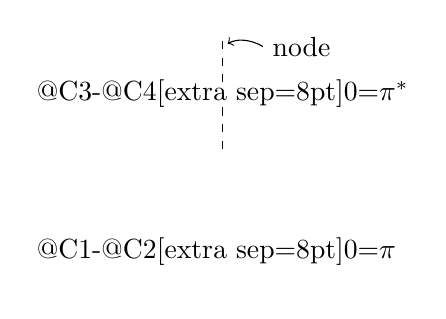
\begin{tikzpicture}
            \node at (0,2) {\chemfig{@{C3}-@{C4}\charge{[extra sep=8pt]0=$\pi^*$}{}}};
            \node          {\chemfig{@{C1}-@{C2}\charge{[extra sep=8pt]0=$\pi^{\color{white}*}$}{}}};
            \draw [dashed] (0,1.3) -- (0,2.7);
            \node (A) at (1,2.6) {node}
                (A.west) edge [bend right=30,->,shorten >=2pt] (0,2.6)
            ;
    
            \path (-1.5,-0.5) rectangle (1.5,2.5);
        \end{tikzpicture}
        \chemmove{
            \draw [thick,orx] ($(C1)+(0.0018,0)$) to[bend right=120,looseness=600] ($(C1)+(-0.0018,0)$) -- cycle;
            \filldraw [thick,draw=orx,fill=ory] ($(C1)+(0.0018,0)$) to[bend left=120,looseness=600] ($(C1)+(-0.0018,0)$) -- cycle;
            \draw [thick,orx] ($(C2)+(0.0018,0)$) to[bend right=120,looseness=600] ($(C2)+(-0.0018,0)$) -- cycle;
            \filldraw [thick,draw=orx,fill=ory] ($(C2)+(0.0018,0)$) to[bend left=120,looseness=600] ($(C2)+(-0.0018,0)$) -- cycle;
            \draw [thick,orx] ($(C3)+(0.0018,0)$) to[bend right=120,looseness=600] ($(C3)+(-0.0018,0)$) -- cycle;
            \filldraw [thick,draw=orx,fill=ory] ($(C3)+(0.0018,0)$) to[bend left=120,looseness=600] ($(C3)+(-0.0018,0)$) -- cycle;
            \filldraw [thick,draw=orx,fill=ory] ($(C4)+(0.0018,0)$) to[bend right=120,looseness=600] ($(C4)+(-0.0018,0)$) -- cycle;
            \draw [thick,orx] ($(C4)+(0.0018,0)$) to[bend left=120,looseness=600] ($(C4)+(-0.0018,0)$) -- cycle;
        }
        \caption{Nodes in $\pi$ and $\pi^*$ molecular orbitals.}
        \label{fig:piMO}
    \end{figure}
    \begin{itemize}
        \item The lower one has no nodes, because the phases are aligned left to right.
        \item The upper one has 1 node, because the phases invert left to right.
    \end{itemize}
    \item We are now ready to draw an MO diagram for the diene in Figure \ref{fig:butadieneMOs}.
    \item Diene MOs.
    \begin{figure}[h!]
        \centering
        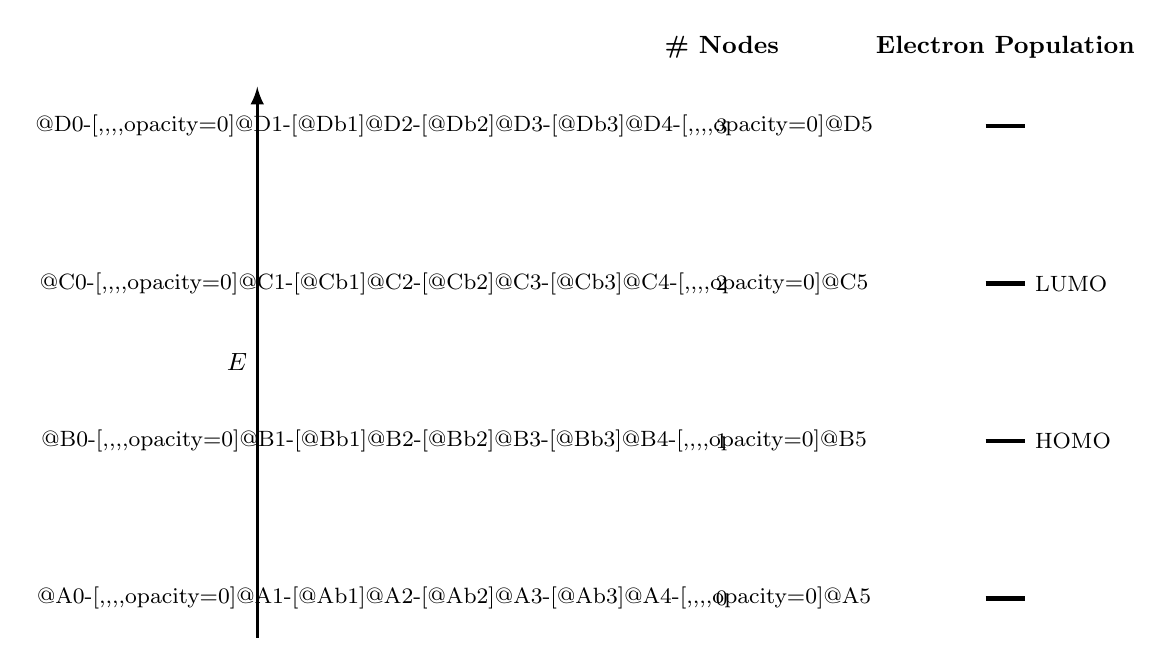
\begin{tikzpicture}
            \small
            \draw [-latex,very thick] (-2.5,-0.5) -- node[left]{$E$} (-2.5,6.5);
            \node at (3.4,7) {\textbf{\# Nodes}};
            \node at (7,7) {\textbf{Electron Population}};
    
            \footnotesize
            \node at (0,6) {\chemfig{@{D0}-[,,,,opacity=0]@{D1}-[@{Db1}]@{D2}-[@{Db2}]@{D3}-[@{Db3}]@{D4}-[,,,,opacity=0]@{D5}}};
            \node at (0,4) {\chemfig{@{C0}-[,,,,opacity=0]@{C1}-[@{Cb1}]@{C2}-[@{Cb2}]@{C3}-[@{Cb3}]@{C4}-[,,,,opacity=0]@{C5}}};
            \node at (0,2) {\chemfig{@{B0}-[,,,,opacity=0]@{B1}-[@{Bb1}]@{B2}-[@{Bb2}]@{B3}-[@{Bb3}]@{B4}-[,,,,opacity=0]@{B5}}};
            \node          {\chemfig{@{A0}-[,,,,opacity=0]@{A1}-[@{Ab1}]@{A2}-[@{Ab2}]@{A3}-[@{Ab3}]@{A4}-[,,,,opacity=0]@{A5}}};
    
            \node at (3.4,6) {3};
            \node at (3.4,4) {2};
            \node at (3.4,2) {1};
            \node at (3.4,0) {0};
    
            \draw [ultra thick]
                (6.75,6) -- ++(0.5,0)
                (6.75,4) -- ++(0.5,0) node[right]{LUMO}
                (6.75,2) -- node{\Large$\upharpoonleft\hspace{-1mm}\downharpoonright$} ++(0.5,0) node[right]{HOMO}
                (6.75,0) -- node{\Large$\upharpoonleft\hspace{-1mm}\downharpoonright$} ++(0.5,0)
            ;
        \end{tikzpicture}
        \chemmove{
            \draw [-,dashed] ([yshift=-7mm]Db3.center) -- ([yshift=7mm]Db3.center);
            \draw [-,dashed] ([yshift=-7mm]Db2.center) -- ([yshift=7mm]Db2.center);
            \draw [-,dashed] ([yshift=-7mm]Db1.center) -- ([yshift=7mm]Db1.center);
            \draw [-,dashed] ([yshift=-7mm]Cb3.center) -- ([yshift=7mm]Cb3.center);
            \draw [-,dashed] ([yshift=-7mm]Cb1.center) -- ([yshift=7mm]Cb1.center);
            \draw [-,dashed] ([yshift=-7mm]Bb2.center) -- ([yshift=7mm]Bb2.center);
            % 
            % \draw [-,pux,thick] ([xshift=-3mm]D1.center)
            %     to[bend left=85,looseness=4] (Db1.center)
            %     to[bend right=85,looseness=4] (Db2.center)
            %     to[bend left=85,looseness=4] (Db3.center)
            %     to[bend right=85,looseness=4] ([xshift=3mm]D4.center)
            % ;
            % \draw [-,pux,thick] ([xshift=-3mm]C1.center)
            %     to[bend left=85,looseness=4] (Cb1.center)
            %     to[bend right=85,looseness=2] (Cb3.center)
            %     to[bend left=85,looseness=4] ([xshift=3mm]C4.center)
            % ;
            % \draw [-,pux,thick] ([xshift=-3mm]B1.center)
            %     to[bend left=85,looseness=2] (Bb2.center)
            %     to[bend right=85,looseness=2] ([xshift=3mm]B4.center)
            % ;
            % \draw [-,pux,thick] ([xshift=-3mm]A1.center) to[bend left=85] ([xshift=3mm]A4.center);
            \draw [-,pux,thick] (D0)
                sin ([yshift=6mm]$(D0)!{1/8}!(D5)$)
                cos ($(D0)!{2/8}!(D5)$)
                sin ([yshift=-6mm]$(D0)!{3/8}!(D5)$)
                cos ($(D0)!{4/8}!(D5)$)
                sin ([yshift=6mm]$(D0)!{5/8}!(D5)$)
                cos ($(D0)!{6/8}!(D5)$)
                sin ([yshift=-6mm]$(D0)!{7/8}!(D5)$)
                cos (D5)
            ;
            \draw [-,pux,thick] (C0)
                sin ([yshift=6mm]$(C0)!{1/6}!(C5)$)
                cos ($(C0)!{2/6}!(C5)$)
                sin ([yshift=-6mm]$(C0)!{3/6}!(C5)$)
                cos ($(C0)!{4/6}!(C5)$)
                sin ([yshift=6mm]$(C0)!{5/6}!(C5)$)
                cos (C5)
            ;
            \draw [-,pux,thick] (B0)
                sin ([yshift=6mm]$(B0)!0.25!(B5)$)
                cos ($(B0)!0.5!(B5)$)
                sin ([yshift=-6mm]$(B0)!0.75!(B5)$)
                cos (B5)
            ;
            \draw [-,pux,thick] (A0)
                sin ([yshift=6mm]$(A0)!0.5!(A5)$)
                cos (A5)
            ;
            % 
            \filldraw [thick,draw=orx,fill=ory] ($(A1)+(0.0018,0)$) to[bend right=120,looseness=600] ($(A1)+(-0.0018,0)$) -- cycle;
            \draw [thick,orx] ($(A1)+(0.0018,0)$) to[bend left=120,looseness=600] ($(A1)+(-0.0018,0)$) -- cycle;
            \filldraw [thick,draw=orx,fill=ory] ($(A2)+(0.0018,0)$) to[bend right=120,looseness=600] ($(A2)+(-0.0018,0)$) -- cycle;
            \draw [thick,orx] ($(A2)+(0.0018,0)$) to[bend left=120,looseness=600] ($(A2)+(-0.0018,0)$) -- cycle;
            \filldraw [thick,draw=orx,fill=ory] ($(A3)+(0.0018,0)$) to[bend right=120,looseness=600] ($(A3)+(-0.0018,0)$) -- cycle;
            \draw [thick,orx] ($(A3)+(0.0018,0)$) to[bend left=120,looseness=600] ($(A3)+(-0.0018,0)$) -- cycle;
            \filldraw [thick,draw=orx,fill=ory] ($(A4)+(0.0018,0)$) to[bend right=120,looseness=600] ($(A4)+(-0.0018,0)$) -- cycle;
            \draw [thick,orx] ($(A4)+(0.0018,0)$) to[bend left=120,looseness=600] ($(A4)+(-0.0018,0)$) -- cycle;
            % 
            \filldraw [thick,draw=orx,fill=ory] ($(B1)+(0.0018,0)$) to[bend right=120,looseness=600] ($(B1)+(-0.0018,0)$) -- cycle;
            \draw [thick,orx] ($(B1)+(0.0018,0)$) to[bend left=120,looseness=600] ($(B1)+(-0.0018,0)$) -- cycle;
            \filldraw [thick,draw=orx,fill=ory] ($(B2)+(0.0018,0)$) to[bend right=120,looseness=600] ($(B2)+(-0.0018,0)$) -- cycle;
            \draw [thick,orx] ($(B2)+(0.0018,0)$) to[bend left=120,looseness=600] ($(B2)+(-0.0018,0)$) -- cycle;
            \draw [thick,orx] ($(B3)+(0.0018,0)$) to[bend right=120,looseness=600] ($(B3)+(-0.0018,0)$) -- cycle;
            \filldraw [thick,draw=orx,fill=ory] ($(B3)+(0.0018,0)$) to[bend left=120,looseness=600] ($(B3)+(-0.0018,0)$) -- cycle;
            \draw [thick,orx] ($(B4)+(0.0018,0)$) to[bend right=120,looseness=600] ($(B4)+(-0.0018,0)$) -- cycle;
            \filldraw [thick,draw=orx,fill=ory] ($(B4)+(0.0018,0)$) to[bend left=120,looseness=600] ($(B4)+(-0.0018,0)$) -- cycle;
            % 
            \filldraw [thick,draw=orx,fill=ory] ($(C1)+(0.0018,0)$) to[bend right=120,looseness=600] ($(C1)+(-0.0018,0)$) -- cycle;
            \draw [thick,orx] ($(C1)+(0.0018,0)$) to[bend left=120,looseness=600] ($(C1)+(-0.0018,0)$) -- cycle;
            \draw [thick,orx] ($(C2)+(0.0018,0)$) to[bend right=120,looseness=600] ($(C2)+(-0.0018,0)$) -- cycle;
            \filldraw [thick,draw=orx,fill=ory] ($(C2)+(0.0018,0)$) to[bend left=120,looseness=600] ($(C2)+(-0.0018,0)$) -- cycle;
            \draw [thick,orx] ($(C3)+(0.0018,0)$) to[bend right=120,looseness=600] ($(C3)+(-0.0018,0)$) -- cycle;
            \filldraw [thick,draw=orx,fill=ory] ($(C3)+(0.0018,0)$) to[bend left=120,looseness=600] ($(C3)+(-0.0018,0)$) -- cycle;
            \filldraw [thick,draw=orx,fill=ory] ($(C4)+(0.0018,0)$) to[bend right=120,looseness=600] ($(C4)+(-0.0018,0)$) -- cycle;
            \draw [thick,orx] ($(C4)+(0.0018,0)$) to[bend left=120,looseness=600] ($(C4)+(-0.0018,0)$) -- cycle;
            % 
            \filldraw [thick,draw=orx,fill=ory] ($(D1)+(0.0018,0)$) to[bend right=120,looseness=600] ($(D1)+(-0.0018,0)$) -- cycle;
            \draw [thick,orx] ($(D1)+(0.0018,0)$) to[bend left=120,looseness=600] ($(D1)+(-0.0018,0)$) -- cycle;
            \draw [thick,orx] ($(D2)+(0.0018,0)$) to[bend right=120,looseness=600] ($(D2)+(-0.0018,0)$) -- cycle;
            \filldraw [thick,draw=orx,fill=ory] ($(D2)+(0.0018,0)$) to[bend left=120,looseness=600] ($(D2)+(-0.0018,0)$) -- cycle;
            \filldraw [thick,draw=orx,fill=ory] ($(D3)+(0.0018,0)$) to[bend right=120,looseness=600] ($(D3)+(-0.0018,0)$) -- cycle;
            \draw [thick,orx] ($(D3)+(0.0018,0)$) to[bend left=120,looseness=600] ($(D3)+(-0.0018,0)$) -- cycle;
            \draw [thick,orx] ($(D4)+(0.0018,0)$) to[bend right=120,looseness=600] ($(D4)+(-0.0018,0)$) -- cycle;
            \filldraw [thick,draw=orx,fill=ory] ($(D4)+(0.0018,0)$) to[bend left=120,looseness=600] ($(D4)+(-0.0018,0)$) -- cycle;
        }
        \caption{Reactive molecular orbitals of a diene.}
        \label{fig:dieneMO}
    \end{figure}
    \pagebreak
    \begin{itemize}
        \item Let's start with a rule-by-rule analysis.
        \begin{enumerate}
            \item We have 4 atoms, so we draw lines for 4 MOs.
            \item The lowest energy MO in Figure \ref{fig:dieneMO} does indeed have no nodes.
            \begin{itemize}
                \item Observe that Prof. Elkin shades the top lobes first this time instead of the bottom lobes (as in Figure \ref{fig:piMO}) because the shading is arbitrary. This comment is review, but the concept is important to remember!!
            \end{itemize}
            \item For each increase in energy, we do indeed add one node.
            \begin{itemize}
                \item For the second-lowest energy level, we draw our node symmetrically right in the middle.
                \begin{itemize}
                    \item We go along shading the top (or bottom) lobes until we hit our node, and then we switch to shading the other side.
                \end{itemize}
                \item For the third-lowest energy level, we draw our nodes symmetrically as well.
                \item For the highest energy level, we draw a node between every orbital and alternate shading.
                \begin{itemize}
                    \item The highest energy level has the same alternating structure in the MOs of every conjugated $\pi$-system. For another example, see Figure \ref{fig:allylMO}.
                \end{itemize}
            \end{itemize}
        \end{enumerate}
        \item Note that we also draw (in purple) the \textbf{waveform} for every MO.
        \item Now let's populate our orbitals with electrons.
        \begin{itemize}
            \item There are four $\pi$-electrons in a diene, so per Aufbau, Pauli, and Hund, we fill the bottom two energy levels of our diagram.
            \item Filling electrons allows us to identify our HOMO and LUMO, which will be useful for justifying reactivity.
        \end{itemize}
        \item Takeaway: You probably wouldn't just guess that the LUMO (or any other MO) of a diene looks the way it does, but you can derive it using the three rules and the method of Figure \ref{fig:dieneMO}.
        \begin{itemize}
            \item Then you can use the result of your derivation to make predictions about a diene's reactivity!
            \item We'll cover such predictions next lecture.
        \end{itemize}
    \end{itemize}
    \item Why do the nodes have to be symmetric?
    \begin{itemize}
        \item Because quantum mechanics.
        \item Very simply, it has something to do with the waveform of each energy level, which you might notice mirrors the waveforms of the particle in a box.
        \item See the end of my notes for this lecture for more detail.
        \begin{itemize}
            \item Note: All extra detail on this topic is beyond the scope of this class, and will never be tested nor appear on problem sets; it is purely to satisfy your curiosity.
        \end{itemize}
    \end{itemize}
    \item An interesting finding about pericyclic reactions: They can be started by either heat ($\Delta$) or light ($h\nu$)!
    \begin{figure}[h!]
        \centering
        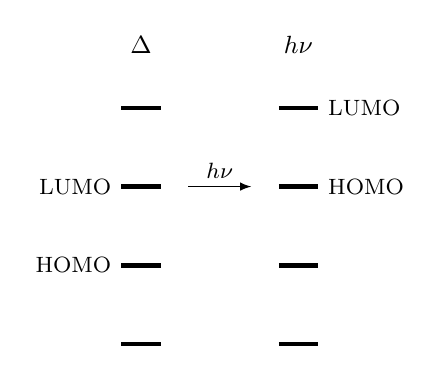
\begin{tikzpicture}
            \small
            \node at (0,3.8) {$\bm{\Delta}$};
            \node at (2,3.8) {$\bm{h\nu}$};

            \footnotesize
            \draw [ultra thick]
                (-0.25,3) -- ++(0.5,0)
                (-0.25,2) node[left]{LUMO} -- ++(0.5,0)
                (-0.25,1) node[left]{HOMO} -- node{\Large$\upharpoonleft\hspace{-1mm}\downharpoonright$} ++(0.5,0)
                (-0.25,0) -- node{\Large$\upharpoonleft\hspace{-1mm}\downharpoonright$} ++(0.5,0)
            ;
            \draw [ultra thick,xshift=2cm]
                (-0.25,3) -- ++(0.5,0) node[right]{LUMO}
                (-0.25,2) -- node{\Large$\upharpoonleft$} ++(0.5,0) node[right]{HOMO}
                (-0.25,1) -- node{\Large$\downharpoonright$} ++(0.5,0)
                (-0.25,0) -- node{\Large$\upharpoonleft\hspace{-1mm}\downharpoonright$} ++(0.5,0)
            ;
            \draw [-latex] (0.6,2) -- node[above]{$h\nu$} ++(0.8,0);
        \end{tikzpicture}
        \caption{A diene's reactive orbitals in thermal vs. photochemical pericyclic reactions.}
        \label{fig:thermPhot}
    \end{figure}
    \begin{itemize}
        \item When you think about it, heat and light are just different ways to add energy to our system so that the reaction goes.
        \item Indeed, pericyclic reactions are cool because you don't have to add a chemical reagent to make one go; rather, you just heat it up or shine light at it, and it reacts away!
        \item How do photochemical reactions work?
        \begin{itemize}
            \item When light is absorbed, one electron is excited from the HOMO to the LUMO, and none of the spins of \emph{any} of the electrons change (Figure \ref{fig:thermPhot}).
            \begin{itemize}
                \item There's a lot more photophysics here that you can go into, but that's beyond the scope of this course.
            \end{itemize}
            \item Such excitation is important because it gives us a new HOMO and a new LUMO.
            \begin{itemize}
                \item These new reactive orbitals have important consequences that we'll discuss later, especially for the stereochemistry of the product.
            \end{itemize}
        \end{itemize}
    \end{itemize}
    \item Let's now look at the MOs of one more conjugated system.
    \item Allyl MOs.
    \begin{figure}[h!]
        \centering
        \begin{tikzpicture}
            \setcharge{extra sep=5pt}
            \small
            \draw [-latex,very thick] (-2.5,-0.5) -- node[left]{$E$} (-2.5,4.5);
            \node at (3.5,5) {\chemfig[atom sep=1.4em]{=_[:30]-[:-30]\charge{0=$\oplus$}{}}};
            \node at (7,5) {\chemfig[atom sep=1.4em]{=_[:30]-[:-30]\charge{[extra sep=3pt]0=\.}{}}};
            \node at (10.5,5) {\chemfig[atom sep=1.4em]{=_[:30]-[:-30]\charge{0=$\ominus$}{}}};
    
            \footnotesize
            \node at (0,4) {\chemfig{@{C1}-[@{Cb1}]@{C2}-[@{Cb2}]@{C3}}};
            \node at (0,2) {\chemfig{@{B1}-[@{Bb1}]@{B2}-[@{Bb2}]@{B3}}};
            \node          {\chemfig{@{A1}-[@{Ab1}]@{A2}-[@{Ab2}]@{A3}}};
    
            \draw [ultra thick,xshift=-3.5cm]
                (6.75,4) -- ++(0.5,0)
                (6.75,2) -- ++(0.5,0) node[right]{LUMO}
                (6.75,0) -- node{\Large$\upharpoonleft\hspace{-1mm}\downharpoonright$} ++(0.5,0)
            ;
            \draw [ultra thick]
                (6.75,4) -- ++(0.5,0)
                (6.75,2) -- node{\Large$\upharpoonleft$} ++(0.5,0) node[right]{SOMO}
                (6.75,0) -- node{\Large$\upharpoonleft\hspace{-1mm}\downharpoonright$} ++(0.5,0)
            ;
            \draw [ultra thick,xshift=3.5cm]
                (6.75,4) -- ++(0.5,0)
                (6.75,2) -- node{\Large$\upharpoonleft\hspace{-1mm}\downharpoonright$} ++(0.5,0) node[right]{HOMO}
                (6.75,0) -- node{\Large$\upharpoonleft\hspace{-1mm}\downharpoonright$} ++(0.5,0)
            ;
        \end{tikzpicture}
        \chemmove{
            \draw [-,dashed] ([yshift=-7mm]Cb2.center) -- ([yshift=7mm]Cb2.center);
            \draw [-,dashed] ([yshift=-7mm]Cb1.center) -- ([yshift=7mm]Cb1.center);
            \draw [-,dashed] ([yshift=-7mm]B2.center) -- ([yshift=7mm]B2.center);
            % 
            \filldraw [thick,draw=orx,fill=ory] ($(C1)+(0.0018,0)$) to[bend right=120,looseness=600] ($(C1)+(-0.0018,0)$) -- cycle;
            \draw [thick,orx] ($(C1)+(0.0018,0)$) to[bend left=120,looseness=600] ($(C1)+(-0.0018,0)$) -- cycle;
            \draw [thick,orx] ($(C2)+(0.0018,0)$) to[bend right=120,looseness=600] ($(C2)+(-0.0018,0)$) -- cycle;
            \filldraw [thick,draw=orx,fill=ory] ($(C2)+(0.0018,0)$) to[bend left=120,looseness=600] ($(C2)+(-0.0018,0)$) -- cycle;
            \filldraw [thick,draw=orx,fill=ory] ($(C3)+(0.0018,0)$) to[bend right=120,looseness=600] ($(C3)+(-0.0018,0)$) -- cycle;
            \draw [thick,orx] ($(C3)+(0.0018,0)$) to[bend left=120,looseness=600] ($(C3)+(-0.0018,0)$) -- cycle;
            % 
            \filldraw [thick,draw=orx,fill=ory] ($(B1)+(0.0018,0)$) to[bend right=120,looseness=600] ($(B1)+(-0.0018,0)$) -- cycle;
            \draw [thick,orx] ($(B1)+(0.0018,0)$) to[bend left=120,looseness=600] ($(B1)+(-0.0018,0)$) -- cycle;
            \draw [thick,orx] ($(B3)+(0.0018,0)$) to[bend right=120,looseness=600] ($(B3)+(-0.0018,0)$) -- cycle;
            \filldraw [thick,draw=orx,fill=ory] ($(B3)+(0.0018,0)$) to[bend left=120,looseness=600] ($(B3)+(-0.0018,0)$) -- cycle;
            % 
            \filldraw [thick,draw=orx,fill=ory] ($(A1)+(0.0018,0)$) to[bend right=120,looseness=600] ($(A1)+(-0.0018,0)$) -- cycle;
            \draw [thick,orx] ($(A1)+(0.0018,0)$) to[bend left=120,looseness=600] ($(A1)+(-0.0018,0)$) -- cycle;
            \filldraw [thick,draw=orx,fill=ory] ($(A2)+(0.0018,0)$) to[bend right=120,looseness=600] ($(A2)+(-0.0018,0)$) -- cycle;
            \draw [thick,orx] ($(A2)+(0.0018,0)$) to[bend left=120,looseness=600] ($(A2)+(-0.0018,0)$) -- cycle;
            \filldraw [thick,draw=orx,fill=ory] ($(A3)+(0.0018,0)$) to[bend right=120,looseness=600] ($(A3)+(-0.0018,0)$) -- cycle;
            \draw [thick,orx] ($(A3)+(0.0018,0)$) to[bend left=120,looseness=600] ($(A3)+(-0.0018,0)$) -- cycle;
        }
        \caption{Reactive molecular orbitals of an allyl group.}
        \label{fig:allylMO}
    \end{figure}
    \begin{itemize}
        \item Let's do another rule-by-rule analysis.
        \begin{enumerate}
            \item Three atoms going in means three MOs.
            \item Shade all the same phases in the bottom MO.
            \item Add nodes for the upper orbitals.
            \begin{itemize}
                \item Put your node right in the middle for the middle MO.
                \begin{itemize}
                    \item It has to be symmetric!
                    \item Every time you have an odd number of atoms, some $p$-orbital will get deleted like this.
                \end{itemize}
                \item For the top MO, once again do everything alternating.
            \end{itemize}
        \end{enumerate}
        \item Note that we have not yet specified whether this is an allyl cation, allyl radical, or allyl anion!
        \item We will have a different number of electrons for all three species (even though we have the same MOs), so let's fill electrons for each of these species.
        \begin{itemize}
            \item Allyl cation: Two electrons, so fill just the bottom MO.
            \begin{itemize}
                \item Like any carbocation, the allyl cation will react as an electrophile.
                \item If it reacts as an electrophile, it must react with its LUMO (which is the middle orbital).
            \end{itemize}
            \item Allyl radical: Three electrons, so fill the bottom MO and start filling the middle MO.
            \begin{itemize}
                \item Like any radical, the allyl radical reacts as a\dots well\dots radical.
                \item If it reacts as a radical, it must react with its \textbf{SOMO} (also the middle orbital).
            \end{itemize}
            \pagebreak
            \item Allyl anion: Four electrons, so fill the bottom and middle MOs.
            \begin{itemize}
                \item Like any carbanion, the allyl anion will react as a nucleophile.
                \item If it reacts as a nucleophile, it must react with its HOMO (still the middle orbital!).
            \end{itemize}
        \end{itemize}
        \item Interesting consequence of this filling: All three allyl species should only react with their middle-energy MO!
        \begin{itemize}
            \item This would predict that all allyl reactivity occurs at the termini of the allyl group, not the middle carbon, since all of the density of the middle orbital is at the termini and none of it is at the middle carbon.
            \item This prediction is experimentally confirmed!
        \end{itemize}
    \end{itemize}
    \item \textbf{Singly occupied molecular orbital}: The molecular orbital in which an unpaired radical electron exists. \emph{Also known as} \textbf{SOMO}.
    \item An elaboration on why nodes must be placed symmetrically in the MOs of conjugated $\pi$-systems (see Figures \ref{fig:dieneMO} and \ref{fig:allylMO} and the associated discussion).
    \begin{itemize}
        \item Reminder: Everything from here, on, in these notes is beyond the scope of this class!
        \item The long-short.
        \begin{itemize}
            \item The waveforms in Figure \ref{fig:dieneMO} are \emph{exactly} equal to their corresponding particle-in-a-box wave functions (according to some analyses of quantum mechanics).
            \begin{itemize}
                \item This relationship can be rationalized intuitively because a conjugated $\pi$-system is like an extended, one-dimensional box in which a quantum particle (namely, an electron) lives.
            \end{itemize}
            \item The implication is that the molecular orbitals of a conjugated $\pi$-system look \emph{exactly} like the particle-in-a-box orbitals, including having nodes in the same places.
            \item This actually also means that the individual $p$-orbitals making up the MOs are different sizes!
            \begin{itemize}
                \item For example, in the lowest energy MO in Figure \ref{fig:dieneMO}, the two middle $p$-orbitals will be larger than the two terminal $p$-orbitals.
                \item More relevantly, the HOMO and LUMO in Figure \ref{fig:dieneMO} will have larger terminal $p$-orbitals, which explains why dienes react at their ends and not in the middle; we have already seen an example of dienes reacting at their terminal carbons instead of their middle carbons in Figure \ref{fig:dielsAlder}.
            \end{itemize}
        \end{itemize}
        \item More detail.
        \begin{itemize}
            \item The exact sizes of each $p$-orbital in a given MO of a conjugated $\pi$-system can be calculated --- by hand --- using only linear algebra. This calculation is part of something called \textbf{H\"{u}ckel theory}.
            \item You can learn about H\"{u}ckel theory by taking a course in quantum mechanics, inorganic chemistry, or graduate physical organic chemistry.
        \end{itemize}
        \item If you are interested in reading more about this now, look through the attached PDF. I'd recommend starting with the diagrams and sine/cosine functions on pages 6.6 and 6.7. Enjoy!
    \end{itemize}
\end{itemize}

% 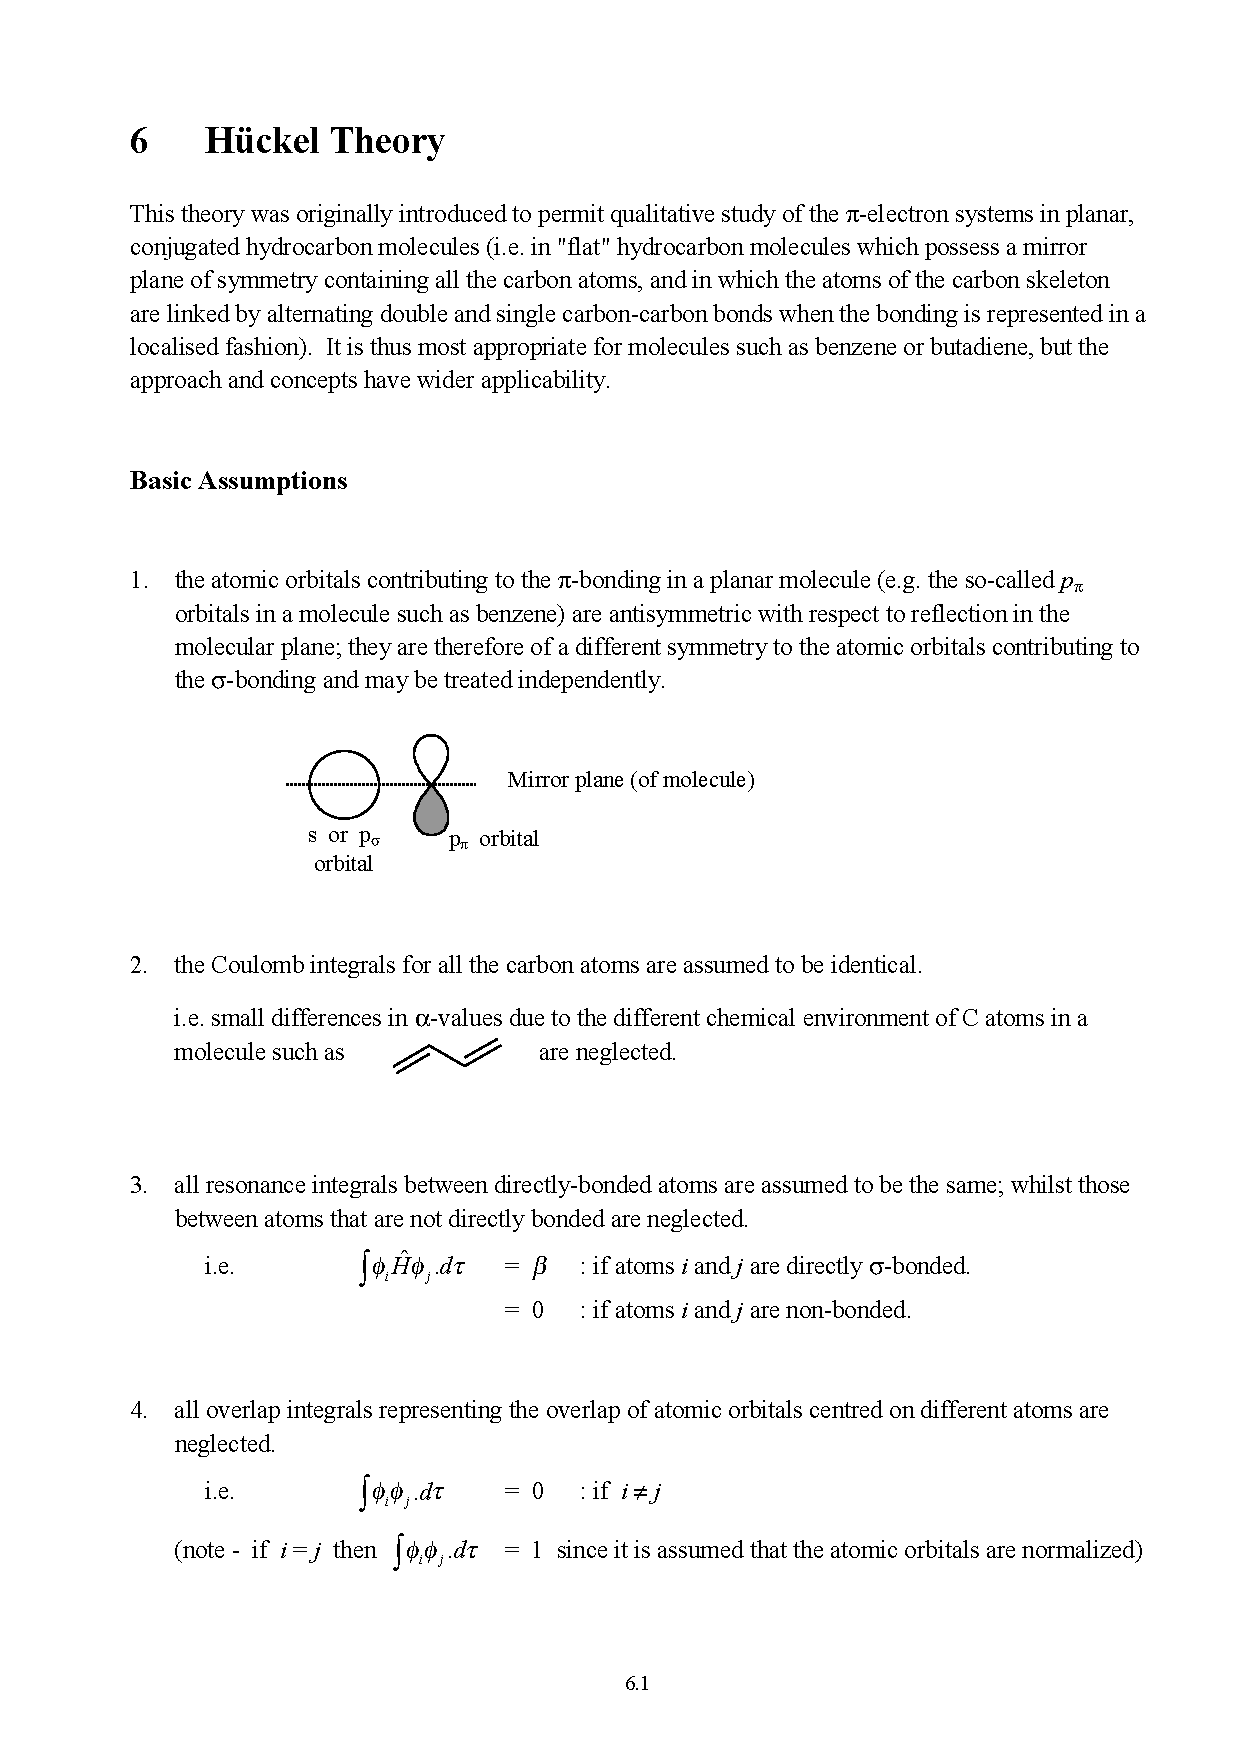
\includepdf[pages=-]{BlackboardPics/L12/WhySymmetricNodes.pdf}



\section{Diels-Alder - 1}
\begin{itemize}
    \item \marginnote{10/4:}Lecture 12 recap.
    \begin{itemize}
        \item Periyclic reactions have concerted and cyclics transition states.
        \begin{itemize}
            \item Essentially, what unites all of these reactions is that they have electron arrows moving in a ring!
        \end{itemize}
        \item All of these reactions are theoretically reversible.
        \item Prof. Elkin redraws the prototypical pericyclic reactions from last class.
        \pagebreak
        \item Three main classes.
        \begin{enumerate}
            \item Cycloaddition.
            \begin{itemize}
                \item Bond types changed: \ce{$2\pi$ <=> $2\sigma$}.
                \item Nomenclature: $[m+n]$.
                \item General form: See Figure \ref{fig:dielsAlder}.
                \begin{itemize}
                    \item To reiterate: This reaction can also proceed in reverse, i.e., from right to left!
                \end{itemize}
            \end{itemize}
            \item Electrocyclization.
            \begin{itemize}
                \item Bond types changed: \ce{$1\pi$ <=> $1\sigma$}.
                \item Nomenclature: $m\pi$.
                \item General form: See Figure \ref{fig:electrocyc6p}.
                \begin{itemize}
                    \item To reiterate: This reaction can also proceed in reverse, i.e., from right to left!
                \end{itemize}
            \end{itemize}
            \item Sigmatropic rearrangements.
            \begin{itemize}
                \item Bonds moved: $1\sigma$.
                \item Nomenclature: $[m,n]$.
                \item General form: See Figure \ref{fig:sigmatrop15}.
                \begin{itemize}
                    \item To reiterate: This reaction can also proceed in reverse, i.e., from right to left!
                \end{itemize}
            \end{itemize}
        \end{enumerate}
    \end{itemize}
    \item Announcements.
    \begin{itemize}
        \item Please fill out the feedback survey in Canvas $>$ Announcements.
        \item PSet 3 is due today.
        \item PSet 4 will be posted today.
        \begin{itemize}
            \item It is the last PSet before Exam 2.
            \item It only covers Diels-Alder content. However, the rest of this unit's content (cycloadditions, electrocyclizations, and sigmatropic rearrangements) \emph{will} be on Exam 2 as well.
            \item So to prepare for the exam, continue doing the Recitation Worksheets even after PSet 4!!
        \end{itemize}
    \end{itemize}
    \item Today: Diels-Alder (lecture 1 of 2).
    \item Recall from last lecture that a \emph{Diels-Alder reaction} is a $[4+2]$ cycloaddition.
    \begin{itemize}
        \item Specifically, a \textbf{diene} reacts with an olefin, which we call the \textbf{dienophile}.
        \item The simplest Diels-Alder (DA) reaction is drawn in Figure \ref{fig:dielsAlder}.
        \begin{itemize}
            \item This is actually a terrible Diels-Alder reaction because there's a poor HOMO-LUMO energy match (we'll talk more about what that means shortly).
        \end{itemize}
        \item The Diels-Alder is a powerful tool to make six-membered rings.
        \begin{itemize}
            \item We see a lot of six-membered rings in organic chemistry, so the Diels-Alder is very useful.
        \end{itemize}
        \item This reaction is very predictible: It is \textbf{regioselective}, \textbf{stereospecific}, and \textbf{reliable}.\footnote{We'll discuss both regioselectivity and stereospecificity later this lecture, and stereospecificity even further on Monday.}
    \end{itemize}
    \item \textbf{Diene}: A compound that contains two conjugated double bonds.
    \begin{itemize}
        \item The diene is (usually) the HOMO.
        \item You can think of it as the nucleophile.
    \end{itemize}
    \item \textbf{Dienophile}: An olefin. \emph{Etymology} from Latin "lover of dienes."
    \begin{itemize}
        \item The dienophile is (usually) the LUMO.
        \item You can think of it as the electrophile.
    \end{itemize}
    \item \textbf{Reliable} (reaction): A reaction that almost always works if you have the right energy matching.
    \item Let's look at the MO picture for a Diels-Alder reaction.
    \begin{figure}[H]
        \centering
        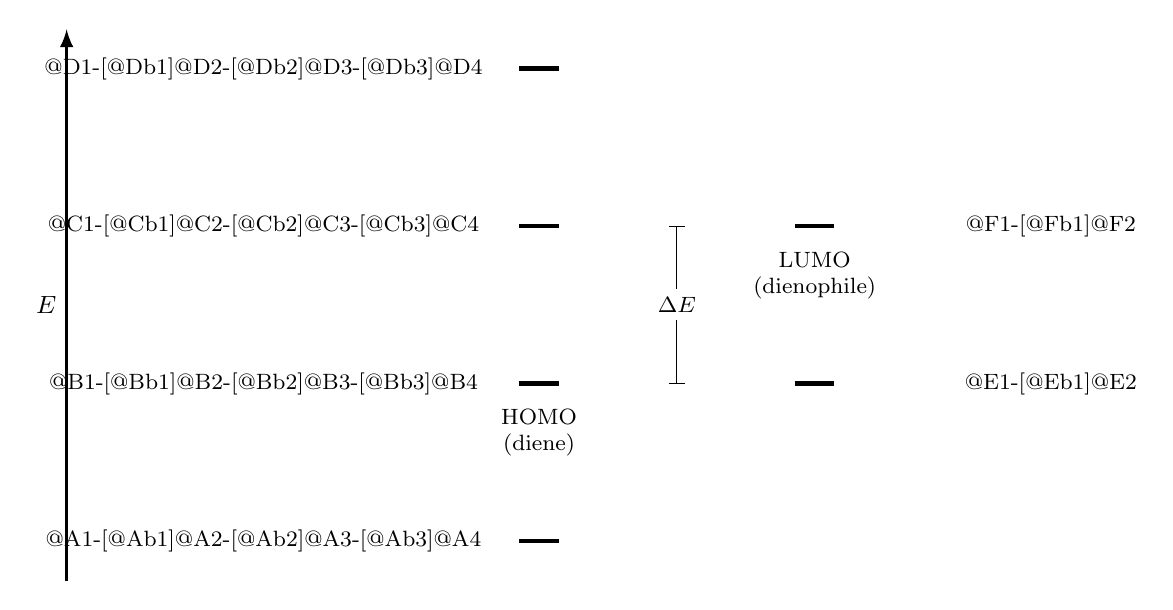
\begin{tikzpicture}
            \small
            \draw [-latex,very thick] (-2.5,-0.5) -- node[left]{$E$} (-2.5,6.5);
    
            \footnotesize
            \node at (0,6) {\chemfig{@{D1}-[@{Db1}]@{D2}-[@{Db2}]@{D3}-[@{Db3}]@{D4}}};
            \node at (0,4) {\chemfig{@{C1}-[@{Cb1}]@{C2}-[@{Cb2}]@{C3}-[@{Cb3}]@{C4}}};
            \node at (0,2) {\chemfig{@{B1}-[@{Bb1}]@{B2}-[@{Bb2}]@{B3}-[@{Bb3}]@{B4}}};
            \node          {\chemfig{@{A1}-[@{Ab1}]@{A2}-[@{Ab2}]@{A3}-[@{Ab3}]@{A4}}};
    
            \node at (10,4) {\chemfig{@{F1}-[@{Fb1}]@{F2}}};
            \node at (10,2) {\chemfig{@{E1}-[@{Eb1}]@{E2}}};
    
            \draw [ultra thick]
                (3.25,6) -- ++(0.5,0)
                (3.25,4) -- ++(0.5,0)
                (3.25,2) -- node{\Large$\upharpoonleft\hspace{-1mm}\downharpoonright$} node[below=2mm,align=center]{HOMO\\(diene)} ++(0.5,0)
                (3.25,0) -- node{\Large$\upharpoonleft\hspace{-1mm}\downharpoonright$} ++(0.5,0)
            ;
            \draw [ultra thick,xshift=3.5cm]
                (3.25,4) -- node[below=2mm,align=center]{LUMO\\(dienophile)} ++(0.5,0)
                (3.25,2) -- node{\Large$\upharpoonleft\hspace{-1mm}\downharpoonright$} ++(0.5,0)
            ;
    
            % \draw [curved arrow={8pt}{4pt},-{Stealth[round,scale=1.1,inset'=0pt 0.55]}] (3.5,2) to[out=60,in=120] (7,4);
            \draw [|-|] (5.25,2) -- node[fill=white,inner sep=1mm]{$\Delta E$} (5.25,4);
        \end{tikzpicture}
        \chemmove{
            \draw [-,dashed] ([yshift=-7mm]Db3.center) -- ([yshift=7mm]Db3.center);
            \draw [-,dashed] ([yshift=-7mm]Db2.center) -- ([yshift=7mm]Db2.center);
            \draw [-,dashed] ([yshift=-7mm]Db1.center) -- ([yshift=7mm]Db1.center);
            \draw [-,dashed] ([yshift=-7mm]Cb3.center) -- ([yshift=7mm]Cb3.center);
            \draw [-,dashed] ([yshift=-7mm]Cb1.center) -- ([yshift=7mm]Cb1.center);
            \draw [-,dashed] ([yshift=-7mm]Bb2.center) -- ([yshift=7mm]Bb2.center);
            % 
            \draw [-,dashed] ([yshift=-7mm]Fb1.center) -- ([yshift=7mm]Fb1.center);
            % 
            \filldraw [thick,draw=orx,fill=ory] ($(A1)+(0.0018,0)$) to[bend right=120,looseness=600] ($(A1)+(-0.0018,0)$) -- cycle;
            \draw [thick,orx] ($(A1)+(0.0018,0)$) to[bend left=120,looseness=600] ($(A1)+(-0.0018,0)$) -- cycle;
            \filldraw [thick,draw=orx,fill=ory] ($(A2)+(0.0018,0)$) to[bend right=120,looseness=600] ($(A2)+(-0.0018,0)$) -- cycle;
            \draw [thick,orx] ($(A2)+(0.0018,0)$) to[bend left=120,looseness=600] ($(A2)+(-0.0018,0)$) -- cycle;
            \filldraw [thick,draw=orx,fill=ory] ($(A3)+(0.0018,0)$) to[bend right=120,looseness=600] ($(A3)+(-0.0018,0)$) -- cycle;
            \draw [thick,orx] ($(A3)+(0.0018,0)$) to[bend left=120,looseness=600] ($(A3)+(-0.0018,0)$) -- cycle;
            \filldraw [thick,draw=orx,fill=ory] ($(A4)+(0.0018,0)$) to[bend right=120,looseness=600] ($(A4)+(-0.0018,0)$) -- cycle;
            \draw [thick,orx] ($(A4)+(0.0018,0)$) to[bend left=120,looseness=600] ($(A4)+(-0.0018,0)$) -- cycle;
            % 
            \filldraw [thick,draw=orx,fill=ory] ($(B1)+(0.0018,0)$) to[bend right=120,looseness=600] ($(B1)+(-0.0018,0)$) -- cycle;
            \draw [thick,orx] ($(B1)+(0.0018,0)$) to[bend left=120,looseness=600] ($(B1)+(-0.0018,0)$) -- cycle;
            \filldraw [thick,draw=orx,fill=ory] ($(B2)+(0.0018,0)$) to[bend right=120,looseness=600] ($(B2)+(-0.0018,0)$) -- cycle;
            \draw [thick,orx] ($(B2)+(0.0018,0)$) to[bend left=120,looseness=600] ($(B2)+(-0.0018,0)$) -- cycle;
            \draw [thick,orx] ($(B3)+(0.0018,0)$) to[bend right=120,looseness=600] ($(B3)+(-0.0018,0)$) -- cycle;
            \filldraw [thick,draw=orx,fill=ory] ($(B3)+(0.0018,0)$) to[bend left=120,looseness=600] ($(B3)+(-0.0018,0)$) -- cycle;
            \draw [thick,orx] ($(B4)+(0.0018,0)$) to[bend right=120,looseness=600] ($(B4)+(-0.0018,0)$) -- cycle;
            \filldraw [thick,draw=orx,fill=ory] ($(B4)+(0.0018,0)$) to[bend left=120,looseness=600] ($(B4)+(-0.0018,0)$) -- cycle;
            % 
            \filldraw [thick,draw=orx,fill=ory] ($(C1)+(0.0018,0)$) to[bend right=120,looseness=600] ($(C1)+(-0.0018,0)$) -- cycle;
            \draw [thick,orx] ($(C1)+(0.0018,0)$) to[bend left=120,looseness=600] ($(C1)+(-0.0018,0)$) -- cycle;
            \draw [thick,orx] ($(C2)+(0.0018,0)$) to[bend right=120,looseness=600] ($(C2)+(-0.0018,0)$) -- cycle;
            \filldraw [thick,draw=orx,fill=ory] ($(C2)+(0.0018,0)$) to[bend left=120,looseness=600] ($(C2)+(-0.0018,0)$) -- cycle;
            \draw [thick,orx] ($(C3)+(0.0018,0)$) to[bend right=120,looseness=600] ($(C3)+(-0.0018,0)$) -- cycle;
            \filldraw [thick,draw=orx,fill=ory] ($(C3)+(0.0018,0)$) to[bend left=120,looseness=600] ($(C3)+(-0.0018,0)$) -- cycle;
            \filldraw [thick,draw=orx,fill=ory] ($(C4)+(0.0018,0)$) to[bend right=120,looseness=600] ($(C4)+(-0.0018,0)$) -- cycle;
            \draw [thick,orx] ($(C4)+(0.0018,0)$) to[bend left=120,looseness=600] ($(C4)+(-0.0018,0)$) -- cycle;
            % 
            \filldraw [thick,draw=orx,fill=ory] ($(D1)+(0.0018,0)$) to[bend right=120,looseness=600] ($(D1)+(-0.0018,0)$) -- cycle;
            \draw [thick,orx] ($(D1)+(0.0018,0)$) to[bend left=120,looseness=600] ($(D1)+(-0.0018,0)$) -- cycle;
            \draw [thick,orx] ($(D2)+(0.0018,0)$) to[bend right=120,looseness=600] ($(D2)+(-0.0018,0)$) -- cycle;
            \filldraw [thick,draw=orx,fill=ory] ($(D2)+(0.0018,0)$) to[bend left=120,looseness=600] ($(D2)+(-0.0018,0)$) -- cycle;
            \filldraw [thick,draw=orx,fill=ory] ($(D3)+(0.0018,0)$) to[bend right=120,looseness=600] ($(D3)+(-0.0018,0)$) -- cycle;
            \draw [thick,orx] ($(D3)+(0.0018,0)$) to[bend left=120,looseness=600] ($(D3)+(-0.0018,0)$) -- cycle;
            \draw [thick,orx] ($(D4)+(0.0018,0)$) to[bend right=120,looseness=600] ($(D4)+(-0.0018,0)$) -- cycle;
            \filldraw [thick,draw=orx,fill=ory] ($(D4)+(0.0018,0)$) to[bend left=120,looseness=600] ($(D4)+(-0.0018,0)$) -- cycle;
            % 
            \filldraw [thick,draw=orx,fill=ory] ($(E1)+(0.0018,0)$) to[bend right=120,looseness=600] ($(E1)+(-0.0018,0)$) -- cycle;
            \draw [thick,orx] ($(E1)+(0.0018,0)$) to[bend left=120,looseness=600] ($(E1)+(-0.0018,0)$) -- cycle;
            \filldraw [thick,draw=orx,fill=ory] ($(E2)+(0.0018,0)$) to[bend right=120,looseness=600] ($(E2)+(-0.0018,0)$) -- cycle;
            \draw [thick,orx] ($(E2)+(0.0018,0)$) to[bend left=120,looseness=600] ($(E2)+(-0.0018,0)$) -- cycle;
            % 
            \filldraw [thick,draw=orx,fill=ory] ($(F1)+(0.0018,0)$) to[bend right=120,looseness=600] ($(F1)+(-0.0018,0)$) -- cycle;
            \draw [thick,orx] ($(F1)+(0.0018,0)$) to[bend left=120,looseness=600] ($(F1)+(-0.0018,0)$) -- cycle;
            \draw [thick,orx] ($(F2)+(0.0018,0)$) to[bend right=120,looseness=600] ($(F2)+(-0.0018,0)$) -- cycle;
            \filldraw [thick,draw=orx,fill=ory] ($(F2)+(0.0018,0)$) to[bend left=120,looseness=600] ($(F2)+(-0.0018,0)$) -- cycle;
        }
        \caption{Reactive molecular orbitals in a Diels-Alder.}
        \label{fig:DAMO}
    \end{figure}
    \begin{itemize}
        \item Recall our diene MOs from last lecture (Figure \ref{fig:dieneMO}).\footnote{Prof. Elkin reviews the three rules for drawing the MOs of conjugated systems; remember these!!}
        \begin{itemize}
            \item Specifically, recall that our HOMO has the orbital picture of the second energy level. Since we have said that the diene reacts with its HOMO, this is the important orbital to watch.
        \end{itemize}
        \item Recall also our dienophile MOs from last lecture (Figure \ref{fig:piMO}).
        \begin{itemize}
            \item The olefin has two electrons, so its LUMO is the second energy level. Since we have said that the dienophile reacts with its LUMO, this is the important orbital to watch.
        \end{itemize}
        \item Initially, we have a poor energy match between HOMO and LUMO ($\Delta E$ is large). Therefore, if we want to improve the reaction, we should strive to bring their energies closer together.
        \item Two main things to accomplish this goal of bringing HOMO and LUMO energies closer together.
        \begin{enumerate}
            \item Raise the HOMO by adding EDGs to the diene.
            \item Lower the LUMO by adding EWGs to the dienophile.
        \end{enumerate}
    \end{itemize}
    \item Example: A Diels-Alder reaction that does work well.
    \begin{figure}[h!]
        \centering
        \footnotesize
        \begin{subfigure}[b]{0.3\linewidth}
            \centering
            \begin{tikzpicture}
                \draw [xscale=2,rotate=-23]
                    (90:1.1) node[above right=-2pt]{\ce{OMe}} -- (90:0.6) coordinate (B1) -- (150:0.6) coordinate (B2) -- (210:0.6) coordinate (B3) -- (270:0.6) coordinate (B4)
                    (90:0.53) -- (150:0.53) (210:0.53) -- (270:0.53)
                ;
                \draw [xshift=2mm,yshift=-1.5cm,xscale=2,rotate=-23]
                    (0,-0.5) coordinate (F1) -- (0,0.5) coordinate (F2) -- ++(30:0.4) node[right]{\ce{CO2Me}}
                    (0.06,-0.5) -- (0.06,0.45)
                ;
                \draw [dashed]
                    (B1) -- (F2)
                    (B4) -- (F1)
                ;
    
                \draw [thick,opacity=0] ($(F1)+(0.0018,0)$) to[bend left=120,looseness=600] ($(F1)+(-0.0018,0)$) -- cycle;
            \end{tikzpicture}
            \caption{Reactants.}
            \label{fig:DAorb3Da}
        \end{subfigure}
        \begin{subfigure}[b]{0.3\linewidth}
            \centering
            \begin{tikzpicture}
                \draw [xscale=2,rotate=-23]
                    (90:1.1) node[above right=-2pt]{\ce{OMe}} -- (90:0.6) coordinate (B1) -- (150:0.6) coordinate (B2) -- (210:0.6) coordinate (B3) -- (270:0.6) coordinate (B4)
                ;
                \draw [xshift=2mm,yshift=-1.5cm,xscale=2,rotate=-23]
                    (0,-0.5) coordinate (F1) -- (0,0.5) coordinate (F2) -- ++(30:0.4) node[right]{\ce{CO2Me}}
                ;
    
                \filldraw [thick,draw=orx,fill=ory] ($(B1)+(0.0018,0)$) to[bend right=120,looseness=600] ($(B1)+(-0.0018,0)$) -- cycle;
                \draw [thick,orx] ($(B1)+(0.0018,0)$) to[bend left=120,looseness=600] ($(B1)+(-0.0018,0)$) -- cycle;
                \filldraw [thick,draw=orx,fill=ory] ($(B2)+(0.0018,0)$) to[bend right=120,looseness=600] ($(B2)+(-0.0018,0)$) -- cycle;
                \draw [thick,orx] ($(B2)+(0.0018,0)$) to[bend left=120,looseness=600] ($(B2)+(-0.0018,0)$) -- cycle;
                \draw [thick,orx] ($(B3)+(0.0018,0)$) to[bend right=120,looseness=600] ($(B3)+(-0.0018,0)$) -- cycle;
                \filldraw [thick,draw=orx,fill=ory] ($(B3)+(0.0018,0)$) to[bend left=120,looseness=600] ($(B3)+(-0.0018,0)$) -- cycle;
                \draw [thick,orx] ($(B4)+(0.0018,0)$) to[bend right=120,looseness=600] ($(B4)+(-0.0018,0)$) -- cycle;
                \filldraw [thick,draw=orx,fill=ory] ($(B4)+(0.0018,0)$) to[bend left=120,looseness=600] ($(B4)+(-0.0018,0)$) -- cycle;
    
                \filldraw [thick,draw=orx,fill=ory] ($(F1)+(0.0018,0)$) to[bend right=120,looseness=600] ($(F1)+(-0.0018,0)$) -- cycle;
                \draw [thick,orx] ($(F1)+(0.0018,0)$) to[bend left=120,looseness=600] ($(F1)+(-0.0018,0)$) -- cycle;
                \draw [thick,orx] ($(F2)+(0.0018,0)$) to[bend right=120,looseness=600] ($(F2)+(-0.0018,0)$) -- cycle;
                \filldraw [thick,draw=orx,fill=ory] ($(F2)+(0.0018,0)$) to[bend left=120,looseness=600] ($(F2)+(-0.0018,0)$) -- cycle;
    
                \draw [cyan,thick] ([xshift=-1mm,yshift=-6mm]B4) to[bend right=20] ([xshift=-2mm,yshift=4mm]F1);
                \draw [cyan,thick] ([xshift=1.5mm,yshift=-5mm]B1) to[bend left=20] ([xshift=1mm,yshift=6mm]F2);
            \end{tikzpicture}
            \caption{Reactant orbitals.}
            \label{fig:DAorb3Db}
        \end{subfigure}
        \begin{subfigure}[b]{0.3\linewidth}
            \centering
            \begin{tikzpicture}
                \draw [xscale=2,rotate=-23]
                    (90:1.1) node[above right=-2pt]{\ce{OMe}} -- (90:0.6) coordinate (B1) -- (150:0.6) coordinate (B2) -- (210:0.6) coordinate (B3) -- (270:0.6) coordinate (B4)
                ;
                \draw [xshift=0mm,yshift=-1cm,xscale=2,rotate=-23]
                    (0,-0.6) coordinate (F1) -- (0,0.6) coordinate (F2) -- ++(30:0.4) node[right]{\ce{CO2Me}}
                ;
    
                \filldraw [thick,draw=orx,fill=ory] ($(B1)+(0.0018,0)$) to[bend right=130,looseness=600] ($(B1)+(-0.0018,0)$) -- cycle;
                \draw [thick,orx] ($(B4)+(0.0018,0)$) to[bend right=130,looseness=600] ($(B4)+(-0.0018,0)$) -- cycle;
    
                \draw [thick,orx] ($(F1)+(0.0018,0)$) to[bend left=130,looseness=600] ($(F1)+(-0.0018,0)$) -- cycle;
                \filldraw [thick,draw=orx,fill=ory] ($(F2)+(0.0018,0)$) to[bend left=130,looseness=600] ($(F2)+(-0.0018,0)$) -- cycle;
    
                \filldraw [thick,draw=orx,fill=ory] ($(B4)!0.5!(F1)$) ellipse (1.8mm and 5mm);
                \draw [thick,orx] ($(B1)!0.5!(F2)$) ellipse (1.8mm and 5mm);
    
                \path (0,0) -- (0,-2.4);
            \end{tikzpicture}
            \caption{Product orbitals.}
            \label{fig:DAorb3Dc}
        \end{subfigure}
        \caption{Diels-Alder orbitals in 3D space.}
        \label{fig:DAorb3D}
    \end{figure}
    \pagebreak
    \begin{itemize}
        \item Let's analyze the new reactants we've drawn (Figure \ref{fig:DAorb3Da}).
        \begin{itemize}
            \item The methoxy-substituted diene is a better nucleophile than 1,3-butadiene because methoxy groups are electron-donating.
            \item The ester-substituted dienophile is a better electrophile than ethylene because ester groups are electron-withdrawing.
            \item Recall electrophilic aromatic substitution reactions, which tell you what substitutents are electron donating vs. withdrawing. Review this 5.12 content!!
        \end{itemize}
        \item Now let's look at their orbitals (Figure \ref{fig:DAorb3Db}).
        \begin{itemize}
            \item We draw a "perspective picture" of the HOMO and LUMO.
            \item Observe that the phases of the HOMO and LUMO match!
            \begin{itemize}
                \item Specifically, we mean that the lobes connected by the blue lines have the same shading.
            \end{itemize}
            \item A note on shading.
            \begin{itemize}
                \item The \emph{relative} shading between reacting molecules \emph{does} matter because we've got to see overlap between pairs of shaded lobes and pairs of unshaded lobes when we're forming bonds.
                \item Thus, while we could invert the shading of every $p$-orbital in Figure \ref{fig:DAorb3Db} and be fine, we \emph{could not} invert the shading of just the diene and leave the dienophile unchanged (or vice versa).
            \end{itemize}
        \end{itemize}
        \item We now redraw the molecules, but after they've formed $\sigma$-bonds (Figure \ref{fig:DAorb3Dc}).
        \begin{itemize}
            \item As the $\pi$-orbitals come together, the middle lobes fuse and become $\sigma$-bonds.
            \item Implication: You have to have a top-to-bottom approach so that the $p$-orbitals interact and mix. A side-to-side overlap would not form $\sigma$-bonds from $p$-orbitals.
        \end{itemize}
    \end{itemize}
    \item Accelerating Diels-Alder reactions.
    \begin{figure}[H]
        \centering
        \footnotesize
        \setchemfig{fixed length=false}
        \begin{subfigure}[b]{\linewidth}
            \centering
            \schemestart
                \chemname{
                    \chemfig{*6([:-120]=-=)}
                }{1}
                \arrow(.base east--.base west){0}[,0.3]
                \chemname{
                    \chemfig{*6([:-120]=(-MeO)-=)}
                }{\hspace{1cm}10}
                \arrow(.base east--.base west){0}[,1]
                \chemname{
                    \chemfig{*6([:-120](-OMe)=-=)}
                }{32\hspace{5.3mm}}
            \schemestop
            \chemnameinit{}
            \caption{Various dienes (electronic effects).}
            \label{fig:DAratea}
        \end{subfigure}\\[2em]
        \begin{subfigure}[b]{\linewidth}
            \centering
            \chemnameinit{\chemfig{*6(-(=O)-=-(=O)-=)}}
            \schemestart
                \chemname{
                    \chemfig{=[2]}
                }{\num{e-5}}
                \arrow(.base east--.base west){0}[,0.8]
                \chemname{
                    \chemfig{=_[2]-[:30]CN}
                }{1}
                \arrow(.base east--.base west){0}[,0.5]
                \chemname{
                    \chemfig{=_[2]-[:30](=[2]O)-[:-30]H}
                }{10}
                \arrow(.base east--.base west){0}[,0.5]
                \chemname{
                    \chemfig{(-[:-30]CN)=_[2]-[:30]CN}
                }{90}
                \arrow(.base east--.base west){0}[,0.5]
                \chemname{
                    \chemfig{*6(-(=O)-=-(=O)-=)}
                }{900}
                \arrow(.base east--.base west){0}[,0.5]
                \chemname{
                    \chemfig{(-[:-30]CN)(-[:-150]NC)=_[2](-[:150]NC)-[:30]CN}
                }{\num{4e7}}
                \arrow(.base east--.base west){0}[,0.4]
                \chemname{
                    \chemfig{*5([:72](=O)-N(-Ph)-(=O)-N=N-)}
                }{"record holder"}
            \schemestop
            \chemnameinit{}
            \caption{Various dienophiles.}
            \label{fig:DArateb}
        \end{subfigure}\\[2em]
        \begin{subfigure}[b]{\linewidth}
            \centering
            \chemnameinit{\tiny\chemfig[atom sep=2.4em]{*6([:-120](-[,0.5]H)(-[:-30,0.6]H)=-=(-[,0.5]H)(-[:30,0.6]H))}}
            \schemestart
                \chemname{
                    \chemfig{*6([:-120]---=-(=)-)}
                }{NR}
                \arrow(.base east--.base west){0}[,0.6]
                \chemname{
                    \chemfig{*6([:-120](-[:-30]Me)=-=-Me)}
                }{\num{e-4}}
                \arrow(.base east--.base west){0}[,0.7]
                \chemname{
                    \tiny\chemfig[atom sep=2.4em]{*6([:-120](-[,0.5]H)(-[:-30,0.6]H)=-=(-[,0.5]H)(-[:30,0.6]H))}
                }{1}
                \arrow(.base east--.base west){0}[,0.7]
                \chemname{
                    \chemfig{*6([:-120](-Me)=-=)}
                }{3}
                \arrow(.base east--.base west){0}[,0.7]
                \chemname{
                    \chemfig{*5([:-144]=-=--)}
                }{\num{e3}}
            \schemestop
            \chemnameinit{}
            \caption{Various dienes (steric effects).}
            \label{fig:DAratec}
        \end{subfigure}
        \caption{The relative rate of reaction of different Diels-Alder substrates.}
        \label{fig:DArate}
    \end{figure}
    \begin{enumerate}
        \item Raise the HOMO by putting EDGs on the diene (Figure \ref{fig:DAratea}).
        \begin{itemize}
            \item Adding a methoxy substituent (an EDG) will increase the rate regardless of the position to which you add it.
            \item However, interestingly enough, it will increase the rate \emph{more} when added to some positions over other positions.
            \item This is because of the difference between \textbf{cross-conjugation} and regular conjugation.
        \end{itemize}
        \item Lower the LUMO by putting EWGs on the dienophile (Figure \ref{fig:DArateb}).
        \begin{itemize}
            \item From left to right, the names of these seven compounds are: ethylene, acrylonitrile, propenal, \emph{cis}-1,2-dicyanoethene, \emph{para}-quinone, tetracyanoethene, and 4-\underline{p}henyl-1,2,4-\underline{t}ri\underline{a}zole-3,5-\underline{d}ione (PTAD\footnote{According to \textcite{bib:PTAD}, PTAD is approximately \num{e5} times faster than tetracyanoethene. This means that it is approximately \num{4e12} times faster than acrylonitrile!}).
        \end{itemize}
        \item Enforce the \textbf{s-\emph{cis}} configuration (Figure \ref{fig:DAratec}).
        \begin{itemize}
            \item The leftmost compound is locked in the \textbf{s-\emph{trans}} conformation.
            \item The next one has a big steric clash between methyl groups, so it's much more stable in the s-\emph{trans} configuration.
            \item Buta-1,3-diene likes to be s-\emph{trans} because it still has sterics from the hydrogens.
            \item Penta-1,3-diene has the same mild steric preference for s-\emph{trans} as buta-1,3-diene.
            \begin{itemize}
                \item However, certain stereoelectronic effects (which you'll work out on PSet 4!) promote its reactivity.
                \item Essentially, methyl groups are slightly electron-donating.
            \end{itemize}
            \item Cyclopentadiene is locked in an s-\emph{cis} conformation.
        \end{itemize}
    \end{enumerate}
    \item \textbf{Cross-conjugated} (molecule): A molecule containing multiple olefins that --- despite being arranged in a row --- do not delocalize efficiently.
    \begin{figure}[h!]
        \centering
        \footnotesize
        \begin{subfigure}[b]{0.4\linewidth}
            \centering
            \schemestart
                \chemleft{[}\subscheme{
                    \chemfig{*6([:-120]@{C}=[@{2}](-[@{1}]Me@{O}\charge{90=\:}{O})-=)}
                    \arrow{<->}
                    \chemfig{*6([:-120]\charge{[extra sep=5pt]90=$\ominus$}{}-(=Me@{O2}\charge{[extra sep=5pt]90=$\oplus$}{O}-[2,0.4,,,opacity=0])-=)}
                }\chemright{]}
            \schemestop
            \chemmove{
                \draw [curved arrow={5pt}{2pt}] (O) to[out=90,in=60,looseness=3] (1);
                \draw [curved arrow={4pt}{3pt}] (2) to[bend right=90,looseness=4] (C);
            }
            \caption{Cross-conjugation.}
            \label{fig:crossRegConja}
        \end{subfigure}
        \begin{subfigure}[b]{0.4\linewidth}
            \centering
            \schemestart
                \chemleft{[}\subscheme{
                    \chemfig{*6([:-120](-[@{1}]@{O}\charge{180=\:}{O}Me)=[@{2}]-[@{3}]=[@{4}]@{C})}
                    \arrow{<->}
                    \chemfig{*6([:-120](=^\charge{[extra sep=5pt]180=$\oplus$}{O}Me)-=-\charge{[extra sep=5pt]0=$\ominus$}{})}
                }\chemright{]}
            \schemestop
            \chemmove{
                \draw [curved arrow={5pt}{2pt}] (O) to[out=180,in=180,looseness=3] (1);
                \draw [curved arrow={4pt}{2pt}] (2) to[bend left=60,looseness=1.5] (3);
                \draw [curved arrow={4pt}{3pt}] (4) to[bend left=90,looseness=4] (C);
            }
            \caption{Regular conjugation.}
            \label{fig:crossRegConjb}
        \end{subfigure}
        \caption{Cross-conjugation vs. regular conjugation.}
        \label{fig:crossRegConj}
    \end{figure}
    \begin{itemize}
        \item Notice that for the molecule in Figure \ref{fig:crossRegConja}, we cannot draw a resonance structure that engages the bottom $\pi$-bond.
        \item In contrast, regular conjugation (Figure \ref{fig:crossRegConjb}) disperses the oxygen's electron density across the entire $\pi$-system.
    \end{itemize}
    \item \textbf{s-\emph{cis}} (conformer): The rotational isomer of a diene in which the alkenes are \emph{cis} relative to the $\sigma$-bond.
    \begin{figure}[h!]
        \centering
        \footnotesize
        \chemfig{*6([:-120]=-=)}
        \caption{s-\emph{cis} diene.}
        \label{fig:sCisDiene}
    \end{figure}
    \pagebreak
    \item \textbf{s-\emph{trans}} (conformer): The rotational isomer of a diene in which the alkenes are \emph{trans} relative to the $\sigma$-bond.
    \begin{figure}[h!]
        \centering
        \footnotesize
        \chemfig{=^[:30]-[2]=_[:30]}
        \caption{s-\emph{trans} diene.}
        \label{fig:sTransDiene}
    \end{figure}
    \item Essentially, olefins can be \emph{cis} or \emph{trans}.
    \begin{figure}[H]
        \centering
        \footnotesize
        \begin{subfigure}[b]{0.49\linewidth}
            \centering
            \schemestart
                \chemfig{*6([:-120]=-=)}
                \+{,,-2.1em}
                \chemfig{*6([:-120]CN-=-CN)}
                \arrow
                \chemfig{*6(--(<CN)-(<CN)--=)}
            \schemestop
            \caption{\emph{cis} olefins.}
            \label{fig:DAcisTransa}
        \end{subfigure}
        \begin{subfigure}[b]{0.49\linewidth}
            \centering
            \schemestart
                \chemfig{*6([:-120]=-=)}
                \+{,,-2.1em}
                \chemfig{CN-[:-150]=_[6]-[:-150]NC}
                \arrow
                \chemfig{*6(--(<:CN)-(<CN)--=)}
            \schemestop
            \caption{\emph{trans} olefins.}
            \label{fig:DAcisTransb}
        \end{subfigure}
        \caption{Reacting \emph{cis} and \emph{trans} olefins in the Diels-Alder.}
        \label{fig:DAcisTrans}
    \end{figure}
    \begin{itemize}
        \item When you react the \emph{cis}-olefin in a Diels-Alder, you get (exclusively) the \emph{cis}-product.
        \item When you react the \emph{trans}-olefin in a Diels-Alder, you get (exclusively) the \emph{trans}-product.
        \item This means that the Diels-Alder is \textbf{stereospecific}.\footnote{Next lecture, you will learn how the Diels-Alder is \textbf{stereoselective} but still not \textbf{stereoretentive}.}
    \end{itemize}
    \item On the other hand, dienes can be s-\emph{cis} or s-\emph{trans}.
    \begin{figure}[h!]
        \centering
        \footnotesize
        \schemestart
            \chemfig{*6([:-120]=-[@{1}]=)}
            \arrow{<=>}
            \chemfig{=^[:30]-[2]=_[:30]}
        \schemestop
        \chemmove{
            \path ([xshift=2mm]1) arc[start angle=0,end angle=75,x radius=2mm,y radius=1mm] coordinate (2);
            \draw [grx,thick] (2) arc[start angle=75,end angle=-255,x radius=2mm,y radius=1mm];
        }
        \caption{s-\emph{cis} and s-\emph{trans} conformers rapidly interconvert.}
        \label{fig:sCisTransInterconvert}
    \end{figure}
    \begin{itemize}
        \item The "s" stands for "\underline{s}igma bond."
        \item These two diene conformers are not discrete species; rather, they interconvert like the gauche, anti, staggered, etc. conformers of ethane.
        \item Only s-\emph{cis} dienes react in Diels-Alders, so enforcing that geometry accelerates the reaction.
    \end{itemize}
    \item \textbf{Stereospecific} (reaction): A reaction in which the stereochemistry of the reactants translates directly into a single stereochemical product.
    \item \textbf{Stereoselective} (reaction): A reaction in which when a certain stereochemical product is favored, but a mixture is still produced and the stereochemistry of the reactants doesn't exert excessive influence.
    \item \textbf{Stereoretentive} (reaction): A reaction in which the exact stereocenters present in the starting material are conserved in the product.
    \item Does the rightmost diene in Figure \ref{fig:DAratea} have to be \emph{trans} at the upper alkene?
    \begin{itemize}
        \item Yes; we'll talk about that more next lecture.
    \end{itemize}
    \item Can you lower the LUMO so much that the Diels-Alder reaction no longer proceeds?
    \begin{itemize}
        \item Yes! This is related to \textbf{inverse electron-demand} Diels-Alder reactions, discussed next Monday.
    \end{itemize}
    \item Can you have a photochemical Diels-Alder?
    \begin{itemize}
        \item They're quite rare, but you can do similar things.
        \item Note: Lewis acid acceleration of Diels-Alders will also be discussed next Monday.
    \end{itemize}
    \pagebreak
    \item Regioselectivity.
    \begin{figure}[H]
        \centering
        \footnotesize
        \begin{subfigure}[b]{\linewidth}
            \centering
            \schemestart
                \chemfig{*6([:-120]=(-MeO)-=)}
                \arrow{0}[,0.1]\+{,,-1.1em}
                \chemfig[fixed length=false]{CHO-[:-150]=^[6]}
                \arrow
                \chemfig{*6(---(-CHO)--(-MeO)=)}
            \schemestop
            \caption{\emph{meta}-product.}
            \label{fig:DAregioa}
        \end{subfigure}\\[2em]
        \begin{subfigure}[b]{\linewidth}
            \centering
            \schemestart
                \chemfig{*6([:-120]=(-MeO)-=)}
                \arrow(--.160){0}[,0.1]\+{,,-0.8em}
                \chemfig[fixed length=false]{=^[6]-[:-30]CHO}
                \arrow(.20--)
                \chemfig{*6(--(-CHO)---(-MeO)=)}
            \schemestop
            \caption{\emph{para}-product.}
            \label{fig:DAregiob}
        \end{subfigure}\\[2em]
        \begin{subfigure}[b]{0.45\linewidth}
            \centering
            \schemestart
                \chemleft{[}\subscheme{
                    \chemfig{*6([:-120]@{C}=[@{2}](-[@{1}]Me@{O}\charge{90=\:}{O})-=)}
                    \arrow{<->}
                    \chemfig{*6([:-120]\charge{[extra sep=5pt]0=$\ominus$}{}(-[0,0.4,,,opacity=0])-(=Me@{O2}\charge{[extra sep=5pt]90=$\oplus$}{O}-[2,0.4,,,opacity=0])-=)}
                }\chemright{]}
            \schemestop
            \chemmove{
                \draw [curved arrow={5pt}{2pt}] (O) to[out=90,in=60,looseness=3] (1);
                \draw [curved arrow={4pt}{3pt}] (2) to[bend right=90,looseness=4] (C);
            }
            \caption{Diene (resonance).}
            \label{fig:DAregioc}
        \end{subfigure}
        \begin{subfigure}[b]{0.45\linewidth}
            \centering
            \schemestart
                \chemleft{[}\subscheme{
                    \chemfig{=_[@{1}2]-[@{2}:30](=[@{3}2]@{O}O)-[:-30]H}
                    \arrow{<->}
                    \chemfig{\charge{[extra sep=5pt]180=$\oplus$}{}-[2]=_[:30](-[2]\charge{[extra sep=5pt]0=$\ominus$}{O})-[:-30]H}
                }\chemright{]}
            \schemestop
            \chemmove{
                \draw [curved arrow={4pt}{2pt}] (1) to[bend right=60,looseness=1.5] (2);
                \draw [curved arrow={3pt}{2pt}] (3) to[bend right=80,looseness=2.5] (O);
            }
            \caption{Dienophile (resonance).}
            \label{fig:DAregiod}
        \end{subfigure}\\[2em]
        \begin{subfigure}[b]{0.45\linewidth}
            \centering
            \chemfig{*6([:-120]@{C1}=@{C2}(-Me@{O}O)-@{C3}=@{C4})}
            \chemmove{
                \node [above,grx] at (O.north) {${}^{\color{white}-}\delta^-$};
                \node [above,grx] at (C2.north) {${}^{\color{white}+}\delta^+$};
                \node [right=1mm,grx,circle,draw,inner sep=1pt] at (C1.east) {$\delta^-$};
                \node [below left=-2pt,grx] at (C3) {${}^{\color{white}-}\delta^-$};
                \node [right=1mm,grx,circle,draw,inner sep=1pt] at (C4.east) {$\delta^+$};
            }
            \vspace{2mm}
            \caption{Diene (hyperconjugation).}
            \label{fig:DAregioe}
        \end{subfigure}
        \begin{subfigure}[b]{0.45\linewidth}
            \centering
            \chemfig{@{C1}=_[2]@{C2}-[:30]@{C3}(=[2]@{O}O)-[:-30]H}
            \chemmove{
                \node [above,grx] at (O.north) {${}^{\color{white}-}\delta^-$};
                \node [above right,grx] at (C3) {$\delta^+$};
                \node [above left=1mm,grx,circle,draw,inner sep=1pt] at (C2.west) {$\delta^-$};
                \node [below left=1mm,grx,circle,draw,inner sep=1pt] at (C1.west) {$\delta^+$};
            }
            \vspace{5mm}
            \caption{Dienophile (hyperconjugation).}
            \label{fig:DAregiof}
        \end{subfigure}\\[2em]
        \begin{subfigure}[b]{0.4\linewidth}
            \centering
            \setcharge{extra sep=5pt}
            \chemfig{*6(=-[,,,,dashed](=(-[6]\charge{0=$\ominus$}{O})-[:30]H)-\charge{30=$\oplus$}{}-[,,,,dashed]\charge{90=$\ominus$}{}-(=Me@{O}\charge{90=$\oplus$}{O})-)}
            \caption{Resonance matching.}
            \label{fig:DAregiog}
        \end{subfigure}\\[2em]
        \begin{subfigure}[b]{0.4\linewidth}
            \centering
            \chemfig{*6(=@{C1}-[,,,,dashed]@{C2}(-(=[6]O)-[:30]H)=@{C3}-[,,,,dashed]@{C4}=(-MeO)-)}
            \chemmove{
                \node [below,grx] at (C1) {${}^{\color{white}+}\delta^+$};
                \node [above right=-2pt,grx] at (C2) {$\delta^-$};
                \node [above,grx] at (C3) {${}^{\color{white}+}\delta^+$};
                \node [above,grx] at (C4) {${}^{\color{white}-}\delta^-$};
            }
            \caption{Hyperconjugation matching.}
            \label{fig:DAregioh}
        \end{subfigure}
        \caption{Diels-Alder regioselectivity.}
        \label{fig:DAregio}
    \end{figure}
    \begin{itemize}
        \item Observation: Depending on how the diene and dienophile are oriented when they react, we could conceivably form two different products (Figures \ref{fig:DAregioa}-\ref{fig:DAregiob}).
        \begin{itemize}
            \item These two products are called the \textbf{\emph{meta}-product} and the \textbf{\emph{para}-product}.
        \end{itemize}
        \pagebreak
        \item So which product do we actually get?
        \begin{itemize}
            \item We will determine this by using either \emph{resonance} or \emph{hyperconjugation}/\emph{partial negative charges} to identify and match the electron-rich and electron-poor sites on our diene and dienophile.\footnote{Note that there is also a secret third method: MO theory! See \textcite[890]{bib:Clayden} for how to do this. As we would expect, the predictions we get by both resonance and hyperconjugation match the predictions of MO theory. (Note also that you are not required to learn the MO theory method because it was not covered in class; this comment is purely to point out an interesting connection :)}
            \item Use whichever method your prefer since they give the same result, but you should learn both!!
        \end{itemize}
        \item The resonance analysis (Figures \ref{fig:DAregioc}-\ref{fig:DAregiod}).
        \begin{itemize}
            \item As in Figure \ref{fig:crossRegConj}, push arrows as far as we can to get the reactive resonance structure.
        \end{itemize}
        \item The hyperconjugation analysis (Figures \ref{fig:DAregioe}-\ref{fig:DAregiof}).
        \begin{itemize}
            \item Begin with an atom that we \emph{know} will have a partial positive ($\delta^+$) or partial negative ($\delta^-$) charge.
            \begin{itemize}
                \item For example, we know that oxygen will be $\delta^-$ because it is the most electronegative atom in both structures.
                \item Thus, we can label it first in both Figures \ref{fig:DAregioe} and \ref{fig:DAregiof}.
            \end{itemize}
            \item Then expand out over the rest of the conjugated system, alternating $\delta^+$ or $\delta^-$ atom-to-atom.
            \begin{itemize}
                \item So since oxygen is $\delta^-$, the carbon $\alpha$ to it should be $\delta^+$, the carbon(s) $\beta$ to it should be $\delta^-$, the carbon(s) $\gamma$ to it should be $\delta^+$, etc.
            \end{itemize}
            \item Keep track of the partial charges on the termini of the diene and dienophile (i.e., the reactive sites). These are circled in Figures \ref{fig:DAregioe}-\ref{fig:DAregiof}.
        \end{itemize}
        \item Notice the agreement/consistency between the two methods!
        \begin{itemize}
            \item Indeed, the carbanion in Figure \ref{fig:DAregioc} corresponds to a $\delta^-$ carbon in Figure \ref{fig:DAregioe}, and the carbocation in Figure \ref{fig:DAregiod} corresponds to a $\delta^+$ carbon in Figure \ref{fig:DAregiof}.
        \end{itemize}
        \item Once we have performed either analysis, matching up the negatives on the diene to the positives on the dienophile and vice versa predicts our product!
        \begin{itemize}
            \item Thus, by both analyses, the \emph{para}-product is favored!
            \item This matching of positive and negative charges is indicative of the maxim that "organic chemistry is just magnets everywhere."
        \end{itemize}
        \item Exercise: Try drawing the meta-product, which will force you to put positive near positive and negative near negative.
        \begin{itemize}
            \item "That's not fun, that's not how magnets work."
        \end{itemize}
    \end{itemize}
    \item \textbf{\emph{meta}-product}: The product of a Diels-Alder reaction in which the substituents would be oriented \emph{meta} to each other on the six-membered ring, if the six-membered ring were aromatic.
    \item \textbf{\emph{para}-product}: The product of a Diels-Alder reaction in which the substituents would be oriented \emph{para} to each other on the six-membered ring, if the six-membered ring were aromatic.
    \item Prof. Elkin has many more examples, but will go through them on Monday.
\end{itemize}



\section{Diels-Alder - 2}
\begin{itemize}
    \item \marginnote{10/7:}Lecture 13 recap.
    \begin{itemize}
        \item Corrections to Lecture 13.
        \begin{itemize}
            \item The word "Diels-Alder" usually has a hyphen; it is \emph{not} written "Diels Alder" with a space.
            \item The methyl-activated diene in Figure \ref{fig:DAratec} is faster because of \emph{electronics}, not sterics.
            \begin{itemize}
                \item Indeed, this diene has the same steric preference for s-\emph{trans} as buta-1,3-diene, but it is slightly faster because methyl groups are slightly electron-donating.
            \end{itemize}
            \item Definitions of \textbf{stereoretentive}, \textbf{stereospecific}, and \textbf{stereoselective} reactions. 
        \end{itemize}
        \item Recap of regioselectivity.
        \begin{itemize}
            \item Prof. Elkin redraws Figure \ref{fig:DAregioh} as a method of predicting the \emph{para}-product (Figure \ref{fig:DAregiob}).
        \end{itemize}
    \end{itemize}
    \item \textbf{Stereoretentive} (reaction): A reaction in which the stereocenter(s) in the starting material are retained exactly.
    \begin{itemize}
        \item Example: (\emph{R})-butan-2-ol reacts and is still an (\emph{R})-alcohol.
    \end{itemize}
    \item \textbf{Stereospecific} (reaction): A reaction in which the stereocenter(s) of the starting material decide the stereocenter(s) of the product.
    \begin{itemize}
        \item Example: Figure \ref{fig:DAcisTrans}.
        \item To reiterate: The phenomenon exemplified by Figure \ref{fig:DAcisTrans} is an example of stereospecificity, \emph{not} stereoselectivity (as was incorrectly said last lecture).
    \end{itemize}
    \item \textbf{Stereoselective} (reaction): A reaction in which a certain stereoisomer of the product is preferred.
    \begin{itemize}
        \item Example: Butan-2-one is reduced to (\emph{R})-butan-2-ol, instead of racemic $(\pm)$-butan-2-ol.
        \item Stereoselective is an "umbrella" term: Both stereoretentive and stereospecific reactions are stereoselective, but not all stereoselective reactions are stereoretentive or stereospecific.
    \end{itemize}
    \item Today: More on the Diels-Alder reaction.
    \item Lecture outline.
    \begin{itemize}
        \item More on regioselectivity.
        \item \emph{exo} vs. \emph{endo} transition states.
        \item \emph{exo} vs. \emph{endo} products.
        \item Lewis acid catalysts for Diels-Alder reactions.
        \item Inverse electron-demand Diels-Alder reactions.
        \item Example Diels-Alder reactions; relevant to PSet 4!
    \end{itemize}
    \item We'll begin today by continuing our discussion of regioselectivity.
    \begin{itemize}
        \item Recap of Figure \ref{fig:DAregio}.
        \begin{itemize}
            \item Note that like we have the \emph{meta}-product and \emph{para}-product, we can have the \emph{ortho}-product.
        \end{itemize}
        \item General rules (timesavers).
        \begin{enumerate}
            \item A single EDG on the diene and EWG on the dienophile (usually) leads to the \emph{ortho}-product or the \emph{para}-product, not (usually) the \emph{meta}-product.
            \item If there isn't a clear preference (e.g., weak EDG or EWG only), you get a mixture of products.
            \begin{itemize}
                \item Example: The methyl-actived diene, penta-1,3-diene (see Figure \ref{fig:DAratec}), reacts with propenal to give both the \emph{ortho}- and \emph{meta}-products in an 8:1 ratio. On the other hand, the methoxy-activated diene, 1-methoxybuta-1,3-diene (see Figure \ref{fig:DAratea}), reacts with propenal to give 100\% of the \emph{ortho}-product.
            \end{itemize}
        \end{enumerate}
    \end{itemize}
    \item Switching subjects, let's finally investigate what determines the full stereochemistry of the product.
    \begin{itemize}
        \item We have previously discussed the stereo\emph{specificity} implied by \emph{cis} or \emph{trans} starting materials, but we will now discuss a type of stereo\emph{selectivity}.
        \item Specifically, we will need to begin our investigation with a slight detour to define and analyze the \textbf{\emph{endo}} and \textbf{\emph{exo}} transition states.
    \end{itemize}
    \item \textbf{\emph{endo}} (transition state): The Diels-Alder TS in which the dienophile's EWG points \emph{toward} the diene.
    \item \textbf{\emph{exo}} (transition state): The Diels-Alder TS in which the dienophile's EWG points \emph{away from} the diene.
    \pagebreak
    \item \emph{exo} vs. \emph{endo} transition states.
    \begin{figure}[h!]
        \centering
        \footnotesize
        \begin{subfigure}[b]{0.35\linewidth}
            \centering
            \begin{tikzpicture}[scale=0.7]
                \draw [yscale=0.7,xscale=2,rotate=-20]
                    (90:1.1) node[above right=-2pt]{\ce{OMe}} -- (90:0.6) coordinate (B1) -- (150:0.6) coordinate (B2) -- (210:0.6) coordinate (B3) -- (270:0.6) coordinate (B4)
                    (90:0.47) -- ($(150:0.47)+(-150:0.05)$) (210:0.5) -- (270:0.5)
                ;
                \draw [xshift=2mm,yshift=-1.3cm,yscale=0.7,xscale=2,rotate=-20]
                    (0,-0.5) coordinate (F1) -- (0,0.5) coordinate (F2) -- ++(30:0.6) coordinate (C) -- ++(-30:0.6) node[right]{\ce{OMe}}
                    ($(C)+(-30:0.035)$) -- ++(90:0.6) ++(180:0.035) coordinate (O) node[above right=-1pt,xshift=-2pt]{\ce{O}}
                    ($(C)+(-150:0.035)$) -- ++(90:0.6)
                    (0.06,-0.5) -- (0.06,0.45)
                ;
                \draw [dashed]
                    (B1) -- (F2)
                    (B4) -- (F1)
                ;
            \end{tikzpicture}
            \caption{\emph{exo} transition state.}
            \label{fig:DAexoEndoa}
        \end{subfigure}
        \begin{subfigure}[b]{0.35\linewidth}
            \centering
            \begin{tikzpicture}[scale=0.7]
                \draw [yscale=0.7,xscale=2,rotate=-20]
                    (90:1.1) node[above right=-2pt]{\ce{OMe}} -- (90:0.6) coordinate (B1) -- (150:0.6) coordinate (B2) -- (210:0.6) coordinate (B3) -- (270:0.6) coordinate (B4)
                    (90:0.47) -- ($(150:0.47)+(-150:0.05)$) (210:0.5) -- (270:0.5)
                ;
                \draw [xshift=2mm,yshift=-1.3cm,yscale=0.7,xscale=2,rotate=-20]
                    (0,-0.5) coordinate (F1) -- (0,0.5) coordinate (F2) -- ++(150:0.7) coordinate (C) -- ++(-150:0.6) node[left]{\ce{MeO}}
                    ($(C)+(-30:0.035)$) -- ++(90:0.5) ++(180:0.035) coordinate (O) node[above right=-1pt,xshift=-2pt]{\ce{O}}
                    ($(C)+(-150:0.035)$) -- ++(90:0.5)
                    (0.06,-0.5) -- (0.06,0.45)
                ;
                \draw [dashed]
                    (B1) -- (F2)
                    (B4) -- (F1)
                ;
            \end{tikzpicture}
            \caption{\emph{endo} transition state.}
            \label{fig:DAexoEndob}
        \end{subfigure}\\[2em]
        \begin{subfigure}[b]{0.35\linewidth}
            \centering
            \begin{tikzpicture}
                \draw [yscale=0.7,xscale=2,rotate=-20]
                    (90:1.1) node[above right=-2pt]{\ce{OMe}} -- (90:0.6) coordinate (B1) -- (150:0.6) coordinate (B2) -- (210:0.6) coordinate (B3) -- (270:0.6) coordinate (B4)
                ;
                \draw [yshift=-3cm,yscale=0.7,xscale=2,rotate=-20]
                    (0,-0.5) coordinate (F1) -- (0,0.5) coordinate (F2) -- ++(30:0.6) coordinate (C) -- ++(-30:0.6) node[right]{\ce{OMe}}
                    (C) -- ++(90:0.6) coordinate (O) node[above right=-1pt,xshift=-2pt]{\ce{O}}
                ;
        
                \filldraw [thick,draw=orx,fill=ory] ($(B1)+(0.0018,0)$) to[bend right=120,looseness=600] ($(B1)+(-0.0018,0)$) -- cycle;
                \draw [thick,orx] ($(B1)+(0.0018,0)$) to[bend left=120,looseness=600] ($(B1)+(-0.0018,0)$) -- cycle;
                \filldraw [thick,draw=orx,fill=ory] ($(B2)+(0.0018,0)$) to[bend right=120,looseness=600] ($(B2)+(-0.0018,0)$) -- cycle;
                \draw [thick,orx] ($(B2)+(0.0018,0)$) to[bend left=120,looseness=600] ($(B2)+(-0.0018,0)$) -- cycle;
                \draw [thick,orx] ($(B3)+(0.0018,0)$) to[bend right=120,looseness=600] ($(B3)+(-0.0018,0)$) -- cycle;
                \filldraw [thick,draw=orx,fill=ory] ($(B3)+(0.0018,0)$) to[bend left=120,looseness=600] ($(B3)+(-0.0018,0)$) -- cycle;
                \draw [thick,orx] ($(B4)+(0.0018,0)$) to[bend right=120,looseness=600] ($(B4)+(-0.0018,0)$) -- cycle;
                \filldraw [thick,draw=orx,fill=ory] ($(B4)+(0.0018,0)$) to[bend left=120,looseness=600] ($(B4)+(-0.0018,0)$) -- cycle;
    
                \filldraw [thick,draw=orx,fill=ory] ($(F1)+(0.0018,0)$) to[bend right=120,looseness=600] ($(F1)+(-0.0018,0)$) -- cycle;
                \draw [thick,orx] ($(F1)+(0.0018,0)$) to[bend left=120,looseness=600] ($(F1)+(-0.0018,0)$) -- cycle;
                \draw [thick,orx] ($(F2)+(0.0018,0)$) to[bend right=120,looseness=600] ($(F2)+(-0.0018,0)$) -- cycle;
                \filldraw [thick,draw=orx,fill=ory] ($(F2)+(0.0018,0)$) to[bend left=120,looseness=600] ($(F2)+(-0.0018,0)$) -- cycle;
                \draw [thick,orx] ($(C)+(0.0018,0)$) to[bend right=120,looseness=600] ($(C)+(-0.0018,0)$) -- cycle;
                \filldraw [thick,draw=orx,fill=ory] ($(C)+(0.0018,0)$) to[bend left=120,looseness=600] ($(C)+(-0.0018,0)$) -- cycle;
                \filldraw [thick,draw=orx,fill=ory] ($(O)+(0.0018,0)$) to[bend right=120,looseness=600] ($(O)+(-0.0018,0)$) -- cycle;
                \draw [thick,orx] ($(O)+(0.0018,0)$) to[bend left=120,looseness=600] ($(O)+(-0.0018,0)$) -- cycle;
    
                \draw [cyan,thick] ([xshift=-1mm,yshift=-6mm]B4) to[bend right=20] ([xshift=-2mm,yshift=4mm]F1);
                \draw [cyan,thick] ([xshift=1.5mm,yshift=-5mm]B1) to[bend left=20] ([xshift=1mm,yshift=6mm]F2);
            \end{tikzpicture}
            \caption{\emph{exo} orbitals.}
            \label{fig:DAexoEndoc}
        \end{subfigure}
        \begin{subfigure}[b]{0.35\linewidth}
            \centering
            \begin{tikzpicture}
                \draw [yscale=0.7,xscale=2,rotate=-20]
                    (90:1.1) node[above right=-2pt]{\ce{OMe}} -- (90:0.6) coordinate (B1) -- (150:0.6) coordinate (B2) -- (210:0.6) coordinate (B3) -- (270:0.6) coordinate (B4)
                ;
                \draw [yshift=-3cm,yscale=0.7,xscale=2,rotate=-20]
                    (0,-0.5) coordinate (F1) -- (0,0.5) coordinate (F2) -- ++(150:0.7) coordinate (C) -- ++(-150:0.5) node[left]{\ce{MeO}}
                    (C) -- ++(90:0.5) coordinate (O) node[above right=-1pt,xshift=-2pt]{\ce{O}}
                ;
        
                \filldraw [thick,draw=orx,fill=ory] ($(B1)+(0.0018,0)$) to[bend right=120,looseness=600] ($(B1)+(-0.0018,0)$) -- cycle;
                \draw [thick,orx] ($(B1)+(0.0018,0)$) to[bend left=120,looseness=600] ($(B1)+(-0.0018,0)$) -- cycle;
                \filldraw [thick,draw=orx,fill=ory] ($(B2)+(0.0018,0)$) to[bend right=120,looseness=600] ($(B2)+(-0.0018,0)$) -- cycle;
                \draw [thick,orx] ($(B2)+(0.0018,0)$) to[bend left=120,looseness=600] ($(B2)+(-0.0018,0)$) -- cycle;
                \draw [thick,orx] ($(B3)+(0.0018,0)$) to[bend right=120,looseness=600] ($(B3)+(-0.0018,0)$) -- cycle;
                \filldraw [thick,draw=orx,fill=ory] ($(B3)+(0.0018,0)$) to[bend left=120,looseness=600] ($(B3)+(-0.0018,0)$) -- cycle;
                \draw [thick,orx] ($(B4)+(0.0018,0)$) to[bend right=120,looseness=600] ($(B4)+(-0.0018,0)$) -- cycle;
                \filldraw [thick,draw=orx,fill=ory] ($(B4)+(0.0018,0)$) to[bend left=120,looseness=600] ($(B4)+(-0.0018,0)$) -- cycle;
    
                \filldraw [thick,draw=orx,fill=ory] ($(F1)+(0.0018,0)$) to[bend right=120,looseness=600] ($(F1)+(-0.0018,0)$) -- cycle;
                \draw [thick,orx] ($(F1)+(0.0018,0)$) to[bend left=120,looseness=600] ($(F1)+(-0.0018,0)$) -- cycle;
                \draw [thick,orx] ($(F2)+(0.0018,0)$) to[bend right=120,looseness=600] ($(F2)+(-0.0018,0)$) -- cycle;
                \filldraw [thick,draw=orx,fill=ory] ($(F2)+(0.0018,0)$) to[bend left=120,looseness=600] ($(F2)+(-0.0018,0)$) -- cycle;
                \draw [thick,orx] ($(C)+(0.0018,0)$) to[bend right=120,looseness=600] ($(C)+(-0.0018,0)$) -- cycle;
                \filldraw [thick,draw=orx,fill=ory] ($(C)+(0.0018,0)$) to[bend left=120,looseness=600] ($(C)+(-0.0018,0)$) -- cycle;
                \filldraw [thick,draw=orx,fill=ory] ($(O)+(0.0018,0)$) to[bend right=120,looseness=600] ($(O)+(-0.0018,0)$) -- cycle;
                \draw [thick,orx] ($(O)+(0.0018,0)$) to[bend left=120,looseness=600] ($(O)+(-0.0018,0)$) -- cycle;
    
                \draw [cyan,thick] ([xshift=-1mm,yshift=-6mm]B4) to[bend right=20] ([xshift=-2mm,yshift=4mm]F1);
                \draw [cyan,thick] ([xshift=1.5mm,yshift=-5mm]B1) to[bend left=20] ([xshift=1mm,yshift=6mm]F2);
                \draw [green,thick] ([xshift=-1mm,yshift=-6mm]B2) to[bend right=20] ([xshift=-1mm,yshift=6mm]C);
            \end{tikzpicture}
            \caption{\emph{endo} orbitals.}
            \label{fig:DAexoEndod}
        \end{subfigure}
        \caption{\emph{exo} vs. \emph{endo} transition states in the Diels-Alder.}
        \label{fig:DAexoEndo}
    \end{figure}
    \begin{itemize}
        \item Essentially, observe that when the starting materials in a Diels-Alder reaction encounter each other, the dienophile's substituent can either point "out" (Figure \ref{fig:DAexoEndoa}) or "in" (Figure \ref{fig:DAexoEndob}).
        \begin{itemize}
            \item Remember that per Figure \ref{fig:DAorb3D}, the substituents have to encounter each other top-to-bottom.
            \item Remember that per regioselectivity, the reactants will encounter each other as drawn so as to form the \emph{ortho}-product.
        \end{itemize}
        \item The lower energy transition state will lead to more product, so let's compare their relative energies.
        \item To do this, we will have to consider the "full LUMO" of the dienophile.
        \begin{itemize}
            \item While we've only considered the dienophile's alkene functional group so far, observe that methyl acrylate also has an adjacent carbonyl $\pi$-bond that can conjugate with the alkene functional group just like in a diene!
            \item Thus, four $p$-orbitals will form the "full MOs" of the dienophile.
            \item The four dienophile MOs resulting from these four $p$-orbitals can be drawn using the three rules from Lecture 12, resulting in a picture exactly like Figure \ref{fig:dieneMO}.
            \item Since the dienophile will still be reacting with its LUMO, the "full LUMO" of the dienophile will look like the third energy level in Figure \ref{fig:dieneMO}. Indeed, that's what we draw on the dienophile in both Figures \ref{fig:DAexoEndoc}-\ref{fig:DAexoEndod}!
        \end{itemize}
        \item In both the \emph{exo} and \emph{endo} transition states, our "full LUMO" has \textbf{primary orbital interactions} with the diene HOMO analogous to Figure \ref{fig:DAorb3Db}. This enables the formation of $\sigma$-bonds as we'd expect, even (to reiterate) with the "full LUMO."
        \item However, there are also some differences between the transition states.
        \begin{itemize}
            \item \emph{exo} transition state: There is \emph{less steric clash} between the diene/dienophile substituents.
            \item \emph{endo} transition state: There is a new \textbf{secondary orbital interaction} that is stabilizing.
        \end{itemize}
        \item This secondary orbital interaction is (usually) more stabilizing than the lack of sterics, so the \emph{endo} transition state is (usually) preferred!
        \begin{itemize}
            \item This is technically a $\pi_\text{HOMO}\to\pi^*_\text{full LUMO}$ interaction.
        \end{itemize}
    \end{itemize}
    \pagebreak
    \item \textbf{Primary} (orbital interaction): An orbital interaction that leads to bonding.
    \item \textbf{Secondary} (orbital interaction): An orbital interaction that doesn't lead to bonding, but is stabilizing (or destabilizing).
    % \item Would this be the same if we had the groups switched such that the diene is the LUMO and the dienophile is the HOMO?
    % \begin{itemize}
    %     \item We'll talk about these \textbf{inverse electron-demand Diels-Alders} in a minute.
    %     \item They are also \emph{endo}-preferred.
    %     \item We won't ask you to identify this for inverse ones, though; only for regular ones.
    % \end{itemize}
    \item Let's now connect \emph{endo} and \emph{exo} transition states back to the stereochemistry of the product in a Diels-Alder reaction.
    \begin{figure}[h!]
        \centering
        \footnotesize
        \begin{subfigure}[b]{\linewidth}
            \centering
            \schemestart
                \chemfig{-[,5.7,,,opacity=0]}
                \arrow
                \chemfig{-[,5.7,,,opacity=0]}
                \arrow{0[\small $\equiv$][][-2mm]}
                \chemname{
                    \chemfig{*6(---(<CO_2Me)-(<:OMe)-=)}
                }{\emph{trans}-product}
            \schemestop
            \begin{tikzpicture}[scale=0.7,remember picture,overlay,xshift=-16.7cm,yshift=3mm]
                \draw [yscale=0.7,xscale=2,rotate=-20]
                    (90:1.1) node[above right=-2pt]{\ce{OMe}} -- (90:0.6) coordinate (B1) -- (150:0.6) coordinate (B2) -- (210:0.6) coordinate (B3) -- (270:0.6) coordinate (B4)
                    (90:0.47) -- ($(150:0.47)+(-150:0.05)$) (210:0.5) -- (270:0.5)
                ;
                \draw [xshift=2mm,yshift=-1.3cm,yscale=0.7,xscale=2,rotate=-20]
                    (0,-0.5) coordinate (F1) -- (0,0.5) coordinate (F2) -- ++(30:0.6) coordinate (C) -- ++(-30:0.6) node[right]{\ce{OMe}}
                    ($(C)+(-30:0.035)$) -- ++(90:0.6) ++(180:0.035) coordinate (O) node[above right=-1pt,xshift=-2pt]{\ce{O}}
                    ($(C)+(-150:0.035)$) -- ++(90:0.6)
                    (0.06,-0.5) -- (0.06,0.45)
                ;
                \draw [dashed]
                    (B1) -- (F2)
                    (B4) -- (F1)
                ;
            \end{tikzpicture}
            \begin{tikzpicture}[scale=0.7,remember picture,overlay,xshift=-9.9cm,yshift=3mm]
                \draw [yscale=0.7,xscale=2,rotate=-20]
                    (90:1.1) coordinate (OMe) node[above right=-2pt]{\ce{OMe}}
                    (90:0.6) coordinate (B1) -- (150:0.6) coordinate (B2) -- (210:0.6) coordinate (B3) -- (270:0.6) coordinate (B4)
                    (B1) ++(30:0.4) coordinate (Hdi) node[right]{\ce{H}}
                    (90:0.47) -- ($(150:0.47)+(-150:0.05)$) (210:0.5) -- (270:0.5)
                ;
                \draw [xshift=2mm,yshift=-1.3cm,yscale=0.7,xscale=2,rotate=-20]
                    (0,-0.5) coordinate (F1) -- (0,0.5) coordinate (F2) -- ++(30:0.6) coordinate (C) -- ++(-30:0.6) node[right]{\ce{OMe}}
                    ($(C)+(-30:0.035)$) -- ++(90:0.6) ++(180:0.035) coordinate (O) node[above right=-1pt,xshift=-2pt]{\ce{O}}
                    ($(C)+(-150:0.035)$) -- ++(90:0.6)
                    (F2) ++(125:0.6) coordinate (Hdp) node[above left]{\ce{H}}
                    (0.06,-0.5) -- (0.06,0.45)
                ;
                \draw
                    (B1) -- (F2)
                    (B4) -- (F1)
                ;
    
                \fill [yscale=0.7,xscale=2,rotate=-20] (F2) -- ($(C)+(-150:0.035)+(90:0.1)$) -- ++(0,-0.2) -- cycle;
                \fill [yscale=0.7,xscale=2,rotate=-20] (B1) -- ($(Hdi)+(90:0.1)$) -- ++(0.07,-0.2) -- cycle;
                \draw [thick,decorate,decoration={expanding waves,angle=10,segment length=2pt}] (B1) -- (OMe);
                \draw [thick,decorate,decoration={expanding waves,angle=10,segment length=2pt}] (F2) -- (Hdp);
            \end{tikzpicture}
            \caption{\emph{exo} pathway.}
            \label{fig:DAstereochema}
        \end{subfigure}\\[2em]
        \begin{subfigure}[b]{\linewidth}
            \centering
            \schemestart
                \chemfig{-[,5.1,,,opacity=0]}
                \arrow
                \chemfig{-[,5.1,,,opacity=0]}
                \arrow{0[\small $\equiv$][][-2mm]}
                \chemname{
                    \chemfig{*6(---(<:CO_2Me)-(<:OMe)-=)}
                }{\emph{cis}-product}
            \schemestop
            \begin{tikzpicture}[scale=0.7,remember picture,overlay,xshift=-14.4cm,yshift=3mm]
                \draw [yscale=0.7,xscale=2,rotate=-20]
                    (90:1.1) node[above right=-2pt]{\ce{OMe}} -- (90:0.6) coordinate (B1) -- (150:0.6) coordinate (B2) -- (210:0.6) coordinate (B3) -- (270:0.6) coordinate (B4)
                    (90:0.47) -- ($(150:0.47)+(-150:0.05)$) (210:0.5) -- (270:0.5)
                ;
                \draw [xshift=2mm,yshift=-1.3cm,yscale=0.7,xscale=2,rotate=-20]
                    (0,-0.5) coordinate (F1) -- (0,0.5) coordinate (F2) -- ++(150:0.7) coordinate (C) -- ++(-150:0.5) node[left]{\ce{MeO}}
                    ($(C)+(-30:0.035)$) -- ++(90:0.5) ++(180:0.035) coordinate (O) node[above right=-1pt,xshift=-2pt]{\ce{O}}
                    ($(C)+(-150:0.035)$) -- ++(90:0.5)
                    (0.06,-0.5) -- (0.06,0.45)
                ;
                \draw [dashed]
                    (B1) -- (F2)
                    (B4) -- (F1)
                ;
            \end{tikzpicture}
            \begin{tikzpicture}[scale=0.7,remember picture,overlay,xshift=-8.1cm,yshift=3mm]
                \draw [yscale=0.7,xscale=2,rotate=-20]
                    (90:1.1) coordinate (OMe) node[above right=-2pt]{\ce{OMe}}
                    (90:0.6) coordinate (B1) -- (150:0.6) coordinate (B2) -- (210:0.6) coordinate (B3) -- (270:0.6) coordinate (B4)
                    (B1) ++(30:0.4) coordinate (Hdi) node[right]{\ce{H}}
                    (90:0.47) -- ($(150:0.47)+(-150:0.05)$) (210:0.5) -- (270:0.5)
                ;
                \draw [xshift=2mm,yshift=-1.3cm,yscale=0.7,xscale=2,rotate=-20]
                    (0,-0.5) coordinate (F1) -- (0,0.5) coordinate (F2) ++(150:0.7) coordinate (C) -- ++(-150:0.5) node[left]{\ce{MeO}}
                    ($(C)+(-30:0.035)$) -- ++(90:0.5) ++(180:0.035) coordinate (O) node[above right=-1pt,xshift=-2pt]{\ce{O}}
                    ($(C)+(-150:0.035)$) -- ++(90:0.5)
                    (F2) ++(30:0.4) coordinate (Hdp) node[right]{\ce{H}}
                    (0.06,-0.5) -- (0.06,0.45)
                ;
                \draw
                    (B1) -- (F2)
                    (B4) -- (F1)
                ;
    
                \draw [thick,decorate,decoration={expanding waves,angle=5,segment length=2pt}] (F2) -- (C);
                \fill [yscale=0.7,xscale=2,rotate=-20] (F2) -- ($(Hdp)+(-30:0.035)+(90:0.1)$) -- ++(0.07,-0.2) -- cycle;
                \fill [yscale=0.7,xscale=2,rotate=-20] (B1) -- ($(Hdi)+(90:0.1)$) -- ++(0.07,-0.2) -- cycle;
                \draw [thick,decorate,decoration={expanding waves,angle=10,segment length=2pt}] (B1) -- (OMe);
            \end{tikzpicture}
            \chemnameinit{}
            \caption{\emph{endo} pathway.}
            \label{fig:DAstereochemb}
        \end{subfigure}
        \caption{The transition state predicts Diels-Alder product stereochemistry.}
        \label{fig:DAstereochem}
    \end{figure}
    \begin{itemize}
        \item In the course of a Diels-Alder reaction, once we form our (\emph{endo} or \emph{exo}) transition state, we will subsequently form bonds and then unfold the structure --- like a book --- into our product.
        \begin{itemize}
            \item Consider drawing in the hydrogens to help see how we get from the second to the third picture.
        \end{itemize}
        \item For the particular Diels-Alder reaction we've considered in both Figures \ref{fig:DAexoEndo} and \ref{fig:DAstereochem}, the \emph{exo} transition state yields the \emph{trans}-product and the \emph{endo} transition state yields the \emph{cis}-product.
        \begin{itemize}
            \item Because the \emph{cis}-product arises from the \emph{endo} transition state (which, to reiterate, is the preferred transition state), the \emph{trans}-product will be preferred for this reaction!
            \item I.e.: The \emph{cis}-product is the major product, and the \emph{trans}-product is the minor product.
        \end{itemize}
        \item Since the Diels-Alder is not \textbf{enantioselective}, we can draw either enantiomer of the product.
        \begin{itemize}
            \item In other words: We could switch all wedges and dashes for dashes and wedges, respectively, in Figure \ref{fig:DAstereochema}-\ref{fig:DAstereochemb} and still have the right answer.
        \end{itemize}
        \item Help digesting this material: Look for some online visualizations, get a molecular model kit, etc.!!
    \end{itemize}
    \item \textbf{Enantioselective} (reaction): A reaction that favors one enantiomer of the product over another.
    \item Example: Predicting the proper stereochemistry in the following Diels-Alder reaction.
    \begin{figure}[h!]
        \centering
        \footnotesize
        \schemestart
            \chemfig{*6([4]OMe-=-=-H)}
            \arrow{0}[,0.1]\+{,,2.7em}
            \chemfig{=_[2]-[:30](=[2]O)-[:-30]OMe}
            \arrow{->[$\Delta$]}
            \chemfig{*6(---(<:CO_2Me)-(<OMe)-=)}
        \schemestop
        \caption{Diels-Alder reaction of (\emph{Z})-1-methoxybuta-1,3-diene and methyl acrylate.}
        \label{fig:DAex1}
    \end{figure}
    \pagebreak
    \begin{itemize}
        \item The rate will be slower than if (\emph{E})-1-methoxybuta-1,3-diene were used because the diene in Figure \ref{fig:DAex1} is s-\emph{cis} destabilized.
        \begin{itemize}
            \item The s-\emph{cis} destabilization comes from steric clashing between the methoxy group and the hydrogen.
        \end{itemize}
        \item The regioselectivity will pair the bottom carbon on the diene in Figure \ref{fig:DAex1} to the bottom carbon on the dienophile in Figure \ref{fig:DAex1}, yielding the \emph{ortho}-product.
        \item The stereoselectivity will favor the \emph{endo} transition state because the dienophile's EWG has a $\pi$-system that can participate in secondary orbital interactions with the diene.
        \begin{itemize}
            \item Thus, we will favor the drawn diastereomer (and its enantiomer!).
            \item Note that in this reaction, the \emph{endo} transition state yields the \emph{trans}-product. This is the opposite of Figure \ref{fig:DAstereochemb}, in which the \emph{endo} transition state yielded the \emph{cis}-product.
            \item This illustrates that it's not always the \emph{cis}-product that's major! Rather, whether \emph{cis} or \emph{trans} is major depends on the transition state (\emph{endo} or \emph{exo}) from which each originates.
        \end{itemize}
        \item Tip for learning this content: Just practice, esp. drawing the product regio- and stereochemistry.
    \end{itemize}
    \item This wraps up all we need to say about \emph{endo} and \emph{exo} transition states.
    \item So, switching topics, let's discuss accelerating Diels-Alder reactions with catalysis.
    \begin{itemize}
        \item So far, every Diels-Alder reaction we've considered has been thermal.
        \item We can accelerate these reactions with a Lewis acid catalyst (such as \ce{SnCl4}, \ce{EtAlCl2}, etc.).
        \item This allows us to do our Diels-Alder reactions\dots
        \begin{enumerate}
            \item At a lower temperature;
            \item With greater stereoselectivity.
            \begin{itemize}
                \item Lower temperatures make the \emph{endo} transition state even more preferred.
            \end{itemize}
        \end{enumerate}
    \end{itemize}
    \item Example: How does this Lewis acid catalysis work?
    \begin{figure}[h!]
        \centering
        \footnotesize
        \schemestart
            \chemfig{=_[2]-[:30](=[2]O-[,1.1,,,densely dashed]LA)-[:-30]}
            \arrow{<->}
            \chemfig{=_[2]-[:30](=[2]\charge{135=$\oplus$}{O}-\charge{30=$\ominus$}{LA})-[:-30]}
        \schemestop
        \caption{Lewis acid catalysis of Diels-Alder reactions.}
        \label{fig:DALA}
    \end{figure}
    \begin{itemize}
        \item Three-step process.
        \begin{enumerate}
            \item The Lewis acid (LA) coordinates to the dienophile's EWG, making it more electron poor.
            \item This lowers the LUMO even further, which gives you better energy overlap.
            \item Better energy overlap stabilizes the transition state.
        \end{enumerate}
        \item Essentially, Lewis acid catalysts work by making our EWG "better."
    \end{itemize}
    \item Switching topics again, let's discuss something to which we've alluded a few times: What happens when the diene is super stabilized and the dienophile is super destabilized.
    \item \textbf{Inverse electron-demand} (Diels-Alder reaction): A Diels-Alder reaction in which the HOMO of the dienophile interacts with the LUMO of the dienophile.
    \begin{itemize}
        \item Still ortho/para-directing.
        \item Still \emph{endo} TS preferred.
        \item Often see this when we have a heteroatom in the ring.
    \end{itemize}
    \pagebreak
    \item Example inverse electron-demand Diels-Alder reaction.
    \begin{figure}[h!]
        \centering
        \vspace{3em}
        \footnotesize
        \schemestart
            \chemfig{CO_2Me-[6]*6(=-=)}
            \arrow{0}[,0.1]\+{,1.5em,1.7em}
            \chemfig{=_[2]-[:30]NMe_2}
            \arrow
            \chemfig{-[,5.7,,,opacity=0]}
            \arrow
            \chemfig{*6(---(<:NMe_2)-(<:CO_2Me)-=)}
        \schemestop
        \begin{tikzpicture}[remember picture,overlay,xshift=-5.7cm]
            \draw [yscale=0.7,xscale=2,rotate=-20]
                (90:1.1) node[above right=-2pt]{\ce{CO2Me}} -- (90:0.6) coordinate (B1) -- (150:0.6) coordinate (B2) -- (210:0.6) coordinate (B3) -- (270:0.6) coordinate (B4)
            ;
            \draw [yshift=-2cm,yscale=0.7,xscale=2,rotate=-20]
                (0,-0.5) coordinate (F1) -- (0,0.5) coordinate (F2) -- ++(150:0.5) node[left]{\ce{Me2N}}
            ;
    
            \filldraw [thick,draw=orx,fill=ory] ($(B1)+(0.0018,0)$) to[bend right=120,looseness=600] ($(B1)+(-0.0018,0)$) -- cycle;
            \draw [thick,orx] ($(B1)+(0.0018,0)$) to[bend left=120,looseness=600] ($(B1)+(-0.0018,0)$) -- cycle;
            \draw [thick,orx] ($(B2)+(0.0018,0)$) to[bend right=120,looseness=600] ($(B2)+(-0.0018,0)$) -- cycle;
            \filldraw [thick,draw=orx,fill=ory] ($(B2)+(0.0018,0)$) to[bend left=120,looseness=600] ($(B2)+(-0.0018,0)$) -- cycle;
            \draw [thick,orx] ($(B3)+(0.0018,0)$) to[bend right=120,looseness=600] ($(B3)+(-0.0018,0)$) -- cycle;
            \filldraw [thick,draw=orx,fill=ory] ($(B3)+(0.0018,0)$) to[bend left=120,looseness=600] ($(B3)+(-0.0018,0)$) -- cycle;
            \filldraw [thick,draw=orx,fill=ory] ($(B4)+(0.0018,0)$) to[bend right=120,looseness=600] ($(B4)+(-0.0018,0)$) -- cycle;
            \draw [thick,orx] ($(B4)+(0.0018,0)$) to[bend left=120,looseness=600] ($(B4)+(-0.0018,0)$) -- cycle;
    
            \draw [thick,orx] ($(F1)+(0.0018,0)$) to[bend right=120,looseness=600] ($(F1)+(-0.0018,0)$) -- cycle;
            \filldraw [thick,draw=orx,fill=ory] ($(F1)+(0.0018,0)$) to[bend left=120,looseness=600] ($(F1)+(-0.0018,0)$) -- cycle;
            \draw [thick,orx] ($(F2)+(0.0018,0)$) to[bend right=120,looseness=600] ($(F2)+(-0.0018,0)$) -- cycle;
            \filldraw [thick,draw=orx,fill=ory] ($(F2)+(0.0018,0)$) to[bend left=120,looseness=600] ($(F2)+(-0.0018,0)$) -- cycle;
    
            \draw [cyan,thick] ([xshift=-1mm,yshift=-6mm]B4) to[bend right=20] ([xshift=-2mm,yshift=4mm]F1);
            \draw [cyan,thick] ([xshift=1.5mm,yshift=-5mm]B1) to[bend left=20] ([xshift=1mm,yshift=6mm]F2);
        \end{tikzpicture}
        \vspace{3em}
        \caption{Diels-Alder reaction with inverse electron-demand.}
        \label{fig:DAinverse}
    \end{figure}
    \begin{itemize}
        \item Because of the methyl ester EWG, the diene in Figure \ref{fig:DAinverse} is now electron-poor.
        \begin{itemize}
            \item As such, it will react with its LUMO (the third energy level in Figure \ref{fig:dieneMO}).
        \end{itemize}
        \item Because of the amine EDG, the dienophile in Figure \ref{fig:DAinverse} is now electron-rich.
        \begin{itemize}
            \item As such, it will react with its HOMO (the first/lowest energy level in Figure \ref{fig:piMO}).
        \end{itemize}
        \item However, when we draw the HOMO of the dienophile and LUMO of the diene, we still get good orbital overlap. Thus, this reaction can still proceed, forming the \emph{ortho}-\emph{cis}-product through the \emph{endo} transition state.
    \end{itemize}
    \item Why is the \emph{endo} TS still preferred?
    \begin{itemize}
        \item The exact orbital interactions here deal more with coefficients and differently sized orbital lobes, but that is beyond the scope of this class.
        \item Take 5.43 and 5.53 if you want to learn more!
    \end{itemize}
    \item More example Diels-Alder reactions.
    \begin{figure}[h!]
        \centering
        \footnotesize
        \begin{subfigure}[b]{0.49\linewidth}
            \centering
            \schemestart
                \chemfig{*6([:-120]=-=)}
                \arrow{0}[,0.1]\+{,,-3.3em}
                \chemfig{CO_2Me-[6]~[6]-[6]CO_2Me}
                \arrow{->[$\Delta$]}
                \chemfig{*6(--(-CO_2Me)=(-CO_2Me)--=)}
            \schemestop
            \caption{Alkynes can be dienophiles.}
            \label{fig:DAex2a}
        \end{subfigure}
        \begin{subfigure}[b]{0.49\linewidth}
            \centering
            \setchemfig{fixed length=false}
            \schemestart
                \chemfig{=^[:30]-[2]=_[:30]}
                \arrow{0}[,0.1]\+{,,0.8em}
                \chemfig{*5((-H)-(=O)-O-(=O)-(-H)=)}
                \arrow{->[$\Delta$]}
                \chemfig{*6(--(<:[6]H)(*5(-(=O)-O-(=O)-))-(<:[2]H)--=)}
            \schemestop
            \caption{\emph{cis}/\emph{trans} dienophiles and s-\emph{cis}/s-\emph{trans} dienes.}
            \label{fig:DAex2b}
        \end{subfigure}\\[2em]
        \begin{subfigure}[b]{\linewidth}
            \centering
            \schemestart
                \chemfig{-[2,0.8]@{C1}*6(=@{N2}N-@{N3}N=@{C4}(-[,0.8])-N=N-)}
                \arrow{0}[,0.1]\+{,,-2.2em}
                \chemfig{*6([:-120]OMe-@{D1}=@{D2}-OMe)}
                \arrow{->[$\Delta$]}
                \chemfig{-[,4,,,opacity=0]}
                \arrow{-U>[][\chemfig[atom sep=1em,bond offset=2pt]{N~N}][][0.23][80]}
                \chemfig{-[,4,,,opacity=0]}
                \arrow{0[\small $\equiv$][][-2mm]}
                \chemfig{>:[2,0.8]*6(-(<OMe)-(<OMe)-(<:[,0.8])=N-N=)}
            \schemestop
            \chemmove{
                \draw [rex,-,line width=5mm,line cap=round,opacity=0.3] (C1) -- (N2) -- (N3) -- (C4);
                \draw [blx,-,line width=5mm,line cap=round,opacity=0.3] (D1) -- (D2);
            }
            \begin{tikzpicture}[
                remember picture,overlay,
                scale=1.4,xshift=-6.2cm,yshift=5.1mm,
                every node/.style={fill=white,inner sep=1.3pt}
            ]
                \draw [yscale=0.4,rotate=-20]
                    (-30:0.53) -- (30:0.53) (150:0.53) -- (210:0.53)
                    (90:0.6) -- ++(90:0.5) (-90:0.6) -- ++(-90:0.5)
                    (-90:0.6) coordinate (C1)
                        -- coordinate (1) (-30:0.6) node{N}
                        -- coordinate (2) (30:0.6) node{N}
                        -- coordinate (3) (90:0.6) coordinate (C4)
                        -- coordinate (4) (150:0.6) node{N}
                        -- coordinate (5) (210:0.6) node{N}
                        -- coordinate (6) cycle
                    (-90:0.3) coordinate (Cb)
                ;
                \coordinate (Cbs) at ($(Cb)+(0,0.5)$);
                \draw [yscale=0.4,rotate=-20]
                    (Cbs) -- ++(90:0.6) coordinate (Cts) -- ++(150:0.6) node[label={[left=2.3pt,yshift=-1.3mm]Me}]{O}
                    (Cbs) -- ++(-150:0.6) node[label={[left=2.3pt,yshift=-1.3mm]Me}]{O}
                ;
                \draw
                    (C1) -- (Cbs)
                    (C4) -- (Cts)
                ;
                \draw [ovbnd] ($(C1)!0.5!(Cbs)$) -- ($(C1)!0.8!(Cbs)$);
        
                \draw [curved arrow={2pt}{4pt}] (1) to[bend left=60] (2);
                \draw [curved arrow={2pt}{2pt}] (3) to[bend left=20] (4);
                \draw [curved arrow={0pt}{2pt}] ([xshift=3pt,yshift=-1pt]5) to[bend left=70,looseness=3] (6);
            \end{tikzpicture}
            \begin{tikzpicture}[
                remember picture,overlay,
                scale=1.4,xshift=-3.38cm,yshift=5mm,
                every node/.style={fill=white,inner sep=1.3pt}
            ]
                \draw [yscale=0.4,rotate=-20]
                    (-90:0.5) -- (-150:0.5) (150:0.48) -- (90:0.48)
                    (90:0.6) coordinate (C4)
                        -- (150:0.6) node{N}
                        -- (210:0.6) node{N}
                        -- (-90:0.6) coordinate (C1)
                    (-90:0.3) coordinate (Cb)
                ;
                \draw
                    (C4) -- ++(-30:0.4)
                    (C1) -- ++(-40:0.4)
                ;
                \coordinate (Cbs) at ($(Cb)+(0,0.5)$);
                \draw [yscale=0.4,rotate=-20]
                    (Cbs) -- ++(90:0.6) coordinate (Cts) -- ++(150:0.6) node[label={[left=2.3pt,yshift=-1.3mm]Me}]{O}
                    (Cbs) -- ++(-150:0.6) node[label={[left=2.3pt,yshift=-1.3mm]Me}]{O}
                ;
                \draw
                    (C1) -- (Cbs)
                    (C4) -- (Cts)
                ;
                \draw [ovbnd] ($(C1)!0.05!(Cbs)$) -- ($(C1)!0.8!(Cbs)$);
            \end{tikzpicture}
            \caption{Multistep one-pot inverse electron-demand Diels-Alder.}
            \label{fig:DAex2c}
        \end{subfigure}
        \caption{Exotic Diels-Alder reactions.}
        \label{fig:DAex2}
    \end{figure}
    \begin{enumerate}
        \item Figure \ref{fig:DAex2a}: Dienophiles can be triple-bonded as well!
        \begin{itemize}
            \item If a given molecule has at least one double bond, it can (usually) react as a dienophile.
        \end{itemize}
        \item Figure \ref{fig:DAex2b}: Don't be fooled by s-\emph{trans} drawing; the diene is still buta-1,3-diene!
        \begin{itemize}
            \item We will form the \emph{cis}-product because the alkene hydrogens in the dienophile reactant are locked in the \emph{cis}-orientation. (See Figure \ref{fig:DAcisTrans} for more context.)
        \end{itemize}
        \pagebreak
        \item Figure \ref{fig:DAex2c}: A cool example of an inverse electron-demand Diels-Alder reaction.
        \begin{itemize}
            \item The heteroatoms (nitrogens) in the ring of the diene should clue us into the fact that this might be an inverse electron-demand Diels-Alder reaction. (See the definition of inverse electron-demand Diels-Alder reaction.)
            \begin{itemize}
                \item Indeed, this diene is called a \textbf{tetrazine}, and it can do inverse electron-demand reactions.
            \end{itemize}
            \item The diene within the tetrazine ring is highlighted in red, and the reactive alkene within the dienophile is highlighted in blue.
            \item Drawing the product of the first Diels-Alder reaction can be a bit tricky, but Prof. Elkin has a good method for doing it.
            \begin{itemize}
                \item Begin by stacking the starting materials in a perspective drawing.
                \item Add dashed lines between the bonding atoms, yielding a drawing of your transition state.
                \item Fill in the dashed lines and rearrange the double bonds to complete the transformation.
            \end{itemize}
            \item What's cool about this reaction is that there is an immediate follow-up reaction to the first Diels-Alder.
            \begin{itemize}
                \item In particular, the product of the first step does a retro-Diels-Alder, releasing \ce{N2} gas.
                \begin{itemize}
                    \item The release of an extremely stable gas molecule is a driving force for this second reaction.
                \end{itemize}
                \item Once \ce{N2} is released, we can redraw the product (now the final product) as a \textbf{diazine}.
            \end{itemize}
        \end{itemize}
    \end{enumerate}
    \item \textbf{Tetrazine}: A molecule with a central six-membered aromatic ring containing four nitrogen atoms.
    \item \textbf{Diazine}: A molecule with a central six-membered aromatic ring containing two nitrogen atoms.
\end{itemize}



\section{Cycloadditions}
\begin{itemize}
    \item \marginnote{10/9:}An update on who won this year's Nobel Prize in Chemistry!
    \begin{itemize}
        \item Awarded for: The computational design and prediction of protein structures.
        \item \sfrac{1}{2} share: David Baker (University of Washington-Seattle).
        \begin{itemize}
            \item For artificial protein design and synthesis.
            \item One of the things he did was design and synthesize a protein to catalyze Diels-Alder reactions, called Diels-Alderase! You can read more about it in \textcite{bib:DielsAlderase}.
            \begin{itemize}
                \item Diels-Alderases were hypothesized to exist ever since the discovery of the Diels-Alder reaction, but they were not found in nature until 20 years ago when we isolated the first natural Diels-Alderase from a mango tree.
            \end{itemize}
        \end{itemize}
        \item \sfrac{1}{4} share, each: Dennis Hassabis and John Jumper (both from Google DeepMind).
        \begin{itemize}
            \item For building a computer program called AlphaFold.
            \begin{itemize}
                \item AlphaFold predicts protein structures from their amino acid sequences.
                \item This largely solves the \textbf{protein folding problem}.
                \item Hassabis and Jumper used basically poured all of Google's computational resources into this endeavor and combined it with a lot of machine learning to create a true tour de force of engineering.
                \item When the dust settled, AlphaFold worked pretty well, and it's now used all over the world.
                \item AlphaFold still needs some future development, though.
            \end{itemize}
            \item Prof. Elkin is especially interested in this topic because she \emph{researches} the intersection of machine learning and chemistry.
            \begin{itemize}
                \item She will give a "special topics" lecture on it later this semester!
                \item If you are curious about machine learning and chemistry, too, come talk to her!!
            \end{itemize}
        \end{itemize}
    \end{itemize}
    \item \textbf{Protein folding problem}: Given a sequence of amino acids, predict the structure of the protein.
    \pagebreak
    \item Lecture 14 recap: A cheat sheet for Diels-Alder reactions.
    \begin{figure}[h!]
        \centering
        \footnotesize
        \begin{subfigure}[b]{0.49\linewidth}
            \centering
            \schemestart
                \chemfig{*6([:-120](-[,0.8]EDG)=-=(<:[:-70,,,,opacity=0]\phantom{out}))}
                \arrow(.base east--.base west){0}[,0.6]
                \chemfig{*6([:-120]=(-[,0.8]EDG)-=)}
            \schemestop
            \caption{\emph{o}- and \emph{p}-selective dienes.}
            \label{fig:DAcheata}
        \end{subfigure}
        \begin{subfigure}[b]{0.49\linewidth}
            \centering
            \schemestart
                \chemfig{*6([:-120](-[,0.8]o@{}ut)(-[:-30,0.8]in)=-=(-[,0.8]o@{}ut)(-[:30,0.8]in))}
                \arrow{0}[,0.1]\+{,,1.5em}
                \chemfig{=_[2]-[:30]EWG}
                \arrow
                \chemfig{*6(-(<[:-110]i@{}n)(<:[:-70]o@{}ut)--(<:EWG)-(<:[:70]o@{}ut)(<[:110]i@{}n)-=)}
            \schemestop
            \caption{Stereochemistry.}
            \label{fig:DAcheatb}
        \end{subfigure}
        \caption{Diels-Alder cheat sheet.}
        \label{fig:DAcheat}
    \end{figure}
    \begin{itemize}
        \item Reactivity.
        \begin{itemize}
            \item Normal electron-demand Diels-Alder reactions are accelerated by\dots
            \begin{itemize}
                \item EDGs on the diene;
                \item EWGs on the dienophile;
                \item Promoting the s-\emph{cis} conformation of the diene;
                \item Lewis acid catalysts.
            \end{itemize}
            \item Inverse electron-demand Diels-Alder reactions are also accelerated by all of these things, except you switch EDGs to the dienophile and EWGs to the diene.
        \end{itemize}
        \item Regiochemistry (Figure \ref{fig:DAcheata}).
        \begin{itemize}
            \item \emph{ortho}- and \emph{para}-products are preferred.
            \item A diene with an EDG on the 1-position (left diene in Figure \ref{fig:DAcheata}) favors the \emph{ortho}-product.
            \item A diene with an EDG on the 2-position (right diene in Figure \ref{fig:DAcheata}) favors the \emph{para}-product.
        \end{itemize}
        \item Stereochemistry (Figure \ref{fig:DAcheatb}).
        \begin{itemize}
            \item The dienophile's stereochemistry matters.
            \begin{itemize}
                \item A \emph{cis}-dienophile implies a \emph{cis}-product, and a \emph{trans}-dienophile implies a \emph{trans}-product.
                \item See Figure \ref{fig:DAcisTrans}.
            \end{itemize}
            \item The \emph{endo} transition state is preferred.
            \begin{itemize}
                \item This means that we usually form the sterochemistry shown in Figure \ref{fig:DAcheatb}.
                \item In particular, the EWG should be \emph{cis} to the "out" substituents.
            \end{itemize}
        \end{itemize}
        \item You \emph{will} need to know the reasons behind all these things and be able to derive them with orbitals on the exam.
        \begin{itemize}
            \item However, these shortcuts can help us on "predict the product"-type questions.
        \end{itemize}
    \end{itemize}
    \item Today: Cycloadditions.
    \item Lecture outline.
    \begin{itemize}
        \item Dipolar cycloadditions.
        \begin{itemize}
            \item Examples of dipoles.
            \item Example reactions.
            \item The molecular orbital picture.
            \item Azide as a dipole: Click reactions.
            \item Ozone as a dipole: Ozonolysis and ozonide trapping.
        \end{itemize}
        \item $[2+2]$ cycloadditions.
    \end{itemize}
    \pagebreak
    \item \textbf{Dipolar} (cycloaddition): A (usually $[3+2]$) cycloaddition between a \textbf{dipole} and a \textbf{dipolarophile}.
    \begin{itemize}
        \item These are nice because they make 5-membered rings the same way Diels-Alder reactions make 6-membered rings!
    \end{itemize}
    \item \textbf{Dipole}: A molecule with the following general form. \emph{Structure}
    \begin{figure}[h!]
        \centering
        \footnotesize
        \setcharge{extra sep=5pt}
        \chemfig{A=[:30]\charge{90=$\oplus$}{B}(-[2,0.4,,,opacity=0])-[:-30]\charge{90=$\ominus$}{C}}
        \caption{Dipole.}
        \label{fig:dipole}
    \end{figure}
    \begin{itemize}
        \item \ce{A}, \ce{B}, and \ce{C} are atoms.
        \begin{itemize}
            \item Depending on the specific atoms involved, the double bond may be a triple bond or the single bond may be a double bond.
            \item The zwitterion (adjacent positive and negative formal charges) is always present, though; this is the actual dipole within the dipole molecule!
        \end{itemize}
        \item Tip from Prof. Elkin: Now is probably a good time to review how to draw Lewis structures, resonance forms, etc. from Gen Chem or 5.12; this content is relevant to how to draw dipoles.
    \end{itemize}
    \item \textbf{Dipolarophile}: The species that reacts with the dipole. \emph{Etymology} from Latin "lover of dipoles."
    \begin{itemize}
        \item This is usually an alkene or alkyne.
    \end{itemize}
    \item Mechanism.
    \begin{figure}[h!]
        \centering
        \footnotesize
        \setcharge{extra sep=5pt}
        \schemestart
            \chemfig{A=[:-120]\charge{180=$\oplus$}{B}-[:-60]\charge{0=$\ominus$}{C}}
            \arrow{0}[,0.1]\+{,1em,0.7em}
            \chemfig{=[2]}
            \arrow
            \chemfig{@{A}A=[@{2}:-126]@{B}\charge{180=$\oplus$}{B}(-[4,0.4,,,opacity=0])-[:-54]@{C}\charge{0=$\ominus$}{C}}
            \arrow{0}[,0.5]
            \chemfig{@{D}=[@{1}2]}
            \arrow
            \chemfig{*5([:108]=-A-B-C-)}
        \schemestop
        \chemmove{
            \draw [curved arrow={9pt}{2pt}] (C) to[out=0,in=-120] (D);
            \draw [curved arrow={3pt}{2pt}] (1) to[out=180,in=-72] (A);
            \draw [curved arrow={3pt}{1pt}] (2) to[out=-36,in=0,looseness=2] (B);
        }
        \caption{Dipolar cycloaddition.}
        \label{fig:dipolarCyc}
    \end{figure}
    \begin{itemize}
        \item Prof. Elkin likes to draw circle arrows starting from the center of electron density.
    \end{itemize}
    \item Examples of dipoles.
    \begin{figure}[h!]
        \centering
        \footnotesize
        \setcharge{extra sep=5pt}
        \begin{subfigure}[b]{0.2\linewidth}
            \centering
            \chemfig{O=[:30]\charge{90=$\oplus$}{O}(-[2,0.4,,,opacity=0])-[:-30]\charge{90=$\ominus$}{O}}
            \caption{Ozone.}
            \label{fig:dipoleExa}
        \end{subfigure}
        \begin{subfigure}[b]{0.2\linewidth}
            \centering
            \chemfig{R-[:-60]N=\charge{90=$\oplus$}{N}(-[2,0.4,,,opacity=0])=\charge{90=$\ominus$}{N}}
            \caption{Azide.}
            \label{fig:dipoleExb}
        \end{subfigure}
        \begin{subfigure}[b]{0.2\linewidth}
            \centering
            \chemfig{R-C~\charge{90=$\oplus$}{N}(-[2,0.4,,,opacity=0])-\charge{90=$\ominus$}{O}}
            \caption{Nitrile oxide.}
            \label{fig:dipoleExc}
        \end{subfigure}
        \caption{Examples of dipoles.}
        \label{fig:dipoleEx}
    \end{figure}
    \begin{enumerate}
        \item \textbf{Ozone}.
        \item \textbf{Azide}.
        \item \textbf{Nitrile oxide}.
    \end{enumerate}
    \item \textbf{Ozone}: The \ce{O3} molecule. \emph{Structure} (see Figure \ref{fig:dipoleExa}.)
    \item \textbf{Azide}: The \ce{N3-} functional group. \emph{Structure} (see Figure \ref{fig:dipoleExb}.)
    \item \textbf{Nitrile oxide}: The \ce{CNO-} functional group. \emph{Structure} (see Figure \ref{fig:dipoleExc}.)
    \pagebreak
    \item Examples of dipolar cycloadditions.
    \begin{figure}[h!]
        \centering
        \footnotesize
        \setcharge{extra sep=5pt}
        \begin{subfigure}[b]{\linewidth}
            \centering
            \schemestart
                \chemfig{R-C~\charge{90=$\oplus$}{N}(-[2,0.4,,,opacity=0])-\charge{90=$\ominus$}{O}}
                \arrow{0}[,0.1]\+{,,1.4em}
                \chemfig{-[:60](-[:120])=(-[:60])-[:-60]}
                \arrow{->[$\Delta$]}
                \chemfig{*5([:18](-[:-146,0.8])(-[:-106,0.8])-(-[:-74,0.8])(-[:-34,0.8])-O-N=(-R)-)}
            \schemestop
            \caption{Reacting a nitrile oxide.}
            \label{fig:dipolarCycExa}
        \end{subfigure}\\[2em]
        \begin{subfigure}[b]{\linewidth}
            \centering
            \schemestart
                \chemleft{[}\subscheme{
                    \chemfig{R-[:-60]N=\charge{90=$\oplus$}{N}(-[2,0.4,,,opacity=0])=\charge{90=$\ominus$}{N}}
                    \arrow{<->}[-90]
                    \chemfig{R-[:-60]\charge{60=$\ominus$}{N}-\charge{90=$\oplus$}{N}(-[2,0.4,,,opacity=0])~N}
                }\chemright{]}
                \arrow{0}[,0.1]\+{,,-0.2em}
                \chemfig{-~-}
                \arrow(.-1--){->[$\Delta$]}
                \chemfig{*5([:18](-[,0.8])=(-[,0.8])-N=N-N(-R)-)}
            \schemestop
            \caption{Reacting an azide.}
            \label{fig:dipolarCycExb}
        \end{subfigure}
        \caption{Examples of dipolar cycloadditions.}
        \label{fig:dipolarCycEx}
    \end{figure}
    \begin{itemize}
        \item Reacting a nitrile oxide with an alkene (Figure \ref{fig:dipolarCycExa}).
        \begin{itemize}
            \item Forms the 5-membered ring you'd expect by drawing arrows as in Figure \ref{fig:dipolarCyc}.
        \end{itemize}
        \item Reacting an azide with an alkyne (Figure \ref{fig:dipolarCycExb}).
        \begin{itemize}
            \item Note that \emph{both} resonance structures can react with the alkyne.
            \begin{itemize}
                \item You will have to draw different arrows, but if you start from the negatively charged atom on the dipole (as Prof. Elkin likes to), you'll get the same product.
                \item Draw both mechanisms out as practice!!
            \end{itemize}
            \item Product is aromatic, so this is a very thermodynamically downhill (i.e., favorable) reaction.
            \item This is our first example of a \textbf{click reaction}.
        \end{itemize}
    \end{itemize}
    \item Let's now look at the orbitals involved in a dipolar cycloaddition.
    \begin{figure}[h!]
        \centering
        \footnotesize
        \chemfig[atom sep=3em]{R-[:-60]@{N1}-[,0.9]@{N2}(-[6,1.6,,,opacity=0](-[,0.7]@{C2}-)(-[4,0.7]@{C1}(-[6,0.5,,,opacity=0])-[4]))-[,0.9]@{N3}}
        \chemmove{
            \draw [thick,orx] ($(C1)+(0.0018,0)$) to[bend right=120,looseness=600] ($(C1)+(-0.0018,0)$) -- cycle;
            \filldraw [thick,draw=orx,fill=ory] ($(C1)+(0.0018,0)$) to[bend left=120,looseness=600] ($(C1)+(-0.0018,0)$) -- cycle;
            \draw [thick,orx] ($(C2)+(0.0018,0)$) to[bend right=120,looseness=600] ($(C2)+(-0.0018,0)$) -- cycle;
            \filldraw [thick,draw=orx,fill=ory] ($(C2)+(0.0018,0)$) to[bend left=120,looseness=600] ($(C2)+(-0.0018,0)$) -- cycle;
            % 
            \filldraw [thick,draw=orx,fill=ory] ($(N1)+(0.0018,0)$) to[bend right=120,looseness=600] ($(N1)+(-0.0018,0)$) -- cycle;
            \draw [thick,orx] ($(N1)+(0.0018,0)$) to[bend left=120,looseness=600] ($(N1)+(-0.0018,0)$) -- cycle;
            \draw [thick,orx] ($(N2)+(0.0018,0)$) to[bend right=120,looseness=600] ($(N2)+(-0.0018,0)$) -- cycle;
            \filldraw [thick,draw=orx,fill=ory] ($(N2)+(0.0018,0)$) to[bend left=120,looseness=600] ($(N2)+(-0.0018,0)$) -- cycle;
            \filldraw [thick,draw=orx,fill=ory] ($(N3)+(0.0018,0)$) to[bend right=120,looseness=600] ($(N3)+(-0.0018,0)$) -- cycle;
            \draw [thick,orx] ($(N3)+(0.0018,0)$) to[bend left=120,looseness=600] ($(N3)+(-0.0018,0)$) -- cycle;
            % 
            \draw [cyan,thick,-] ([xshift=-1mm,yshift=-6mm]N1.center) to[bend right=20] ([xshift=-2mm,yshift=4mm]C1.center);
            \draw [cyan,thick,-] ([xshift=1mm,yshift=-6mm]N3.center) to[bend left=20] ([xshift=2mm,yshift=4mm]C2.center);
        }
        \caption{Dipolar cycloaddition orbitals in 3D space.}
        \label{fig:dipolarOrb3D}
    \end{figure}
    \begin{itemize}
        \item As a reference, we can think of the orbitals that would be involved in the azide reaction from Figure \ref{fig:dipolarCycExb}, but it will be the same orbitals in any dipolar cycloaddition.
        \item Something that's new with dipolar cycloadditions vs. the Diels-Alder reaction: It is hard to tell which reactant (dipole or dipolarophile) reacts with its HOMO, and which one reacts with its LUMO.
        \begin{itemize}
            \item In fact, the choice to draw the HOMO for one and the LUMO for the other is arbitrary!
            \item The shading will work out either way, as long as you're reacting a HOMO on one species and a LUMO on the other.
        \end{itemize}
        \item So, without loss of generality, let's suppose our dipole reacts with its LUMO.
        \begin{itemize}
            \item Per Figure \ref{fig:dipoleExb}, the Lewis structure for the azide has two $\pi$-bonds (which naturally contain four total electrons) along the three-atom-long dipole.
            \item Thus, when we're making molecular orbitals, we should consider the case of 3 $p$-orbitals with 4 electrons. But this setup is isoelectronic to our allyl MOs (Figure \ref{fig:allylMO}) from a few lectures ago!
            \item Therefore, the LUMO of the dipole will look like the third energy level of Figure \ref{fig:allylMO}. Indeed, that's what we've drawn in Figure \ref{fig:dipolarOrb3D}!
        \end{itemize}
        \item If our dipole reacts with its LUMO, then our dipolarophile must react with its HOMO.
        \begin{itemize}
            \item This time, we recognize a two-atom, two-electron system in each alkyne $\pi$-bond.
            \item However, the alkyne will only react with one of its $\pi$-bonds. Thus, our MOs should align with the case of 2 $p$-orbitals with 2 electrons, which is analogous to Figure \ref{fig:piMO}.
            \item Therefore, the HOMO of the dipolarophile will look like the first energy level of Figure \ref{fig:piMO}. Indeed, that's what we've drawn in Figure \ref{fig:dipolarOrb3D}!
        \end{itemize}
        \item With our MOs drawn, we can see that the phases do indeed match between our LUMO and HOMO!
        \begin{itemize}
            \item Thus, the reaction proceeds and new $\sigma$-bonds to begin to form.
        \end{itemize}
        \item To reiterate: We could alternatively draw the HOMO of the dipole and the LUMO of the dipolarophile, and the phasing would still work out!
        \begin{itemize}
            \item Try this yourself for practice!!
        \end{itemize}
    \end{itemize}
    \item \textbf{Click} (reaction): A reaction that joins two molecules quickly and irreversibly.
    \begin{itemize}
        \item History of click reactions.
        \begin{itemize}
            \item Etymology: These reactions "click" molecules together like Legos.
            \item It's fun that we're talking about them on Nobel Prize day of this year because these reactions won the 2022 Nobel Prize in Chemistry!
        \end{itemize}
        \item Defining characteristics.
        \begin{itemize}
            \item Click reactions have to be very \textbf{chemoselective}.
            \item Highly reactive (i.e., with a fast rate). We obtain this especially with some modifications.
        \end{itemize}
    \end{itemize}
    \item \textbf{Chemoselective} (reaction): A reaction between molecules that only react with each other, even in the presence of related functional groups.
    \begin{itemize}
        \item Chemoselective reactions are essential for certain biological applications.
        \begin{itemize}
            \item Imagine you have two molecules in a cell that you want to join together, e.g., you've got a protein and you want to track where it goes by attaching a fluorescent dye to it.
            \item To do this, you attach one reactant (e.g., an azide) to the protein and the other (e.g., an alkyne) to the fluorescent dye.
            \item Then, once in the cell, the azide and alkyne will react with each other but nothing else in the cell because they're \emph{chemoselective} for each other.
        \end{itemize}
        \item Azide-alkyne cycloadditions were great when they were developed because there's not a lot of azides or alkynes in cells, so once you put them in a cell, they'll click together very easily.
    \end{itemize}
    \item The initial azide-alkyne cycloaddition was good, but it needed improvement in two main areas in order to be biocompatible.
    \begin{enumerate}
        \item It needed to be able to be run at room temperature, so that it could work at body temperature inside a living cell.
        \item It needed to have nontoxic reactants, so that the reactants wouldn't damage anything else inside a living cell.
    \end{enumerate}
    \item For the reaction to be able to be run at room temperature, we needed to make the reaction even more highly reactive. There are two approaches that met this goal.
    \begin{figure}[H]
        \centering
        \begin{subfigure}[b]{0.49\linewidth}
            \centering
            \begin{tikzpicture}[scale=2]
                \small
                \path
                    (0.6,0) -- ++(1,0)
                    (0.6,0) -- ++(-1,0)
                ;
                \draw (0,1) -- node[left]{$E$} (0,0) -- node[below]{Rxn coord $\to$} (1.2,0);
    
                \footnotesize
                \draw [grx,thick] (0.25,0.3)
                    to[out=0,in=180,in looseness=0.8] (0.6,0.9)
                    to[out=0,in=180,out looseness=0.8] (1,0.2)
                ;
                \draw [grx,thick,dashed] (0.25,0.3)
                    to[out=0,in=180,in looseness=0.8] (0.6,0.5)
                    to[out=0,in=180,out looseness=0.8] (1,0.2)
                ;
    
                \draw [very thick] (0.1,0.3) -- node[below]{SM} ++(0.3,0);
                \draw [very thick] (0.85,0.2) -- node[below]{Pdt} ++(0.3,0);
    
                \node (N) at (1.1,0.8) {w/ \ce{Cu}}
                    (N.west) edge[out=180,in=70,white,line width=2pt] (0.6,0.5)
                    (N.west) edge[out=180,in=70,->,shorten >=2pt] (0.6,0.5)
                ;
            \end{tikzpicture}
            \caption{Copper-catalyzed energy diagram.}
            \label{fig:clickAcceleratea}
        \end{subfigure}
        \begin{subfigure}[b]{0.3\linewidth}
            \centering
            \begin{tikzpicture}[scale=2]
                \small
                \path [draw]
                    (0.6,0) -- ++(1,0)
                    (0.6,0) -- ++(-1,0)
                ;
                \draw (0,1) -- node[left]{$E$} (0,0) -- node[below]{Rxn coord $\to$} (1.2,0);
    
                \footnotesize
                \draw [grx,thick] (0.25,0.3)
                    to[out=0,in=180,in looseness=0.8] (0.6,0.9)
                    to[out=0,in=180,out looseness=0.8] (1,0.2)
                ;
                \draw [grx,thick,dashed] (0.25,0.7)
                    to[out=0,in=180,in looseness=0.8] (0.6,0.9)
                ;
    
                \draw [very thick] (0.1,0.3) -- node[below]{SM} ++(0.3,0);
                \draw [very thick] (0.85,0.2) -- node[below]{Pdt} ++(0.3,0);
                \draw [very thick] (0.1,0.7) -- node[below,align=center]{new\\[-2pt]SM} ++(0.3,0);
            \end{tikzpicture}
            \caption{Cyclooctyne energy diagram.}
            \label{fig:clickAccelerateb}
        \end{subfigure}\\[2em]
        \begin{subfigure}[b]{0.49\linewidth}
            \centering
            \footnotesize
            \schemestart
                \chemleft{[}\subscheme{
                    \chemfig{R-~-Cu}
                    \arrow{<->}
                    \chemfig{R-~\charge{[extra sep=5pt]0=$\ominus$}{}-[,,,,opacity=0]\charge{45=$\oplus$}{Cu}-[,0.4,,,opacity=0]}
                }\chemright{]}
            \schemestop
            \caption{Copper catalysis.}
            \label{fig:clickAcceleratec}
        \end{subfigure}
        \begin{subfigure}[b]{0.3\linewidth}
            \centering
            \footnotesize
            \chemfig{R-[:60]?-[,0.9]-[:30,0.85]-[:88]-[:160,0.95]~[4,0.8]-[:-160,0.95]-[:-88]?}
            \caption{Cyclooctyne reactant.}
            \label{fig:clickAccelerated}
        \end{subfigure}
        \caption{Accelerating click reactions.}
        \label{fig:clickAccelerate}
    \end{figure}
    \begin{enumerate}
        \item Copper catalysis.
        \begin{itemize}
            \item Approach.
            \begin{itemize}
                \item When you add copper into solution, it adds into the end of the alkyne (Figure \ref{fig:clickAcceleratec}).
                \item This pushes more electron density into the alkyne via resonance, raising our HOMO.
                \item This is exactly the same phenomenon as putting an EDG on the diene in a Diels-Alder reaction!
            \end{itemize}
            \item Benefits.
            \begin{itemize}
                \item This was great because now the reaction proceeds at room temperature!
                \item Copper did this by lowering activation energy/transition state barrier (Figure \ref{fig:clickAcceleratea}).
            \end{itemize}
            \item Drawbacks.
            \begin{itemize}
                \item \ce{Cu} is toxic, so this accelerated reaction can't be run in cells.
                \item Our second approach has to overcome the "copper kills everything in a cell" problem.
            \end{itemize}
        \end{itemize}
        \item Strain release with cyclooctyne.
        \begin{itemize}
            \item Approach.
            \begin{itemize}
                \item Incorporate our alkyne into an 8-membered ring; this yields a very strained molecule (Figure \ref{fig:clickAccelerated}).
                \item But when you go from an alkyne to an alkene in the course of the reaction (see Figure \ref{fig:dipolarCycExb}), you release that strain because an alkene has appropriate bond angles to exist in an 8-membered ring.
                \item Essentially, we've added an additional thermodynamic driving force: Strain is released when the reaction occurs, so it is more downhill.
                \item This is an approach called \textbf{ground state destabilization}.
                \item Here's how it looks on an energy diagram (Figure \ref{fig:clickAccelerateb}): We've lowered the transition state energy \emph{relative} to the starting material by putting more energy into the reactants, specifically energy in the form of potential energy trapped in the strained ring.
            \end{itemize}
            \item Benefits.
            \begin{itemize}
                \item Proceeds at room temperature.
                \item No toxic copper.
            \end{itemize}
            \item Drawbacks.
            \begin{itemize}
                \item None!
            \end{itemize}
        \end{itemize}
    \end{enumerate}
    \item So to recap: Two strategies for accelerating a reaction are lowering the transition state barrier and raising the energy of the starting materials.
    \item Why don't you put an alkyne in a 6-membered ring? Wouldn't that be even more strained and hence better?
    \begin{itemize}
        \item You can't have your reactant be so strained that it can't even be made; indeed, a six-membered ring with an alkyne is too strained to be synthesized.
        \item An 8-membered ring is the "sweet spot" because it is strained enough to react at room temperature but not so strained that it can't be synthesized.\footnote{If you want to learn more about this type of chemistry, Georgia (one of the TFs) is happy to chat! She studied it in her undergrad research, except that her approach was photochemically synthesizing strained \emph{trans}-cyclooctenes.}
    \end{itemize}
    \item We now return to ozonolysis, a reaction that you may be familiar with from 5.12. The mechanism of ozonolysis actually involves a dipolar cycloaddition!
    \item General form.
    \begin{figure}[h!]
        \centering
        \footnotesize
        \schemestart
            \chemfig{R-[:60]=_-[:-60]R'}
            \arrow{->[1) \ce{O3}\hspace{5pt}\color{white}h][2) \ce{Me2S}]}[,1.3]
            \chemfig{R-[:30](=[2]O)-[:-30]H}
            \+{,,1.8em}
            \chemfig{R'-[:30](=[2]O)-[:-30]H}
        \schemestop
        \caption{Ozonolysis.}
        \label{fig:ozonolysis}
    \end{figure}
    \begin{itemize}
        \item Fun facts about ozone.
        \begin{itemize}
            \item It's sky blue; there's a lot of it in the sky!
            \item It's also very toxic and explosive; when we work with it in the lab, we do so very carefully.
            \item Once upon a time: Chlorofluorocarbons (CFCs) were tearing a huge hole in the atmospheric ozone layer, MIT chemist Dr. Susan Solomon figured out how CFCs did this, the world banned CFCs, and the ozone layer healed! So there was a time when we did solve a climate change issue :)
        \end{itemize}
        \item Fun facts about \ce{Me2S}.
        \begin{itemize}
            \item It smells like farts; it's not fun when your labmate is running the reaction.
            \item But if your reaction works, the fart smell goes away as the reaction proceeds!
        \end{itemize}
    \end{itemize}
    \item Mechanism.
    \begin{figure}[H]
        \centering
        \footnotesize
        \setcharge{extra sep=5pt}
        \begin{subfigure}[b]{\linewidth}
            \centering
            \schemestart
                \subscheme{
                    \chemfig{R-[:60]@{1C}=_[@{11}]-[:-60]R'}
                    \arrow{0}[90,0.6]
                    \chemfig{@{2O3}O=[@{22}:144]@{2O2}\charge{90=$\oplus$}{O}(-[4,0.4,,,opacity=0])-[:-144]@{2O1}\charge{-90=$\ominus$}{O}}
                }
                \arrow{->[$[3+2]$]}[,1.1]
                \chemname{
                    \chemfig{*5([:18](-[,0.8]R)-[@{31}](-[,0.8]R')-[@{32}]@{3O3}\charge{[extra sep=3pt]0=\:}{O}-@{3O2}O-[@{34}]O-[@{35,0.3}])}
                }{Molozonide}
                \arrow{->[\tikz{\node[align=center]{retro-\\$[3+2]$};}]}[,1.1]
                \subscheme{
                    \chemfig{R-[:54]=_[:108]O}
                    \arrow(.-20--){0}[,0.2]
                    \chemname[-1.5em]{
                        \chemfig{R'-[:126]=^[:72]\charge{0=$\oplus$}{O}-[:144]\charge{180=$\ominus$}{O}}
                    }{Criegee\\intermediate}
                }
                \arrow{->[flip]}[,1.1]
                \subscheme{
                    \chemfig{@{6O}O=_[@{61}:108]@{6C}-[:162]R}
                    \arrow(.-15--){0}[,0.3]
                    \chemfig{R'-[:126]@{7C}=^[@{71}:72]@{7O2}\charge{0=$\oplus$}{O}-[:144]@{7O1}\charge{180=$\ominus$}{O}}
                }
                \arrow{->[$[3+2]$]}[,1.1]
                \chemname{
                    \chemfig{*5([2](-[,0.8]R')-O-O-(-[,0.8]R)-O-)}
                }{Ozonide}
            \schemestop
            \chemmove{
                \draw [curved arrow={9pt}{2pt}] (2O1) to[out=-90,in=150] (1C);
                \draw [curved arrow={3pt}{2pt}] (11) to[out=90,in=-162] (2O3);
                \draw [curved arrow={3pt}{1pt}] (22) to[out=-126,in=-90,looseness=2] (2O2);
                % 
                \draw [curved arrow={5pt}{2pt}] (3O3) to[out=0,in=-18,out looseness=2.5,in looseness=4] (32);
                \draw [curved arrow={2pt}{2pt}] (31) to[out=90,in=18,looseness=1.6] (35);
                \draw [curved arrow={2pt}{1pt}] (34) to[bend left=90,looseness=3] (3O2);
                % 
                \draw [curved arrow={9pt}{2pt}] (7O1) to[out=180,in=90,looseness=1.2] (6C);
                \draw [curved arrow={4pt}{2pt}] (61) to[out=18,in=90,looseness=1.2] ($(6O)!0.5!(7C)$);
                \draw [curved arrow={4pt}{1pt}] (71) to[out=162,in=180,looseness=3] (7O2);
            }
            \chemnameinit{}
            \caption{First step.}
            \label{fig:mechOzonolysisa}
        \end{subfigure}\\[3em]
        \begin{subfigure}[b]{\linewidth}
            \centering
            \schemestart
                \chemfig{*5([2](-[,0.8]R')-@{1O1}O-[@{11}]@{1O2}O-(-[,0.8]R)-O-)}
                \arrow{->[\chemfig{Me_2@{2S}\charge{[extra sep=3pt]90=\:}{S}}]}
                \chemfig{*5([2](-[,0.8]R')-[@{32}]O(-[@{3bS},0.8]\charge{90=$\oplus$}{S}Me_2)-[,,,,opacity=0]@{3O2}\charge{90=$\ominus$}{O}-[@{34}](-[,0.8]R)-[@{35}]O-[@{31}])}
                \arrow
                \chemfig{*5([2](-[,0.8]R')-[,,,,opacity=0]O(=[,0.8]SMe_2)-[,,,,opacity=0]O=(-[,0.8]R)-[,,,,opacity=0]O=)}
                % \arrow{->[rewrite]}
                % \chemfig[atom sep=1.6em,fixed length=false]{R-[:30](=[2]O)-[:-30]H}
                % \+{,,0.6em}
                % \chemfig[atom sep=1.6em,fixed length=false]{R'-[:30](=[2]O)-[:-30]H}
                % \+
                % \chemname{
                %     \chemfig[atom sep=1.6em,fixed length=false]{-[:30]S(=[2]O)-[:-30]}
                % }{DMSO}
            \schemestop
            \chemmove{
                \draw [curved arrow={5pt}{1pt}] (2S) to[out=90,in=30,looseness=1.1] (1O1);
                \draw [curved arrow={2pt}{1pt}] (11) to[bend right=90,looseness=3] (1O2);
                % 
                \draw [curved arrow={9pt}{2pt}] (3O2) to[out=90,in=126,out looseness=3.5,in looseness=5] (34);
                \draw [curved arrow={2pt}{2pt}] (35) to[out=18,in=90,looseness=1.2] (31);
                \draw [curved arrow={2pt}{2pt}] (32) to[out=-18,in=-72,looseness=1.2] (3bS);
            }
            \chemnameinit{}
            \caption{Second step.}
            \label{fig:mechOzonolysisb}
        \end{subfigure}
        \caption{Ozonolysis mechanism.}
        \label{fig:mechOzonolysis}
    \end{figure}
    \begin{itemize}
        \item First step.
        \begin{itemize}
            \item The alkene reactant does a dipolar $[3+2]$ cycloaddition with ozone to form a \textbf{molozonide}.
            \item The molozonide does a retro-$[3+2]$, yielding an aldehyde and a \textbf{carbonyl oxide} (also known as a \textbf{Criegee intermediate}).
            \item The aldehyde and Criegee intermediate then rearrange in space.
            \item This rearrangement puts partial negative charges near partial positive charges, giving us the right regioselectivity for a \emph{second} dipolar $[3+2]$ cycloaddition. This step yields an \textbf{ozonide}.
        \end{itemize}
        \item The ozonide is the product of the first step; if you don't add \ce{Me2S}, you'll isolate the ozonide.
        \item Second step.
        \begin{itemize}
            \item We introduce a mild reducing agent (\ce{Me2S}), which attacks the ozonide.
            \item The last step is a final rearrangement splitting.
        \end{itemize}
        \item After the second step, we obtain three products: Two aldehydes, and \textbf{DMSO}.
        \item Note that while we've drawn Figure \ref{fig:mechOzonolysis} out with a reactant that gives us as aldehydes as products, we could equally well run this reaction with a geminal-, tri-, or tetra-substituted alkene to get some ketones as products!
    \end{itemize}
    \item \textbf{Dimethylsulfoxide}: A common laboratory solvent, which essentially acts like "less polar water" and does not smell like farts. \emph{Also known as} \textbf{DMSO}.
    \item Once we form the ozonide, we don't \emph{have} to break it into ketones/aldehydes with \ce{Me2S}.
    \begin{itemize}
        \item Something else we coud do, for example, is react it with another reagent to get different products!
    \end{itemize}
    \item Alternate second steps.
    \begin{enumerate}
        \item Add \ce{H2O2}.
        \begin{itemize}
            \item This yields carboxylic acids instead of ketones/aldehydes.
        \end{itemize}
        \item Add \ce{NaBH4}.
        \begin{itemize}
            \item This yields alcohols instead of ketones/aldehydes.
        \end{itemize}
    \end{enumerate}
    \item Example of an alternate second step: Cyclohexene to a ring-opened diacid.
    \begin{figure}[h!]
        \centering
        \footnotesize
        \schemestart
            \chemfig{*6([:30]---=--)}
            \arrow{->[1) \ce{O3}\hspace{6pt}\color{white}h][2) \ce{H2O2}]}[,1.3]
            \chemfig{HO-[:60](=[:120]O)--[:-60]--[:60]-(=[:60]O)-[:-60]OH}
        \schemestop
        \caption{An alternate ozonide reaction.}
        \label{fig:ozonideAcid}
    \end{figure}
    \begin{itemize}
        \item Sanity check: Count the carbons in the starting material and product to confirm that there is the same number of carbons in each. Indeed, this chemical reaction only adds oxygens!
    \end{itemize}
    \item Would adding hydrazone as a second reagent allow us to form the diamide?
    \begin{itemize}
        \item If we wanted to synthesize an amide or ester, we'd typically form the acid and then do a separate, subsequent amidation.
        \item That being said, there are other possible second steps that Prof. Elkin hasn't listed.
    \end{itemize}
    \item $[2+2]$ cycloadditions.
    \begin{itemize}
        \item Often photochemical.
        \item If we react these with heat, we get no reaction.
        \item Just like with dipolar cycloadditions, the stereochemistry of a $[2+2]$ mirrors the Diels-Alder: \emph{cis}-alkenes give \emph{cis}-products, and \emph{trans}-alkenes give \emph{trans}-products.
    \end{itemize}
    \item General form.
    \begin{figure}[H]
        \centering
        \footnotesize
        \schemestart
            \chemfig{R-[:30]=^[2]-[:150]R}
            \arrow(.45--){0}[,0.1]\+{,,0.8em}
            \chemfig{*6(----(=O)-=)}
            \arrow(c1--c23.158){0}[,1.5]
            \subscheme{
                \chemfig{NR}
                \arrow(c2--c3.125){0}[-90,0.5]
                \chemfig{*4((<[,0.8]R)-(<:[6,0.8]H)(*6(----(=O)-))-(<:[2,0.8]H)-(<[,0.8]R)-)}
            }
        \schemestop
        \chemmove{
            \draw ([xshift=9pt]c1.east) -- ($(c1)!0.6!(c23.158)$) coordinate (c25) -- (c25 |- c2) -- node[above]{$\Delta$} ([xshift=-9pt]c2.west);
            \draw (c25) -- (c25 |- c3.190) -- node[above]{$h\nu$} ([xshift=-9pt]c3.190);
        }
        \caption{$[2+2]$ cycloaddition.}
        \label{fig:22Cyclo}
    \end{figure}
    \item Why $[2+2]$ cycloadditions \emph{must} be photochemical instead of thermal: MO theory!
    \begin{figure}[h!]
        \centering
        \vspace{1em}
        \footnotesize
        \begin{subfigure}[b]{0.45\linewidth}
            \centering
            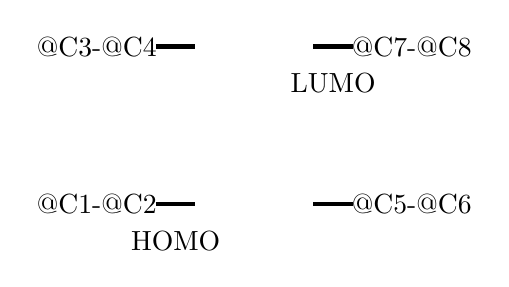
\begin{tikzpicture}
                \node at (0,2) {\chemfig{@{C3}-@{C4}}};
                \node          {\chemfig{@{C1}-@{C2}}};
                \draw [ultra thick]
                    (0.75,2) -- ++(0.5,0)
                    (0.75,0) -- node{\Large$\upharpoonleft\hspace{-1mm}\downharpoonright$} node[below=2mm]{HOMO} ++(0.5,0)
                ;
                
                \node at (4,2) {\chemfig{@{C7}-@{C8}}};
                \node at (4,0)  {\chemfig{@{C5}-@{C6}}};
                \draw [ultra thick]
                    (2.75,2) -- node[below=2mm]{LUMO} ++(0.5,0)
                    (2.75,0) -- node{\Large$\upharpoonleft\hspace{-1mm}\downharpoonright$} ++(0.5,0)
                ;
            \end{tikzpicture}
            \chemmove{
                \filldraw [thick,draw=orx,fill=ory] ($(C1)+(0.0018,0)$) to[bend right=120,looseness=600] ($(C1)+(-0.0018,0)$) -- cycle;
                \draw [thick,orx] ($(C1)+(0.0018,0)$) to[bend left=120,looseness=600] ($(C1)+(-0.0018,0)$) -- cycle;
                \filldraw [thick,draw=orx,fill=ory] ($(C2)+(0.0018,0)$) to[bend right=120,looseness=600] ($(C2)+(-0.0018,0)$) -- cycle;
                \draw [thick,orx] ($(C2)+(0.0018,0)$) to[bend left=120,looseness=600] ($(C2)+(-0.0018,0)$) -- cycle;
                \filldraw [thick,draw=orx,fill=ory] ($(C3)+(0.0018,0)$) to[bend right=120,looseness=600] ($(C3)+(-0.0018,0)$) -- cycle;
                \draw [thick,orx] ($(C3)+(0.0018,0)$) to[bend left=120,looseness=600] ($(C3)+(-0.0018,0)$) -- cycle;
                \draw [thick,orx] ($(C4)+(0.0018,0)$) to[bend right=120,looseness=600] ($(C4)+(-0.0018,0)$) -- cycle;
                \filldraw [thick,draw=orx,fill=ory] ($(C4)+(0.0018,0)$) to[bend left=120,looseness=600] ($(C4)+(-0.0018,0)$) -- cycle;
                % 
                \filldraw [thick,draw=orx,fill=ory] ($(C5)+(0.0018,0)$) to[bend right=120,looseness=600] ($(C5)+(-0.0018,0)$) -- cycle;
                \draw [thick,orx] ($(C5)+(0.0018,0)$) to[bend left=120,looseness=600] ($(C5)+(-0.0018,0)$) -- cycle;
                \filldraw [thick,draw=orx,fill=ory] ($(C6)+(0.0018,0)$) to[bend right=120,looseness=600] ($(C6)+(-0.0018,0)$) -- cycle;
                \draw [thick,orx] ($(C6)+(0.0018,0)$) to[bend left=120,looseness=600] ($(C6)+(-0.0018,0)$) -- cycle;
                \filldraw [thick,draw=orx,fill=ory] ($(C7)+(0.0018,0)$) to[bend right=120,looseness=600] ($(C7)+(-0.0018,0)$) -- cycle;
                \draw [thick,orx] ($(C7)+(0.0018,0)$) to[bend left=120,looseness=600] ($(C7)+(-0.0018,0)$) -- cycle;
                \draw [thick,orx] ($(C8)+(0.0018,0)$) to[bend right=120,looseness=600] ($(C8)+(-0.0018,0)$) -- cycle;
                \filldraw [thick,draw=orx,fill=ory] ($(C8)+(0.0018,0)$) to[bend left=120,looseness=600] ($(C8)+(-0.0018,0)$) -- cycle;
            }
            \caption{Thermal $[2+2]$ MOs.}
            \label{fig:22Orba}
        \end{subfigure}
        \begin{subfigure}[b]{0.45\linewidth}
            \centering
            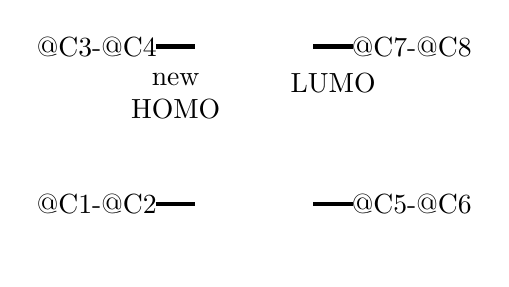
\begin{tikzpicture}
                \node at (0,2) {\chemfig{@{C3}-@{C4}}};
                \node          {\chemfig{@{C1}-@{C2}}};
                \draw [ultra thick]
                    (0.75,2) -- node{\Large$\downharpoonright$} node[below=2mm,align=center]{new\\HOMO} ++(0.5,0)
                    (0.75,0) -- node{\Large$\upharpoonleft$} node[below=2mm]{\phantom{HOMO}} ++(0.5,0)
                ;
                
                \node at (4,2) {\chemfig{@{C7}-@{C8}}};
                \node at (4,0)  {\chemfig{@{C5}-@{C6}}};
                \draw [ultra thick]
                    (2.75,2) -- node[below=2mm]{LUMO} ++(0.5,0)
                    (2.75,0) -- node{\Large$\upharpoonleft\hspace{-1mm}\downharpoonright$} ++(0.5,0)
                ;
            \end{tikzpicture}
            \chemmove{
                \filldraw [thick,draw=orx,fill=ory] ($(C1)+(0.0018,0)$) to[bend right=120,looseness=600] ($(C1)+(-0.0018,0)$) -- cycle;
                \draw [thick,orx] ($(C1)+(0.0018,0)$) to[bend left=120,looseness=600] ($(C1)+(-0.0018,0)$) -- cycle;
                \filldraw [thick,draw=orx,fill=ory] ($(C2)+(0.0018,0)$) to[bend right=120,looseness=600] ($(C2)+(-0.0018,0)$) -- cycle;
                \draw [thick,orx] ($(C2)+(0.0018,0)$) to[bend left=120,looseness=600] ($(C2)+(-0.0018,0)$) -- cycle;
                \filldraw [thick,draw=orx,fill=ory] ($(C3)+(0.0018,0)$) to[bend right=120,looseness=600] ($(C3)+(-0.0018,0)$) -- cycle;
                \draw [thick,orx] ($(C3)+(0.0018,0)$) to[bend left=120,looseness=600] ($(C3)+(-0.0018,0)$) -- cycle;
                \draw [thick,orx] ($(C4)+(0.0018,0)$) to[bend right=120,looseness=600] ($(C4)+(-0.0018,0)$) -- cycle;
                \filldraw [thick,draw=orx,fill=ory] ($(C4)+(0.0018,0)$) to[bend left=120,looseness=600] ($(C4)+(-0.0018,0)$) -- cycle;
                % 
                \filldraw [thick,draw=orx,fill=ory] ($(C5)+(0.0018,0)$) to[bend right=120,looseness=600] ($(C5)+(-0.0018,0)$) -- cycle;
                \draw [thick,orx] ($(C5)+(0.0018,0)$) to[bend left=120,looseness=600] ($(C5)+(-0.0018,0)$) -- cycle;
                \filldraw [thick,draw=orx,fill=ory] ($(C6)+(0.0018,0)$) to[bend right=120,looseness=600] ($(C6)+(-0.0018,0)$) -- cycle;
                \draw [thick,orx] ($(C6)+(0.0018,0)$) to[bend left=120,looseness=600] ($(C6)+(-0.0018,0)$) -- cycle;
                \filldraw [thick,draw=orx,fill=ory] ($(C7)+(0.0018,0)$) to[bend right=120,looseness=600] ($(C7)+(-0.0018,0)$) -- cycle;
                \draw [thick,orx] ($(C7)+(0.0018,0)$) to[bend left=120,looseness=600] ($(C7)+(-0.0018,0)$) -- cycle;
                \draw [thick,orx] ($(C8)+(0.0018,0)$) to[bend right=120,looseness=600] ($(C8)+(-0.0018,0)$) -- cycle;
                \filldraw [thick,draw=orx,fill=ory] ($(C8)+(0.0018,0)$) to[bend left=120,looseness=600] ($(C8)+(-0.0018,0)$) -- cycle;
            }
            \caption{Photochemical $[2+2]$ MOs.}
            \label{fig:22Orbb}
        \end{subfigure}\\[4em]
        \begin{subfigure}[b]{0.45\linewidth}
            \centering
            \chemfig{@{C3}-[,0.5](-[6,2.5,,,opacity=0](-[4,0.5]@{C1})(-[,0.5]@{C2}))-[,0.5]@{C4}}
            \chemmove{
                \filldraw [thick,draw=orx,fill=ory] ($(C1)+(0.0018,0)$) to[bend right=120,looseness=600] ($(C1)+(-0.0018,0)$) -- cycle;
                \draw [thick,orx] ($(C1)+(0.0018,0)$) to[bend left=120,looseness=600] ($(C1)+(-0.0018,0)$) -- cycle;
                \filldraw [thick,draw=orx,fill=ory] ($(C2)+(0.0018,0)$) to[bend right=120,looseness=600] ($(C2)+(-0.0018,0)$) -- cycle;
                \draw [thick,orx] ($(C2)+(0.0018,0)$) to[bend left=120,looseness=600] ($(C2)+(-0.0018,0)$) -- cycle;
                \filldraw [thick,draw=orx,fill=ory] ($(C3)+(0.0018,0)$) to[bend right=120,looseness=600] ($(C3)+(-0.0018,0)$) -- cycle;
                \draw [thick,orx] ($(C3)+(0.0018,0)$) to[bend left=120,looseness=600] ($(C3)+(-0.0018,0)$) -- cycle;
                \draw [thick,orx] ($(C4)+(0.0018,0)$) to[bend right=120,looseness=600] ($(C4)+(-0.0018,0)$) -- cycle;
                \filldraw [thick,draw=orx,fill=ory] ($(C4)+(0.0018,0)$) to[bend left=120,looseness=600] ($(C4)+(-0.0018,0)$) -- cycle;
                % 
                \node [right=2mm] at (C4) {LUMO};
                \node [right=2mm] at (C2) {HOMO};
                % 
                \draw [rex,thick,-] ([xshift=-1.5mm,yshift=-5mm]C3.center) to[bend right=20] node[left]{X} ([xshift=-1.5mm,yshift=5mm]C1.center);
                \draw [cyan,thick,-] ([xshift=1.5mm,yshift=-5mm]C4.center) to[bend left=20] node[right]{$\checkmark$} ([xshift=1.5mm,yshift=5mm]C2.center);
            }
            \vspace{2em}
            \caption{Thermal orbitals in 3D space.}
            \label{fig:22Orbc}
        \end{subfigure}
        \begin{subfigure}[b]{0.45\linewidth}
            \centering
            \chemfig{@{C3}-[,0.5](-[6,2.5,,,opacity=0](-[4,0.5]@{C1})(-[,0.5]@{C2}))-[,0.5]@{C4}}
            \chemmove{
                \draw [thick,orx] ($(C1)+(0.0018,0)$) to[bend right=120,looseness=600] ($(C1)+(-0.0018,0)$) -- cycle;
                \filldraw [thick,draw=orx,fill=ory] ($(C1)+(0.0018,0)$) to[bend left=120,looseness=600] ($(C1)+(-0.0018,0)$) -- cycle;
                \filldraw [thick,draw=orx,fill=ory] ($(C2)+(0.0018,0)$) to[bend right=120,looseness=600] ($(C2)+(-0.0018,0)$) -- cycle;
                \draw [thick,orx] ($(C2)+(0.0018,0)$) to[bend left=120,looseness=600] ($(C2)+(-0.0018,0)$) -- cycle;
                \filldraw [thick,draw=orx,fill=ory] ($(C3)+(0.0018,0)$) to[bend right=120,looseness=600] ($(C3)+(-0.0018,0)$) -- cycle;
                \draw [thick,orx] ($(C3)+(0.0018,0)$) to[bend left=120,looseness=600] ($(C3)+(-0.0018,0)$) -- cycle;
                \draw [thick,orx] ($(C4)+(0.0018,0)$) to[bend right=120,looseness=600] ($(C4)+(-0.0018,0)$) -- cycle;
                \filldraw [thick,draw=orx,fill=ory] ($(C4)+(0.0018,0)$) to[bend left=120,looseness=600] ($(C4)+(-0.0018,0)$) -- cycle;
                % 
                \node [right=2mm] at (C4) {LUMO};
                \node [right=2mm] at (C2) {new HOMO};
                % 
                \draw [cyan,thick,-] ([xshift=-1.5mm,yshift=-5mm]C3.center) to[bend right=20] node[left]{$\checkmark$} ([xshift=-1.5mm,yshift=5mm]C1.center);
                \draw [cyan,thick,-] ([xshift=1.5mm,yshift=-5mm]C4.center) to[bend left=20] node[right]{$\checkmark$} ([xshift=1.5mm,yshift=5mm]C2.center);
            }
            \vspace{2em}
            \caption{Photochemical orbitals in 3D space.}
            \label{fig:22Orbd}
        \end{subfigure}
        \caption{$[2+2]$ cycloaddition orbitals.}
        \label{fig:22Orb}
    \end{figure}
    \begin{itemize}
        \item Let's consider a $[2+2]$ cycloaddition between ethylene and itself.
        \item Since the reactants are identical, we may choose (arbitrarily and without loss of generality) which molecule reacts with its HOMO. It will then follow that the other molecule reacts with its LUMO.
        \begin{itemize}
            \item Thus, let the left (Figures \ref{fig:22Orba}-\ref{fig:22Orbb}) and bottom (Figures \ref{fig:22Orbc}-\ref{fig:22Orbd}) molecules react with their HOMO, and let the right/top molecules react with their LUMO.
        \end{itemize}
        \item In the thermal case, the HOMO and LUMO don't overlap well (Figure \ref{fig:22Orbc}).
        \begin{itemize}
            \item The phasings match on one side, but not on the other.
        \end{itemize}
        \item However, in a \emph{photochemical} reaction, we excite an electron up one energy level (Figure \ref{fig:22Orbb}).
        \begin{itemize}
            \item Recall that we briefly discussed this phenomenon in Figure \ref{fig:thermPhot}.
            \item This excitation gives us a new HOMO.
        \end{itemize}
        \item The new HOMO can react with the LUMO (same as thermal) because the phasing now matches!
    \end{itemize}
    \item In Figure \ref{fig:22Orb}, we could choose the HOMO and LUMO arbitrarily because the reactants were identical.
    \begin{itemize}
        \item But in Figure \ref{fig:22Cyclo}, the reactants are \emph{not} identical.
        \item Moreover, it turns out that there \emph{is} a preference for which of these two species absorbs the photon!
    \end{itemize}
    \pagebreak
    \item The species that can form the more stable diradical will absorb the light.
    \begin{figure}[h!]
        \centering
        \footnotesize
        \schemestart
            \chemfig{*6(@{C2}----(=O)-@{C1}=[@{1}])}
            \arrow{->[$h\nu$]}
            \chemleft{[}\subscheme{
                \chemfig{*6(\charge{180=\.}{}----(=O)-\charge{180=\.}{}(-[4,0.2,,,opacity=0])-)}
                \arrow{<->}
                \chemfig{*6(\charge{180=\.}{}----(-\charge{0=\.}{O})=-)}
            }\chemright{]}
        \schemestop
        \chemmove{
            \draw [curved arrow={2pt}{2pt},-{Stealth[round,scale=1.1,inset'=0pt 0.55,harpoon]}] (1) to[bend left=85,looseness=3] (C1);
            \draw [curved arrow={2pt}{2pt},-{Stealth[round,scale=1.1,inset'=0pt 0.55,harpoon,swap]}] (1) to[bend right=85,looseness=3] (C2);
        }
        \caption{Systems with more stable excited states preferentially absorb light.}
        \label{fig:photoStable}
    \end{figure}
    \begin{itemize}
        \item In the context of Figure \ref{fig:22Cyclo}, the enone will absorb the photon because its diradical is resonance-stabilized.
        \item Thus, the enone will react with its (new) HOMO.
        \begin{itemize}
            \item Note that this new HOMO is also a SOMO!
            \item Per Figure \ref{fig:22Orbb}, the photoexcited species will actually have \emph{two} SOMOs.
        \end{itemize}
        \item For more context, check out \textcite{bib:Clayden}: The textbook actually does an excellent job covering this photochemistry stuff!!
    \end{itemize}
    \item Looking ahead (Friday).
    \begin{itemize}
        \item We will begin with a bit more content on cycloadditions that we could not get to today.
        \item After that, we will cover electrocyclizations.
        \item It's going to be a long lecture, but you'll have the weekend to digest it.
    \end{itemize}
\end{itemize}




\end{document}